% !TEX root = ../0-main-LN.tex

\setcounter{theExample}{1}
\setcounter{chapter}{0}

\chapter{函数与极限}

函数与极限是微积分理论中最基础和最核心的概念,也是定义
微分和积分的基础。熟练掌握常用函数的特性,理解极限的概念与性质,
并会在一定程度上加以应用,是真正理解微积分的第一步。

极限的定义(更具体地称为“$\e-\delta$”或“$\e-N$”定义)可能是大多数人
在微积分学习中遇到的第一个难点(因人而异),因为它兼具形式的抽象性和
逻辑的复杂性(必须严谨、准确)。学会用数学和逻辑的语言表达某个概念、某个
命题,并能将推理、分析的过程严谨、准确地叙述出来,也是通过微积分的学习
需要锻炼和培养的能力。

\section{集合、映射与函数}

\subsection{集合}

我们目前使用的集合概念,一般被认为来源于数学家Cantor的定义(1974),
他的表述是:所谓{\it 集合},是指把一些个体({\it 元素}) 
放在一起考虑时所形成的整体。
\ps{对于集合,“我们只需描述它,而不必给出精确的定义”}

我们可能用到的相关的符号可分为两类:
\begin{itemize}
  \item 关系符号:$\subset, \in, =, \subseteq, \neq$
  \item 运算符号:$\cap,\cup, \setminus, \bar{A}, \times, +, - $\quad ({\it
  依次为:交、并、差、补、笛卡尔积、不交并、差})
\end{itemize}
	
本门课程中常见(用)的集合有:
$$\mathbb{N}\subset\mathbb{Z}\subset\mathbb{Q}
\subset\mathbb{R}\subset\mathbb{C}$$
从左到右依次为:{\kaishu 自然数集}
\ps{\vspace{-1cm}国内教材一般约定,自然数集包含数$0$}、
{\kaishu 整数集}\ps{Z是德语Zahlen(数)的首字母}、{\kaishu 有理数集}
、{\kaishu 无理数集}和{\kaishu 复数集}。

通过集合的{\it 笛卡尔积}“$\times$” 可以定义更{\it“高维”}的集合,
例如:$\mathbb{R}$表示数轴(上的所有点构成的集合),则
$$\mathbb{R}^2=\mathbb{R}\times\mathbb{R}$$
表示全平面(上的所有点构成的集合)。

\subsubsection*{区间和邻域}

讨论函数的定义域和值域是,我们常常会用到区间和领域这两个概念。

具体来说,给定$a,b\in\mathbb{R},a<b$,可定义一个开区间
$$(a,b)=\{x\in\mathbb{R}|a<x<b\}.$$

一般来说,我们记实数集
$$\mathbb{R}=(-\infty,+\infty)$$

{\baa 注意:由于$\pm\infty$都不是具体的数,因此在本门课程中,
除非特别说明,形如
$$x=+\infty\quad\mbox{或}\quad x=-\infty$$
的写法总是错误的,而只能写
$$x\to+\infty\quad\mbox{或}\quad x\to\infty.$$
}

{\bf 邻域}是区间的另一中表示方法,它的一般形式为
$$U(x_0,\delta),$$
其中$x_0$表示邻域的中心,$\delta$为领域的半径,如非特别说明,
领域一般为开区间。例如:
$$U(a,\delta)=(a-\delta,a+\delta)=\{x\in\mathbb{R}||x-a|<\delta\}.$$
$U(x_0,\delta)$的直接解释是:实数中所有与$x_0$的距离(差的绝对值)
小于$\delta$的数(点)构成的集合。

\bs

{\bf 课堂练习:}$(a,b)=\underline{\hspace{4cm}}$
\ifhint\ps{$U\left(\df{a+b}2,\df{b-a}2\right)$}\fi

\bs

有时候,我需要考虑不包含中心的领域,也即{\kaishu 去心领域},记为
$$
U_0(a,\delta)\quad\mbox{或}\quad U^0(a,\delta)$$
对应的区间为$(a-\delta,a+\delta)-\{a\}$
(或$\{x\in\mathbb{R}|0<|x-a|<\delta\}$)。

有时候,我们也会用到所谓的{\kaishu 无穷邻域},其定义为
$$\{x\in\mathbb{R}||x-x_0|>M\},\;M>0,$$
表示与点$x_0$的距离超过$M$的所有点构成的集合。我们可以将无穷领域想象
成以{\kaishu 无穷远点}\ps{\baa 因为无穷远点不是一个数,为了避免误解,我们不会将无穷邻域
写成类似 $U(\infty ,M)$的形式}
(现实中是不存在的)为中心的领域。

最后,还有所谓的{\kaishu 左(右)半邻域},例如:点$a$的右半邻域为
$$\{x\in\mathbb{R}|a<x<a+\delta\}.$$

\bs
\centerline{注:灰色底色部分的内容为扩展知识,了解即可,不要求掌握}
\begin{shaded}
	{\bf 集合论、Russell Paradox与公理系统}

	Cantor在1874年提出的集合概念及其相关的理论——统称{\kaishu 集合论},通常被也称为{\kaishu 朴素集合论}。集合论的提出为整个数学的研究
	奠定了重要基础,使得众多的数学理论得以变得更加严谨和系统。对于这一
	成就,历史上有过一些重要的评述,其中被广泛传播的是Poincaré在1900的
	国际数学家大会所说:{\kaishu
	 “\ldots 借助集合论概念,
	 我们可以建造整个数学大厦\ldots  
	 今天,我们可以说绝对的严格性已经达到了\ldots”}。
	
	然而,现实其实并不那么乐观,1901年,英国数学家——也有人说是哲学家
	——Russell提出了他著名的悖论

	\pss{\centering
	\includegraphics[width=0.7\marginparwidth]{./images/ch01/Russell.jpg}\\
	\href{https://en.wikipedia.org/wiki/Bertrand_Russell}{B. Russell(1872-1970)}
	}

	\centerline{\kaishu 只给不给自己理发的人理发的理发师该不该给自己理发?}
	
	转换成集合论的语言,可以表述为:

	\centerline{\kaishu 由所有不包含集合自身的集合所构成
	的集合是不是一个集合?}

	其中的矛盾是非常明显的。设$A$为上述集合,则
	$$A=\{x|x\notin x\}.$$ 
	如果$A\in A$,则根据以上定义,$A\notin A$;反之,如果$A\notin A$,
	则必有$A\in A$。

	那么到底是$A\in A$还是$A\notin A$呢? 一个简单的命题居然导出了
	自相矛盾的结论,这从根本上动摇了数学大厦的根基。Cantor的集合定义的
	本质是一个命题总会对应某个集合,这看来是错误的!

	Russell Paradox({\kaishu 罗素悖论})的出现引发了著名的
	{\kaishu 第三次“数学危机”}。数学家Frege于1901年完成《算术基础》
	时,说了这样一段话:{\kaishu 在工作结束之后发现那大厦的基础已经动摇,
	对于一个科学工作者来说,没有比这更不幸的了。}
	
	Cantor的集合定义也被称为{\kaishu 无限抽象原则},为了避免类似
	悖论的出现,数学家们对其提出了若干修正的方案,这些方案虽然各不相同,
	当共同的一点就是采用{\kaishu 有限抽象原则}替代了无限抽象原则。
	有限抽象原则的描述如下:如果已知一个集合和一个给定的条件,则该
	集合中所有满足条件的元素{\it 可以}构成一个集合。显然,在这样的
	原则之下,是无法定义所谓的包含有所集合的集合或包含所有不包含自己的
	集合的集合的。

	新的集合论被统称为{\kaishu 公理化集合论},不同于朴素集合论的直观,
	公理化集合论更强调理论自身的严谨自洽(不能自相矛盾)。最著名的公理化
	集合论是所谓的{\kaishu ZF(Zermelo-Fraenkel)公理化集合论}
	(\href{https://en.wikipedia.org/wiki/Zermelo–Fraenkel_set_theory}
	{Wikipedia: Zermelo-Fraenkel Set Theory}),
	其中通过引入{\kaishu 替代公理}避免了矛盾的产生。
	  
	{\bf 命题:}在ZF/ZFC中,无法定义包含所有集合的集合。
	
	证:反证法。设$A$是一个这样的集合。定义
	$$B=\{x\in A|x\notin x\}.$$
	若$B\in A$,则必有$B\in B$或$B\notin B$。
	而若$B\in B$,可推出$B\notin B$;同理,
	由$B\notin B$,也可推出$B\in B$。
	从而$B\notin A$,推出矛盾,故知假设错误,也即$A$是不存在。\fin

	公理(Axiom)就是无须证明即为正确的命题。关于其定义有如下的描述:
	\begin{itemize}
	  \item Engles:数学上的所谓公理,是数学需要用
	  作自己出发点的少数思想上的规定 
	  \item ZFS系统:公理就是一些关于逻辑符号{“$\in$”}和{字母}的组合使用方法的约定
	  \item {\kaishu 公理化方法}是构建现代数学理论体系的基石。
	\end{itemize}

	看了上面的故事,我们不禁要问一个问题:{\bf 数学等于绝对的真理吗?}
	答案看来并不是那么肯定,比较严谨的表述应该是,{\kaishu 
	数学在特定的假定之下,按照特定的逻辑推理方法,
	所得出的结论可以被认为是正确的}。

	那么,又出现了另一个问题:{\bf 我们是不是不应该相信数学呢?}
	答案是肯定的,在绝大多数情况下,数学的结论都和我们的直觉高度一致,
	也正因为如此,数学才被认为是最有用和最基础的科学理论。
	就我们目前所知,类似于前面的悖论,只在极少数特定的情况下
	存在,并不影响我们将数学理论与直觉相统一,方便我们从直觉与观察中
	抽象和发现数学,同时将数学应用于实际的问题中。
	
	注:ZFC事实上包含了无穷多个公理,因为它所使用的替代公理实际上
	是公理模式。已知ZFC和ZF集合论二者都是不能用有限数目个公理来完全公理化的。
	
	\bs

	{\bf 讨论:}公理(Axiom)、定理(Theorem)、定律(Law)、假设(Assumption)、
	引理(Lemma)、推论(Corallary)、猜想(Conjuction)有何异同?
	
	答:这些概念都是对自然规律或数学规则的表达。
	
	公理是数学及其相近领域所使用的概念,即在数学理论体系中无须证明即
	视为正确的命题(例如:两点之间直线最短),是数学理论体系的出发点。
	通过推理和演绎,我们可以在公理的基础上进一步推出新的结论,
	这些结论我们通常称为定理,引理和推论则是定理推导的中间和后续结果。
	使用不同的公理作为出发点,可能得到完全不同的理论体系,
	例如:非欧几何的多条基本公设(公理的另一种说法)就是和欧式几何不同的,
	这导致二者的理论体系看起来大相径庭。
	
	我们目前所使用的公理多数来源于生活中的直观体验,是一种对直觉
	观察的抽象描述。而由于	我们对自然世界认识的局限性,这些描述
	本身可能是不精确甚至是不正确的。从这个意义上说,我们
	更应该说公理其实是我们对于客观规律的假定,是先验的,
	但也是可以有所调整和变化的。
	
	定律也具有类似的特点,因为人类总是在不断改进和加深对于自然世界
	的认识。定律更多地出现于物理、化学等非抽象领域,
	体现的是对自然规律的描述。定律背后通常存在一些的
	基本假定(例如:原子是不可分的、光既是例子又是波),
	定律的发现需要以重复实验为基础,定律的描述中一部分是可以用
	数学工具来刻画的(例如万有引力定律、质能方程)。
	
	公理、定理、定律的共性之处在于它们在各自的领域中或背景下,
	都被视为是“正确的”(请注意在数学中正确和可证明有时是被混同的),
	是被验证、证明或直接假定为真的命题,而猜想则是被
	猜测为真,但未经过这些过程,所以仍无法断言为真的。
	当今的数学界,仍有大量的猜想有待证明或证否,
	这些问题所代表的恰恰是数学的最前沿。\fin 
\end{shaded}
	
\subsubsection{实数集的性质}

实数集$\mathbb{R}$具有两个基本的性质:
\begin{enumerate} 
	\setlength{\itemindent}{1cm}
  \item {\it 有序性:}即任何两个实数均可以比大小;
  \hfill (注:$\mathbb{R}^2$、$\mathbb{C}$不具备有序性) 
  \item {\it 完备性(连续性): }实数集与数轴上的点之间存在一一对应。
\end{enumerate}

完备性的等价\ps{等价关系的证明参见菲赫金哥尔茨的《微积分学教程》绪论第2节}
命题是所谓的{\it 确界原理}
\begin{thx}
	{\bf 确界原理(连续性公理):}非空有上(下)界的实数集
	必有实数的{\it 上(下)确界} ,且该上(下)确界为实数。
\end{thx}
为了更好地理解确界原理,必须对集合的有界性以及上(下)界和
上(下)确界的概念有非常准确的理解:
\begin{thx}
	{\bf 上界:}$M\in\mathbb{R}$称为集合$A\subset\mathbb{R}$的上界,是指:对任意$x\in A$,均有$x\leq M$。
	
	{\bf 集合$A$有上界:}存在$M\in\mathbb{R}$为$A$的上界
	(显然上界是不唯一的!)
	
	{\bf 集合$A$有界:}即$A$既有上界也有下界。
\end{thx}	
设$M$和$m$分别为$A$的上界和下界,令$M^*=\max\{|m|,|M|\}$,则可以证明,对
任意$x\in A$,有$-M^*\leq x\leq M^*$,或$|x|\leq M^*$。这个命题
也常常作为集合有界的定义。
\begin{thx}
	{\bf 上确界:}
	$M_0\in\mathbb{R}$称为集合$A\subset\mathbb{R}$的上确界
	(记为$M_0=\mathrm{sup}A$,下确界记为:$\mathrm{inf}A$),
	是指:$M_0$是$A$的最小上界,或者说应同时满足:
	\begin{enumerate}[(1)]
	  \item $M_0$是$A$的上界,即:对任意$x\in A$,均有$x\leq M_0$;
	  \item $A$的任意上界都不小于$M_0$,即:若$M$为$A$的一个上界,
	  则$M_0\leq M$。
	\end{enumerate}
\end{thx}

\pss{缩写符号:\\ $\Leftrightarrow$:等价\\ $\forall$:任意
\\ $\exists$:存在}

{\bf $M_0$为$A$的上确界}的另一个{\it 数学定义}:
{\it 对任意(小)的$\e>0$,
都(至少)存在一个$x_{\e}\in A$,使得$M_0-\e<x_{\e}\leq M_0$,}
或者简写为:
$$M_0=\mathrm{sup}A\;\Leftrightarrow\;
\forall\e>0,\;\exists x_{\e}\in A,\;M_0-\e<x_{\e}\leq M_0.$$

\bs

{\bf 思考:}上面这个对上确界的数学定义,与前面我们讨论
的上确界的概念之间是什么关系?你能否证明它们是等价的?

\pss{大多数时候,我们并不严格区分数学定义和概念,只是数学定义通常
会用更抽象的数学符号和更严谨的逻辑语言来表达,今后我们所说的定义即指
数学定义或概念}

\ifhint
答:是等价的。证明如下:

首先,设$M_0$是集合$A$的最小上界,证明对任意$\e>0$,
存在$x_{\e}\in A$,使得$x_{\e}\in(M_0-\e,M_0)$。
反证法。若对某个$\e_0>0$,不存在这样的$x_{\e_0}$,则
意味着对任意的$x\in A$,均不满足$x\in(M_0-\e_0,M_0)$。
由此可知,任意$x\in A$,均满足$x\leq M_0-\e_0$,
这说明$M_0-\e_0$也是$A$的一个上界,而$M_0-\e_0<M_0$,
这就与$M_0$是$A$的最小上界的条件相矛盾了,从而可知
假设错误,即证。

另一方面,设对任意$\e>0$,都存在$x_{\e}\in A$,
使得$x_{\e}\in(M_0-\e,M_0)$,证明$M_0$是$A$最小的上界。
反证法,若$M_0$不是$A$的最小上界,则必有某个$M_1<M_0$
也是$A$的上界,即对任意$x\in A$,总有$x\leq M_1$。
令$\e_1=\frac12(M_0-M_1)$,则对任意$x\in A$,
均有$x\notin(M_0-\e_1,M_0)$,从而与已知矛盾,故假设错误,即证。
\fin
\fi

\bs

{\bf 思考:}上确界和最大值有什么异同?如何确定一个集合的上确界?

\ifhint
答:若该集合中存在最大值,则最大值就是其上确界。如果该集合中没有最大值,
则其取其上界构成的集合的最小值。
\fi

\bs

{\bf 讨论:}有理数集是否满足连续性公理?

\ifhint
答:不满足!准确地说就是:有理数集的非空有上界的子集,
其上确界未必是有理数(虽然肯定是实数)!为了说明这一点,来看下面的例子:

考虑集合$A=\left\{\left(1+\frac 1n\right)^n
|n\in\mathbb{N}\right\}$,因为
有理数的有限次四则运算仍是有理数,故显然$A\subset\mathbb{Q}$。
如下图所示,集合$A$中的点如果按照
$n$从小到大的顺序排列,恰好是构成一个随$n$单调递增有上界($3$就是它的一个上界)的数列,也即:
$$\left(1+\frac11\right)^1<\left(1+\frac12\right)^2<\left(1+\frac13\right)^3<\ldots
\left(1+\frac1n\right)^n<\ldots<3.$$
\begin{figure}[h]
	\centering
	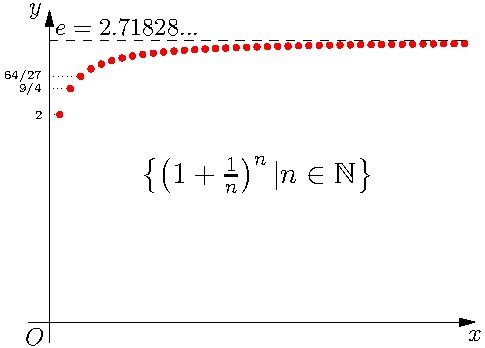
\includegraphics[width=0.5\textwidth]{./images/ch01/e-notin-N.pdf}
	\caption{有理数列$\left\{\left(1+\df1n\right)^n\right\}$构成的集合
	上确界为$e\notin\mathbb{Q}$}
	\label{fig:2.1}
\end{figure}
根据常用极限\ps{$e=\lim\limits_{n\to\infty}\left(1+\df1n\right)^n$}
不难看出$e=\mathrm{sup}A$,但$e\notin\mathbb{Q}$,
故有理数集不满足连续性公理。\fin

又比如这样一个例子:$A=\{x\in\mathbb{Q}|x\geq 0,\;x^2<2\}$,显然,
$\mathrm{sup}A=\sqrt2\notin\mathbb{Q}$。
\fi

\bs
{\bf 思考:}任给一个实数,如何构造一个有理数集合,使得该实数恰好为
该有理数集合的上(下)确界?

\ifhint
答:方法很多,以下给出其中一种。

设该实数为:
$$a=A.a_1a_2a_3\ldots a_n\ldots,$$
其中$A$为整数,$a_i(i=1,2,\ldots)$均为$0,1,\ldots,9$之中的
个位数。

定义如下的两个集合:
$$A_1=\left\{A.a_1a_2\ldots a_n-\frac1n
\Big|n\in\mathbb{Z}^+\right\},
\quad
A_2=\left\{A.A.a_1a_2\ldots a_n-\frac{\sqrt2}n\Big|
n\in\mathbb{Z}^+\right\},$$
因为有理数与有理数的和仍为有理数,而有理数与无理数的和必为无理数,
故易知$A_1\subset\mathbb{Q}$,$A_2\subset\mathbb{R}-\mathbb{Q}$。
此外,容易验证
$$\sup A_1=\sup A_2=a.$$
\fin
\fi

\begin{shaded}
	{\bf 开集与闭集}
	
	集合$A\subset\mathbb{R}$为{\bf 开集},是指:对任意$x\in A$,
	均存在$\delta>0$,使得
	$U(x,\delta)\subset A.$
	
	集合$A\subset\mathbb{R}$为{\bf 闭集},是指其补集
	$\bar{A}=\mathbb{R}-A$为开集。
	
	例如:所有的开区间都是开集,所有的闭区间为闭集;
	我们通常{\it 约定空集$\phi$既是开集又是闭集},
	因此{\it 实数集$\mathbb{R}$既是开集又是闭集}。
	
	点$a$称为集合$A$的{\bf 内点},是指:存在$\delta>0$,
	使得$U(a,\delta)\subset A$。显然开集中的点均为其内点!
	
	点$a$称为集合$A$的{\bf 外点},是指:存在$\delta>0$,
	使得$U(a,\delta)\cap A=\phi$,
	或者说$a$为$A$的补给的内点。
	
	点$a$称为集合$A$的{\bf 边界点},是指$a$既不是$A$的内点,
	也不是$A$的外点,或者说
	对任意的$\delta>0$,$U(a,\delta)\cap A\ne\phi$。
	
	显然,闭集可以视为其最大开子集和其所有边界点的并。
	
	\egz 指出以下集合哪些是开集,哪些是闭集?
	\begin{enumerate}[(1)]
	  \setlength{\itemindent}{1cm}
	  \item $\{1,2,3,5\}$\hfill({\it 闭})
	  \item $U_0(1,3)$\hfill({\it 开})
	  \item 自然数集\hfill({\it 闭})
	  \item 有理数集\hfill({\it 既非开又非闭})
	  \item 无理数集\hfill({\it 既非开又非闭})
	  \item $\left\{\left(1+\frac
	  1n\right)^n|n\in\mathbb{N}\right\}+\{e\}$\hfill({\it 闭})
	\end{enumerate}
\end{shaded}

\subsection{映射}

映射通常被定义为,事物之间“一对一”或“多对一”的依赖关系。更形象地说,可以将
映射视为一种输入输出过程,“一对一”或“多对一”保证了
一个输入只能得到一个特定的输出,因此结果是{\it 无歧义}
\ps{无歧义是保证数学论证简明性的一个常见的要求}
的。从这个意义上说,对于映射的这种定义方式也是一种{\it 约定}。
由集合$A$到$B$的映射$f$一般记为:
$$f:A\mapsto B \quad\mbox{或}\quad y=f(x),\;x\in A,y\in B$$

{\it 映射的三要素:}定义域、值域、对应关系,任何一项不明确都不足以确定一个函数,或者说,
两个映射在这三方面有一点不同,则应视为不同的映射。
\ps{之所以有时候只关心定义域和对应关系,前提是默认假设映射为满射}

{\bf 函数}通常是指数集之间的映射。有时也推广到高维的数集,例如
$$z=x^2+y^2,\;(x,y)\in\mathbb{R}^2.$$

\egz 假设下列函数均取{\it 自然定义域}
\ps{即在$\mathbb{R}$中可取到的最大定义范围},
且均为满射,指出其中哪些是完全相同的?
$$x,\quad |x|,\quad e^{\ln x},\quad \ln(e^x),\quad \sqrt{x^2},\quad
\frac{x^2-4}{x-2}-2,$$
$$\sin(\arcsin x),\quad \arcsin(\sin x), \quad \tan(\arctan x)$$

与映射和函数相关的概念还有{\bf 单射、满射、一一映射(双射)},不再一一赘述。

\begin{shaded}
	\pss{\centering
	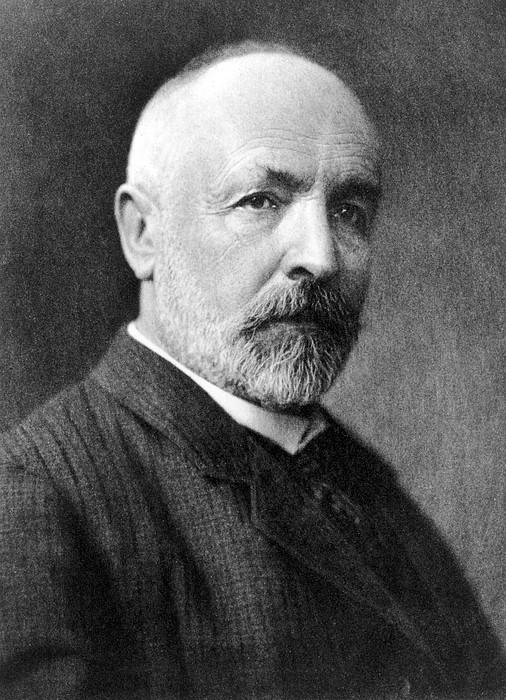
\includegraphics[width=0.7\marginparwidth]{./images/ch01/Cantor.jpg}\\
	\href{https://en.wikipedia.org/wiki/Georg_Cantor}{G. Cantor(1845-1918)}
	}
	{\bf 一一映射与无穷集合}

	考虑一个问题:如何比较两个集合中元素的个数?

	一般来说,我们称两个元素个数相同的集合为{\it 等势}的。对于
	元素有限的集合来说,判断两个集合是否等势也很容易的。困难在于
	如何判定两个元素个数不是有限的集合等势!

	Cantor的一大贡献就是给出了这个问题目前最广为接受的方法,或者说,
	他实际上给出了集合等势的严格定义:
	如果存在集合$A$和$B$之间的一一映射,则$A$和$B$是{\bf 等势}的。
	紧接着,他证明了一系列重要的集合之间的等势关系。
	
	\bs

	\egz 以下集合两两等势吗,为什么?
	({\baa 正确的命题须给出证明,错误的则只需举出反例})
	\begin{enumerate}[(1)]
	  \setlength{\itemindent}{1cm}
	  \item 自然数与正偶数({$\surd$})
	  \item 自然数与整数({$\surd$})
	  \item 自然数与有理数({$\surd$})
	  \item 区间$(0,1)$中的实数与$\mathbb{R}$中({$\surd$},例如:$y=\df1{e^x+1}$)
	  \item 自然数与实数({$\times$})
	\end{enumerate}
	
	\bs
	提示:一个集合与自然数集等势,等价于这个集合中的所有数可以不重复地
	排成一列,形象地说,就是可以把这个集合中所有的数一个个地数完而没有任何重复
	与遗漏。

	例如要证明整数集与自然数集等势,显然只需这样来排列整数集:
	$$0,1,-1,2,-2,3,-3,4,-4,\ldots,$$
	很容易看出这样的排列是既没有遗漏也没有重复的,
	事实上等于给出了从自然数集到整数集的一一映射。
	显然要证明自然数集和正偶数集等势也是一样的容易。
	
	\bs
	(3)\;参照上面的作法,要证明自然数集与有理数集等势,
	也只需要考虑能否找到一种方式
	将所有的有理数排成一列,既不重复也不遗漏。
	参考图\ref{fig:1-2},我们可以先说明所有的正有理数
	可以排成一列:
	$$1,2,\df12,3,\df13,4,\df32,\df23,\df14,5,\df15,6,\df52,
	\df43,\df34,\df25,\df16,\ldots,$$
	从图上不难看出,这个排列事实上给出了从自然数集到正有理数集的一一映射。
	接下来,在其中逐个插入对应的负有理数,即可得到从自然数集到有理数集的
	一一映射。
	
	{\bf 思考:}能否证明$\mbb{Z}$和$\mbb{Z}^2$是等势的?任意给定某个$n$,
	$\mbb{Z}$和$\mbb{Z}^n$也等势吗?$\mbb{Q}$和$\mbb{Q}^n$呢?
	$\mbb{R}$和$\mbb{R}^n$呢?
	
	(5)\;我们只需证明不存在自然数集到区间$(0,1)$的一一
	映射即可。
	
	反证法(据说这是Cantor最初的证明方法):假设存在自然数集到$(0,1)$的
	一一映射,这意味着$(0,1)$中所有的数可以排成一个数列,没有重复也没有遗漏,
	设其中第$i$个数表示为
	$$a_i=a_{i1}a_{i2}a_{i3}a_{i4}\ldots,$$
	其中$a_{ij}(j=1,2,\ldots)$都是$0$到$9$之间的个位整数。
	
	接下来,我们构造一个新的数
	$$a_*=a_{*1}a_{*2}a_{*3}a_{*4}\ldots,$$
	其中$a_{*j}(j=1,2,\ldots)$也都是$0$到$9$之间的个位整数,同时满足
	$$a_{*j}\ne a_{jj},\; j=1,2,3,\ldots.$$
	
	从$a_*$的构造特点上,我们可以得出如下两个结论:
	\begin{enumerate}[(i)]
	  \setlength{\itemindent}{1cm}
	  \item $a_*\in(0,1)$,
	  \item $a_*\ne a_i,\;i=1,2,3,\ldots$
	\end{enumerate}
	由于根据我们的假设,数列$\{a_i\}$中已经不多不少地包含了$(0,1)$中所有的数,因此
	以上第二条恰好说明$a_*\notin(0,1)$,这就出现了矛盾。从而可以断言
	假设错误,也就是说,不存在自然数集到$(0,1)$的一一映射,因此二者
	不等势,最终得到结论自然数集与实数集也不等势。\fin 
	
	\bs
	上面这些结论反映出一个有趣的现象,就是有些集合可以和自己的真子集建立起
	一一映射。	Cantor敏锐地抓住了这一点,并认为应该是{\it 无穷集合}的本质
	特征,进而第一次给出了无穷集合的定义
	\begin{tcolorbox}
		{\bf 无穷集合:}可以和自身的某个真子集建立起一一映射的集合。
	\end{tcolorbox}
	历史上,Cantor曾被人称为“{\it 数学史上最富于想象力的最具争议的人物之一}”、
	拥有“{\it 对于提出深刻的问题以及不时探索始料未及的解法以至寻求非正统答案的天赋}”。
	他的名言也是信条是“{\it 数学的本质在于它超然的自主性}”。
\end{shaded}	

\begin{figure}[tbp]
	\centering
	\includegraphics[width=0.65\textwidth]{./Images/Ch01/Q-Counting.pdf}
	\caption{有理数表:对应位置的数字为有理数$\df pq$。
	按照箭头所指的顺序,\\
	从左上到右下可以在表中找到所有的正有理数,灰色背景的是重复出现的数字}
	\label{fig:1-2}
\end{figure}

\subsection{函数}
	
函数是微积分研究的基本对象,不同于中学阶段以对函数值的讨论和计算为重点,
微积分更关注函数的变化特征(如导数与高阶导数、曲率)与整体性质(如连续性、
定积分)。

{\bf (一元)函数}就是由实数集到实数集的映射,可记为
$$f:D\mapsto\mathbb{R},\;(D\subset\mathbb{R})$$
或
$$y=f(x),\quad (x\in D\subset\mathbb{R},y\in\mathbb{R}).$$

{\bf (一元函数的)函数图像}是如下的集合:
\ps{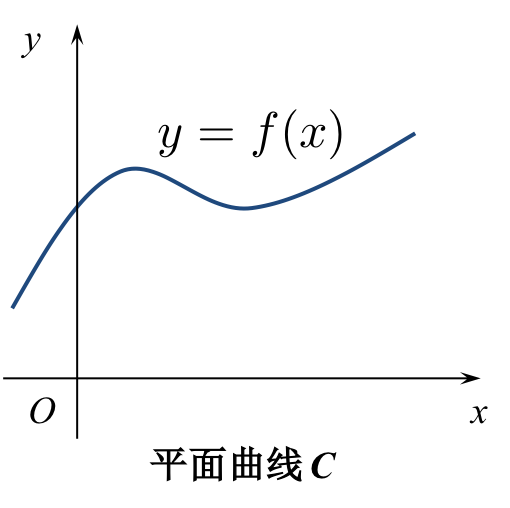
\includegraphics[width=\marginparwidth]{./images/Ch01/yfx.png}}
$$G=\{(x,f(x))\in\mathbb{R}^2|x\in D\}.$$

{\bf 思考:}一元函数的图像是否一定是平面内的一条曲线?

\ifhint
答:不一定,有可能是完全不连续的形态,不构成任何一段曲线。例如:
稍后将要介绍的Diriclet函数(在有理数点和无理数点上分别取值$0$和$1$)。
\fi

\begin{shaded}
	在微积分这门课中,我们还将学习:

	{\it 多元($n$元)函数}, 形如
	$$f:D\to\mathbb{R},\quad D\in\mathbb{R}^n\quad
	\mbox{或}\quad y=f(\bm{x}),\;\bm{x}\in D\subset\mathbb{R}^n$$

	{\it ($n$维)向量值函数,}形如
	$$\bm{f}:D\to\mathbb{R}^n,\quad, D\in\mathbb{R}\quad
	\mbox{或}\quad \bm{y}=\bm{f}(x),x\in D\subset\mathbb{R},
	\bm{y}\in\mathbb{R}^n$$
		
	{\bf 思考:}二元函数和三维的向量值函数可以表示怎样的几何对象?
	\ifhint
	\pss{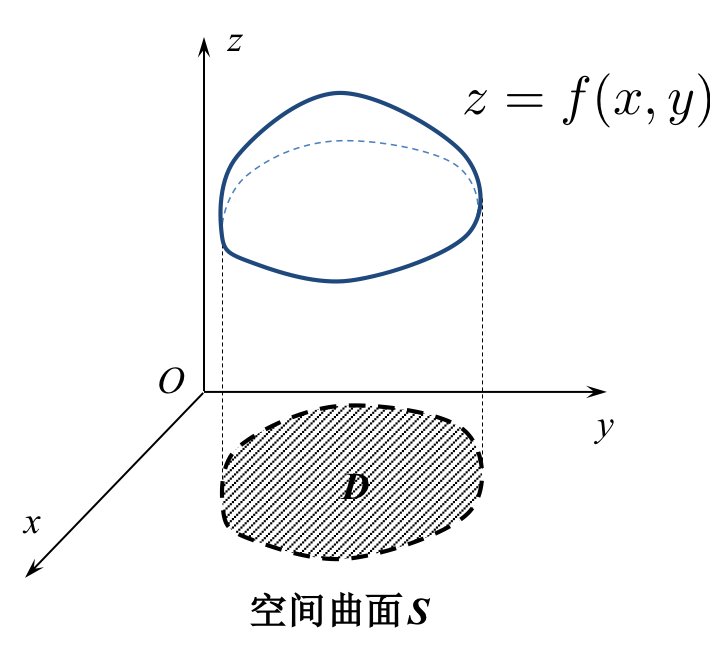
\includegraphics[width=\marginparwidth]{./images/Ch01/zfxy.png}}
	二元函数的图像一般可以表示为三维空间中的一个曲面,而三维的向量值
	函数则对应于三维空间中的一条曲线。
	\fi
\end{shaded}
	
{\bf 思考:}平面曲线与一元函数具有一一对应关系吗?空间曲面和二元函数呢?

\ifhint
答:不是的,例如圆$x^2+y^2=1$如果写成一元函数形式,需要至少两个函数
$y=\pm\sqrt{1-x^2}$。空间曲面和二元函数的关系与之类似,例如空间球面
$x^2+y^2+z^2=1$也至少需要写成两个$z$关于$x,y$的二元函数
$z=\pm\sqrt{1-x^2-y^2}$。
	
由于以上问题的存在,为了表示平面曲线(空间曲面),我们会用到其他一些的曲线方程,
例如:单位圆的方程也可以写为:
\begin{itemize}
	\item {\it 隐函数方程}:$x^2+y^2=1$;
	\item {\it 参数方程}:$(x,y)=(\cos t,\sin t),\quad t\in[0,2\pi]$;
	\pss{关于参数方程和极坐标方程的介绍,参见KD教材1.3节}
	\item {\it 极坐标方程}:$\rho=1,\theta\in[0,2\pi]$。
\end{itemize}
\fi
	
\subsubsection{函数的运算}

函数运算是由基本函数构造更复杂函数的常用手段,常见的函数运算包括:
\begin{enumerate}
  \setlength{\itemindent}{1cm}
  \item {\it 四则运算:}$+,-,\cdot,/$;
  \item {\it 复合运算:}函数的复合运算就是
  中间变量的代入过程,可表示为:$(f\circ g)(x)=f(g(x))$;
  \item {\it 逆运算:}也就是求反函数。
  \ps{函数求逆(反函数)的前提:$f$必须为一一映射}。
\end{enumerate}

\bs
{\bf 思考:}$y=f(x)$和$x=f^{-1}(y)$的图形的关系是怎样的?

\ifhint
答:相同!
\fi

\subsubsection{函数的简单性质}

今后的讨论中,为了书写方便,我们约定可使用如下的简写符号:
\begin{tcolorbox}[colback=white!90!black]
	{\bf 常用的简写符号:}约定用于数学推导中一些常用文字的书写替代,汉英通用
	\begin{itemize}
	  \item[{\b$\bm{\forall}$}]  \quad 任意 (for all, arbitrary)
	  \item[{\b$\bm{\exists}$}] \quad 存在 (exist)
	  \item[{\b$\bm{\Rightarrow}$}] \quad 推出 (deduce, imply)
	  \item[{\b$\bm{\Leftrightarrow}$}] \quad 等价、当且仅当 (equivalent, if and only if)
	  \item[{\b$\bm{\to}$}] \quad 趋于 (approach)
	\end{itemize}
\end{tcolorbox}

{\bf 1.有界性}

设$I\subset\mathbb{R}$,$f(x)$在$I$上有定义,若集合
$\{f(x)|x\in I\}$有界,
则称{\bf $f(x)$在$I$上有界}或{\bf $f(x)$是$I$上的有界函数}。
\ps{函数有界就是其值域有界}

\bs
\egz 判断以下函数在其定义域上的有界性\ps{参见图\ref{fig:sinFigures}}

\quad(1)\;$y=x\sin x$,\hspace{5em} (2)\;$y=\df{\sin x}x$,
\hspace{5em} (3)\;$y=\sin\df1x$

\begin{figure}[h]
	\centering
	\begin{subfigure}[t]{0.45\textwidth}
		\centering
		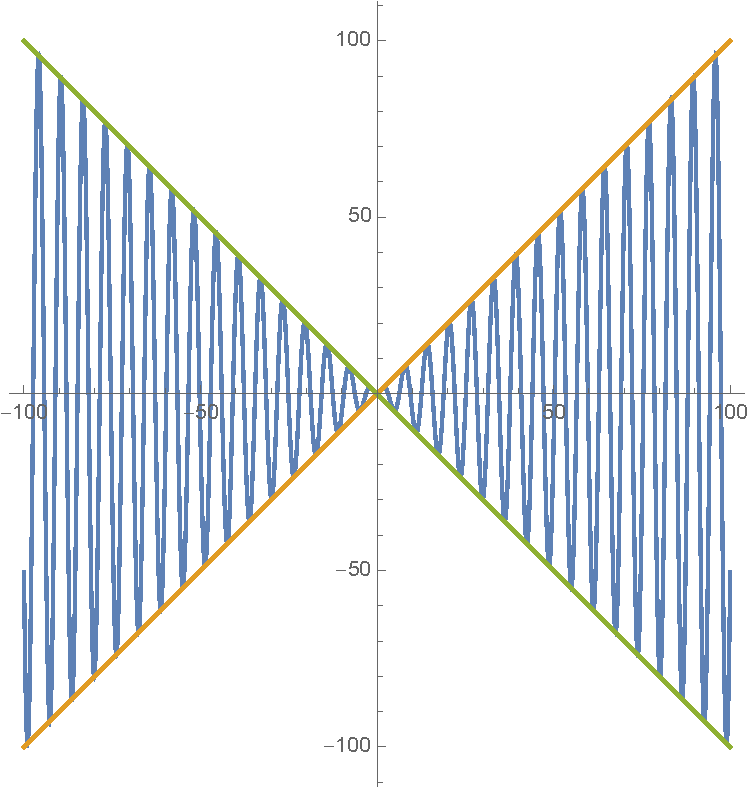
\includegraphics[width=\textwidth]{./images/Ch01/xsinx.pdf}
		\caption{$y=x\sin x$}
	\end{subfigure}

	\begin{subfigure}[t]{0.45\textwidth}
		\centering
		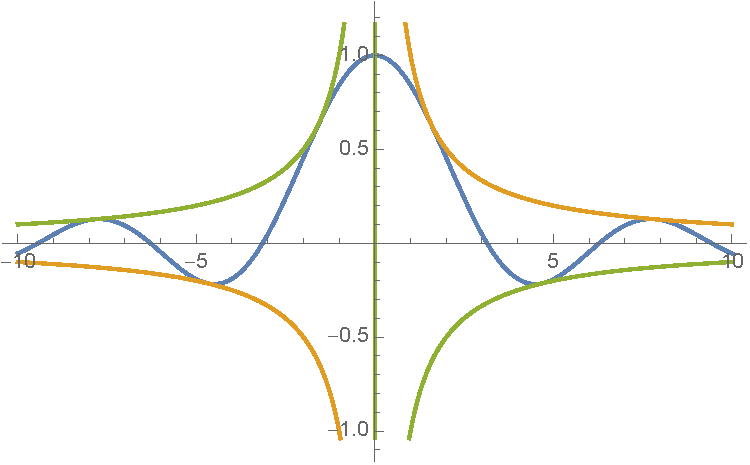
\includegraphics[width=\textwidth]{./images/Ch01/1xsinx.pdf}
		\caption{$y=\df{\sin x}x$}
	\end{subfigure}\quad
	\begin{subfigure}[t]{0.45\textwidth}
		\centering
		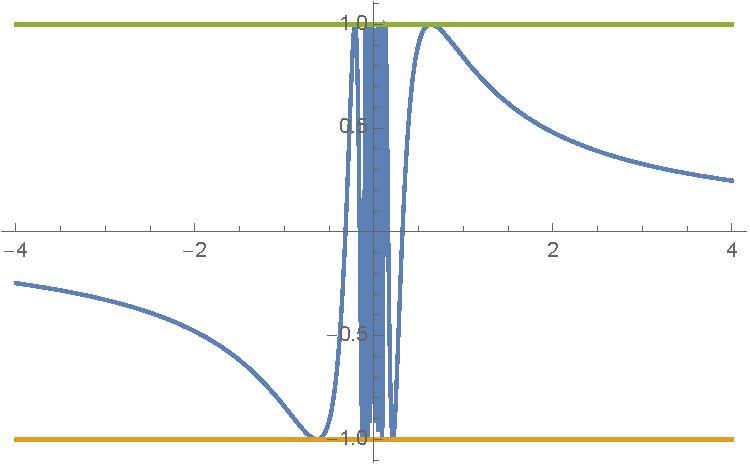
\includegraphics[width=\textwidth]{./images/Ch01/sin1x.pdf}
		\caption{$y=\sin\df1x$}
	\end{subfigure}
	\caption{\exNo 图(建议熟练掌握)}
	\label{fig:sinFigures}
\end{figure}

\begin{shaded}
	{\bf 反(否)命题的写法}	

	有时候,我们已经需要给出某个命题的反(否)命题。根据一阶逻辑的基本
	法则,可以得到如下的替换规则:逐个对命题中的如下文字进行相互替换
	\begin{enumerate}
	  \setlength{\itemindent}{1cm}
	  \item {\b “任意”与“存在”}
	  \item {\b “$\geq(\leq)$”与“$<(>)$”}
	  \item {\b “和”与“或”}
	\end{enumerate}
	
	\bs
	以函数的有界性为例,其否命题为函数无界。
	\begin{tcolorbox}
		{\it $f(x)$在区间$I$上有上界}:{\b\it 存在}$M\in\mathbb{R}$,对
		{\b\it 任意}$x\in I$,有$f(x){\b \leq} M$。
		
		{\bf $f(x)$在区间$I$上无上界}:对{\b\it 任意}$M\in\mathbb{R}$,
		{\b\it 存在}$x_M\in I$,使得$f(x_M){\b >}M$。
	\end{tcolorbox}
	
	\bs
	\egz 用以上关于函数无上界的定义,证明$y=x\sin x$无界。
	
	注:所谓{\it 用定义证明}函数的性质,就是验证该函数满足这个定义中的命题。
	
	证:对任意$M\in\mathbb{R}$,
	令$x_M=\left(\left[\df{M}{2\pi}\right]+1\right)
	\cdot2\pi+\df{\pi}2$(其中$[x]$为{\it 下取整函数},表示不大于$x$的最大整数,
	显然$[x]\leq x<[x]+1$),	则有
	$$x_M>\df{M}{2\pi}\cdot2\pi+\df{\pi}2>M,
	\quad\mbox{且}\quad \sin x_M=1,$$
	故
	$$x_M\sin x_M=x_M>M.$$
	从而根据函数无上界的定义,可知该函数无上界,从而无界。\fin
	
	注:有界是指既有上界又有下界,故无上界或无下界都可推出无界!
	
	\bs
	\egz 证明:$f(x)=\df{\cos x}x$无界。
	
	证:对任意$M>0$,令$x_M=\min\left\{\df{\pi}4,\df1{2M+1}\right\}$,
	由于$x_M<\pi/3$时,$\cos x_M>\df12$,故
	$$f(x_M)>\df1{2x_M}\geq\df1{2\df1{2M+1}}=M+\df12>M,$$
	于是由定义可知,$f(x)$无界。\fin
\end{shaded}		

{\bf 思考:}设$a,b$为常数,证明函数
$$f(x)=|x-a|-|x-b|$$
有界。

\ifhint
提示:给出函数的分段定义,再观察即可。
\fi

{\bf 2.单调性}

设$f:I\mapsto\mathbb{R}$,若对$\forall x_1,x_2\in I$,总有
$$x_1<x_2\Rightarrow f(x_1)\leq f(x_2)$$
则称{\bf $f(x)$在$I$上单调递增}(若不等式中的等号总是无法成立,则称为
{\bf 严格单调递增})
	
\bs
\egz 证明函数$f(x)=x+\sin x$严格单调递增。
\ps{\centering
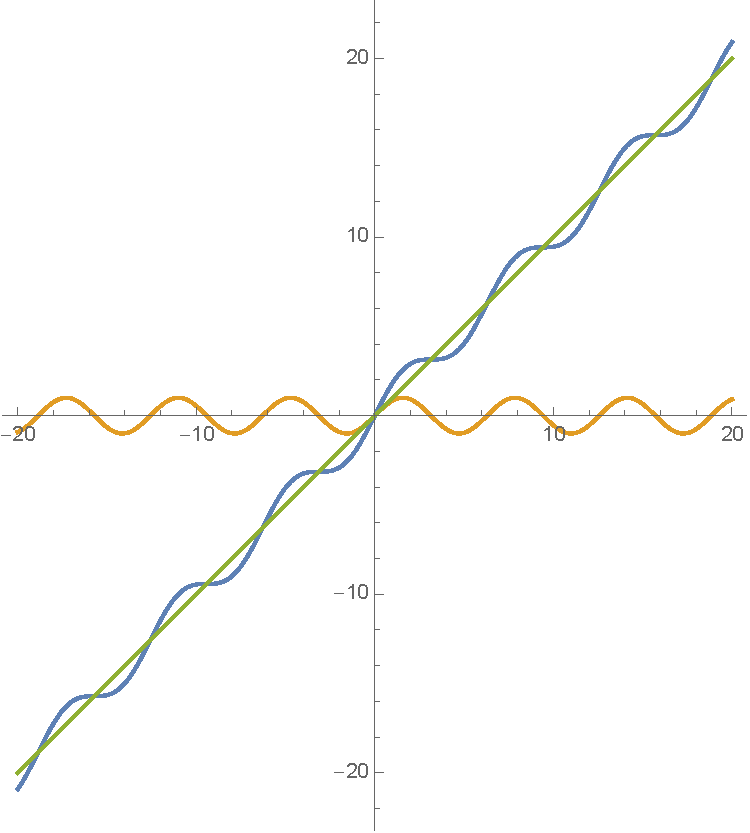
\includegraphics[width=\marginparwidth]{./images/ch01/xpsinx.pdf}\\
$y=x+\sin x$和$y=\sin x$}

证:该函数的定义域为$\mathbb{R}$,任取$x_1,x_2\in\mathbb{R}$,则
$$f(x_2)-f(x_1)=(x_2-x_1)+2\sin\df{x_2-x_1}{2}\cos\df{x_2+x_1}{2}.$$

若$x_2-x_1>2\pi$,则由$\sin\df{x_2-x_1}{2}\cos\df{x_2+x_1}{2}\geq -1$,可得
$$f(x_2)-f(x_1)>(x_2-x_1)-2>2\pi-2>0;$$

若$0<x_2-x_1<2\pi$,注意到$|\sin x|<x\;(x>0)$,则有
$$f(x_2)-f(x_1)>(x_2-x_1)-2\left|\sin\df{x_2-x_1}{2}\right|
>(x_2-x_1)-2\df{x_2-x_1}{2}=0.$$

综上所述,对任意$x_2>x_1$,恒有$f(x_2)-f(x_1)>0$,故$f(x)$严格单调递增。
\fin

\bs
{\bf 思考:}严格单调的函数一定是一一映射,故一定存在反函数。如果反之,
存在反函数的函数一定会严格单调吗?

\ifhint
答:反之不成立。例如函数
\ps{\centering
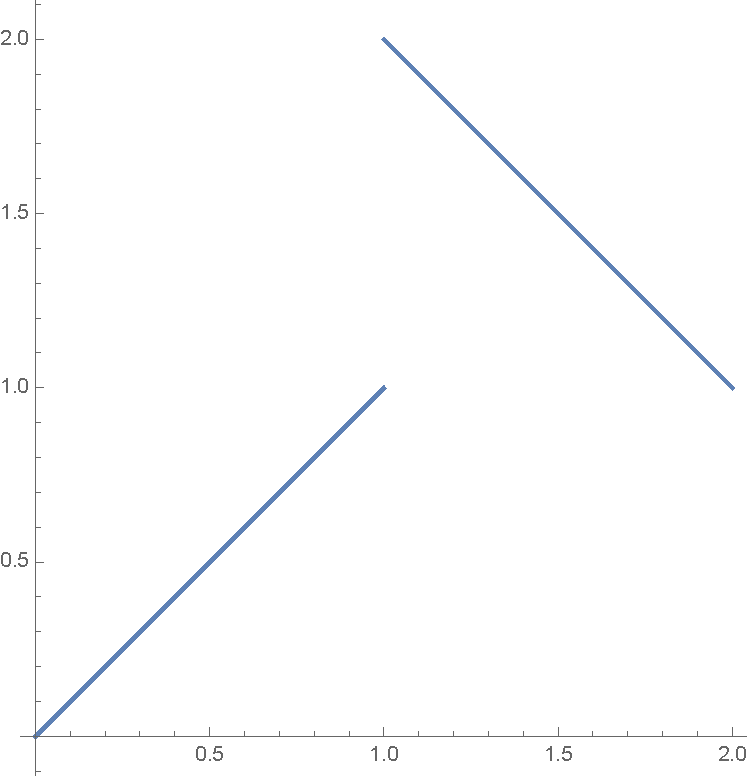
\includegraphics[width=0.9\marginparwidth]{./images/ch01/pswsRef.pdf}\\
可逆但不整体单调}
$$f(x)=\left\{\begin{array}{ll}
	x,&0<x<1;\\
	3-x,&1\leq x<2
\end{array}\right.$$
的反函数就是其自身,但在定义域上不是单调的。\fin

请进一步思考:以上反例中的函数在每个连续的区间(例如$(0,1)$)
上仍然是严格单调的,这是函数存在反函数的必要条件吗?换句话说,
是否存在某个函数存在反函数,却在任意的区间上都不单调呢?
\fi

\bs
{\bf 思考:}若对任意$x_1,x_2$,总有
$$[f(x_2)-f(x_1)](x_2-x_1)\leq 0,$$
可以推断$y=f(x)$具有何种性质?

\ifhint
答:$y=f(x)$单调递减。
\fi

\bs
{\bf 思考:}设$f(x),g(x)$均为区间$(a,b)$上的增函数,证明函数
\begin{align*}
	\varphi(x)&=\max_{x\in(a,b)}\{f(x),g(x)\}\\
	\psi(x)&=\min_{x\in(a,b)}\{f(x),g(x)\}
\end{align*}
均为$(a,b)$上的增函数。

\ifhint
提示:根据$f(x),g(x)$在特定点上的取值大小关系进行讨论。

例如,设$x_2>x_1$,且$f(x_2)\leq g(x_2),f(x_1)\geq g(x_1)$,则
$$\varphi(x_2)-\varphi(x_1)
=g(x_2)-f(x_1)\geq f(x_2)-f(x_1)\geq 0.$$
\fi

\bs
{\bf 思考:}设$\frac{f(x)}x$在$(0,+\infty)$上单调递减,证明:
对任意$x>0,y>0$,均有
$$f(x+y)\leq f(x)+f(y).$$

\ifhint
提示:$\frac{f(x)}x$在$(0,+\infty)$上单调递减,故对任意
$x_1\geq x_1>0$,均有
$$\frac{f(x_2)}{x_2}\leq \frac{f(x_1)}{x_1},$$
进而
$$f(x_2)\leq f(x_1)\df{x_2}{x_1}.$$
不妨设$x\leq y$,则
$$f(x+y)\leq f(x)\df{x+y}x,\quad
f(x)\df yx\leq f(y),$$
于是
\begin{align*}
	f(x+y)-f(x)
	\leq f(x)\left(\df{x+y}x-1\right)
	=f(x)\df yx\leq f(y).
\end{align*}
\fi

\bs

{\bf 3.奇偶性}

设函数$f:D\mapsto\mathbb{R}$,{\bf 称$f(x)$为偶(奇)函数},是指:
对任意$x\in D$,有$f(-x)=f(x)\quad(f(-x)=-f(x))$

奇偶性是对称性的一种特例,由奇偶性的定义,很容易得到关于函数对称性的一些定义:

\bs
\egz 试给出如下性质的数学定义
\begin{enumerate}[(1)]
  \setlength{\itemindent}{1cm}
  \item 函数$y=f(x)$的图像关于$x=a$对称
  \dotfill$f(2a-x)=f(x)$
  \item 函数$y=f(x)$的图像关于点$(x_0,y_0)$对称
  \dotfill $f(2a-x)=2f(a)-f(x)$
\end{enumerate}

\bs
{\bf 思考:}$f(x)=g(a-x),\;(x\in\mathbb{R})$有什么几何意义?

\ifhint
答:$f(x)$和$g(x)$的图像关于$x=a/2$对称!例如:$\sin x
=\cos(\pi/2-x)$,函数$y=\sin x$和$y=\cos x$图像关于$x=\pi/4$对称。
\fi

\bs
\begin{thx}
	{\bf 定理:}任意一个定义在对称区间上的函数均可以表示为一个偶函数和一个奇函数的和,即
	$$f(x)=\df{f(x)+f(-x)}{2}+\df{f(x)-f(-x)}{2}.$$
\end{thx}
例如:
$$e^x=\df{e^x+e^{-x}}2+\df{e^x-e^{-x}}2$$

\bs
{\bf 4.周期性}

设函数$f:\mathbb{R}\to\mathbb{R}$,
称{\bf $f(x)$为周期函数},是指: 存在$T>0$,
使对任意$x\in\mathbb{R}$,有
$f(x+T)=f(x)$。
满足以上性质的最小正数$T$称为$f(x)$的{\bf 最小正周期}。
		 
显然,若$T$为$f(x)$的一个周期,则任意$n\in\mathbb{Z}$和
任意$x\in\mathbb{R}$,总成立
$$f(x+nT)=f(x).$$

\bs
\egz 设定义在$(-\infty,+\infty)$上的函数$f(x)$
的图形关于直线$x=a$和$x=b$($a\ne b$)对称,证明$f(x)$
是周期函数。

证:$f(x)$的图形关于$x=a$和$x=b$对称意味着,对任意
$x\in(-\infty,+\infty)$,均有
$$f(x)=f(2a-x)=f(2b-x),$$
进而,对任意$x\in(-\infty,+\infty)$,
$$f(x)=f(2a-x)=f(2b-(2a-x))=f(2(b-a)+x),$$
因为$b-a\ne0$,故上式说明$f(x)$是以$2(b-a)$为周期的周期函数。\fin

\bs
{\bf 思考:}设$f(x)$定义在$(-\infty,+\infty)$上,且
存在$T\ne 0$,使对任意$x\in(-\infty,+\infty)$,总有
$$f(x+T)=-f(x),$$
证明:$f(x)$是周期函数。

\ifhint
提示:$f(x+2T)=-f(x+T)=f(x)$.
\fi

\bs
{\bf 思考:}设$\alpha$为无理数,证明:$\sin x+\sin\alpha x$
不是周期函数。

\ifhint
提示:用反证法。假设该函数为周期函数,$T>0$为其周期。
于是
$$\sin(T+x)+\sin\alpha(T+x)=\sin x+\sin\alpha x,$$
利用和差化积,可化为
$$\cos(T+2x)\sin T+\cos\alpha(T+2x)\sin\alpha T=0.$$
在上式中分别令$x=0$和$x=\pi$,可得
\begin{align*}
	\sin2T+\sin\alpha T\cos\alpha T=0,
	\quad
	\sin2T+2\cos\alpha(T+\pi)\sin\alpha T=0.
\end{align*}
从而可推出
$$\cos\alpha T=\cos(\alpha T+2\alpha\pi),$$
因为$\alpha$为无理数,故$2\alpha\pi$不可能是$\cos x$
的周期,从而可知上式必不成立。至此,可知假设错误。
\fi

\subsubsection{常用函数}

{\bf 1.符号函数}

$$\mathrm{sgn}\,x =\left\{
\begin{array}{rl}
-1,\;&x<0 \\
0,\;&x=0 \\
1,\;&x>0
\end{array}
\right.$$
显然,
$$|x|=x \cdot\mathrm{sgn} x$$
	
{\bf 2.(下)取整函数(阶梯函数)}

$$y=\left[ \,x\, \right]$$
其中$[\,x\,]$表示小于等于$x$的最大整数。容易得到如下的性质:
\begin{enumerate}[(1)]
  \setlength{\itemindent}{1cm}
  \item $[x]\leq x<[x]+1$
  \item $[x+1]=[x]+1$
\end{enumerate}

\bs
利用取整函数,可以构造出一些简单但在工程实践中非常重要的函数,例如:
{\it 方波}和{\it 三角波}\ps{经常也写为$y=\df1{\pi}\arccos(\cos\pi x)$}:
\begin{figure}[h]
	\centering
	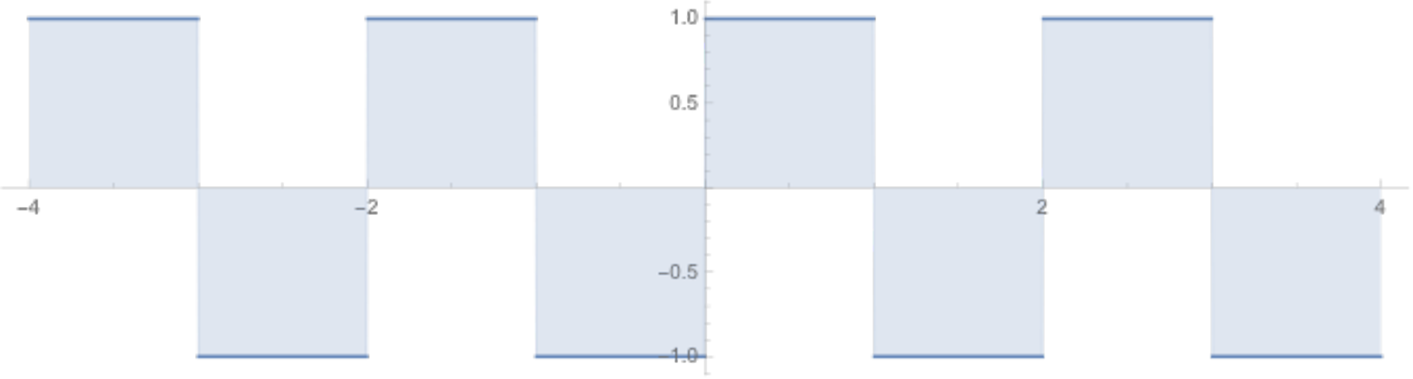
\includegraphics[width=0.7\textwidth]{./images/ch01/rectWave.pdf}
	\caption{方波$y=(-1)^{[x]}$}
	\label{fig:rectWave}
\end{figure}
\begin{figure}[h]
	\centering
	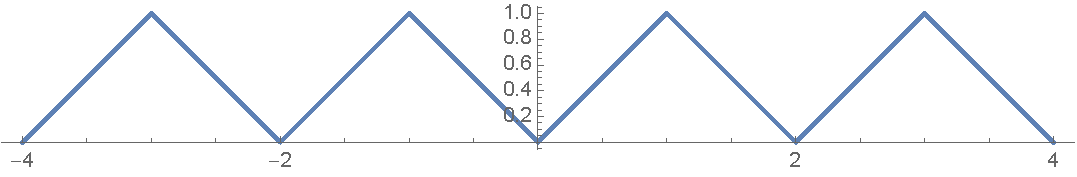
\includegraphics[width=0.7\textwidth]{./images/ch01/triWave.pdf}
	\caption{三角波$y=\left|x-2\left[\df x2\right]\right|$}
	\label{fig:triWave}
\end{figure}

\bs

{\bf 3.Dirichlet函数}

  $$\bm{D}(x) =\left\{
  \begin{array}{ll}
  	1,\;& x\in\mathbb{Q} \\
  	0,\;& x\notin\mathbb{Q}
  \end{array}
  \right.$$

  {\bf 性质:}\ps{将在后续章节中加以证明}
  \begin{enumerate}[(1)]
    \setlength{\itemindent}{1cm}
    \item $D(x)$在实数轴上处处无极限;
	\item $D(x)$在实数轴上处处不连续;
	\item {\it 仅在$x=0$这一点连续的函数:}$y=xD(x)$;
	\item {\it 仅在$x=0$这一点可导的函数:}$y=x^2D(x)$。
  \end{enumerate}

$D(x)$的最后这两个性质有些违反我们的直觉,因为现实中并不存在什么曲线
能够只在一个点连续或者只在一个点处光滑!这真是数学自身的
特异指出,为了确保自身的严谨,而适当地“牺牲”了一些与直觉
一致的东西。

\bs

{\bf 4.Riemann函数} \ps{也被称为“直尺函数”,最初由卡尔$\cdot$托梅提出}:
设$x\in[0,1]$,
  $$\bm{R}(x) =\left\{
	\begin{array}{ll}
	1,\;&x=0\\
	\displaystyle\frac 1q,\;&x=\displaystyle\frac pq,\,p,q\mbox{互素}\\
	0,\;&x\notin\mathbb{Q}
	\end{array}
  \right. $$
$R(x)$和$D(x)$一样,也有许多“反直觉”的地方,例如:
\begin{itemize}
	\item 对任意$x_0\in[0,1]$, $\lim\limits_{x\to x_0}R(x)=0$;
	\item $R(x)$在{\it 所有的无理数点处连续,在所有的有理数点处不连续};
	\item $R(x)$是Riemann可积的。
\end{itemize}

\bs

{\bf 5.初等函数}

{\bf 初等函数}
\pss{注意两个重要的限定词:
\begin{itemize}
	\item 有限次
	\item 一个式子
\end{itemize}
因此,通常来说,分段定义的函数不能算初等函数
}
是指由常数和{\it 基本初等函数}经过
{\it 有限次}的四则运算和{\it 有限次}的函数复合
步骤所构成并可用{\it 一个式子}表示的函数。

{\bf 基本初等函数}包括以下五类:
\begin{enumerate}
  \setlength{\itemindent}{1cm}
  \item {\bf 幂函数:} $y=x^a,\; (a\in\mathbb{R})$
  \item {\bf 指数函数:} $y=a^x,\; (a>0,a\ne 1)$
  \item {\bf 对数函数:} $y=\log_ax,\; (a>0,a\ne 1)$
  \item {\bf 三角函数:} $\sin x, \,\cos x,\, \tan x, \,\cot
  x,\, \sec x,\, \csc x$
  \item {\bf 反三角函数} :
  $\arcsin x, \,\arccos x, \arctan x,\ldots$
\end{enumerate}

{\baa 学习要求:熟练掌握五类基本初等函数的定义、图像、基本性质、
各种运算公式(例如:三角函数的和差化积、积化和差、半(倍)角公式、
万能公式;反三角函数的定义域、值域、单调性;一些常用的不等式,
如$e^x-1>x>\ln(x+1)\;(x>0)$、平均值不等式、
$\sin x<x<\tan x\;(x>0)$等等。}

\bs
{\bf 问:}$\arcsin x$和$\arccos x$的定义域值域有何不同?

答:因为三角函数都是周期函数,所以只能选择其周期内某个单调区间上
的一段函数来定义反函数。在选择这样的区间时,注意掌握两个原则:
(1)尽可能靠近原点;(2)有限考虑对称区间或原点右侧的区间。
常用的反三角函数的图像见图\ref{fig:triFunc}。

\begin{figure}[h]
	\centering
	\begin{subfigure}[t]{0.45\textwidth}
		\centering
		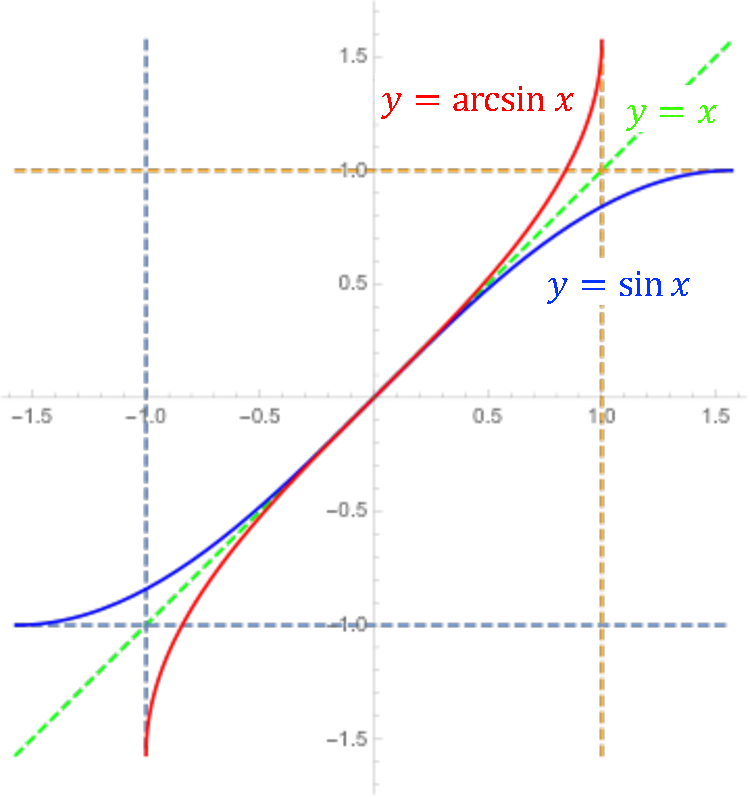
\includegraphics[width=\textwidth]
		{./Images/Ch01/sin-Arcsin.pdf}	
		\caption{$\sin x$与$\arcsin x$的图像}
	\end{subfigure}
	\begin{subfigure}[t]{0.45\textwidth}
		\centering
		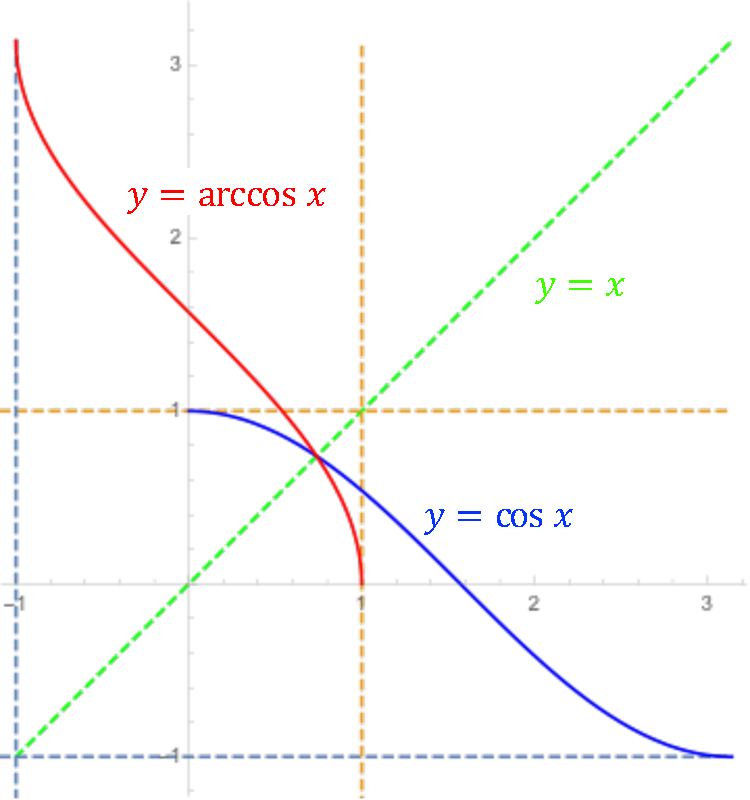
\includegraphics[width=\textwidth]
		{./Images/Ch01/cos-Arccos.pdf}	
		\caption{$\cos x$与$\arccos x$的图像}
	\end{subfigure}

	\begin{subfigure}[t]{0.45\textwidth}
		\centering
		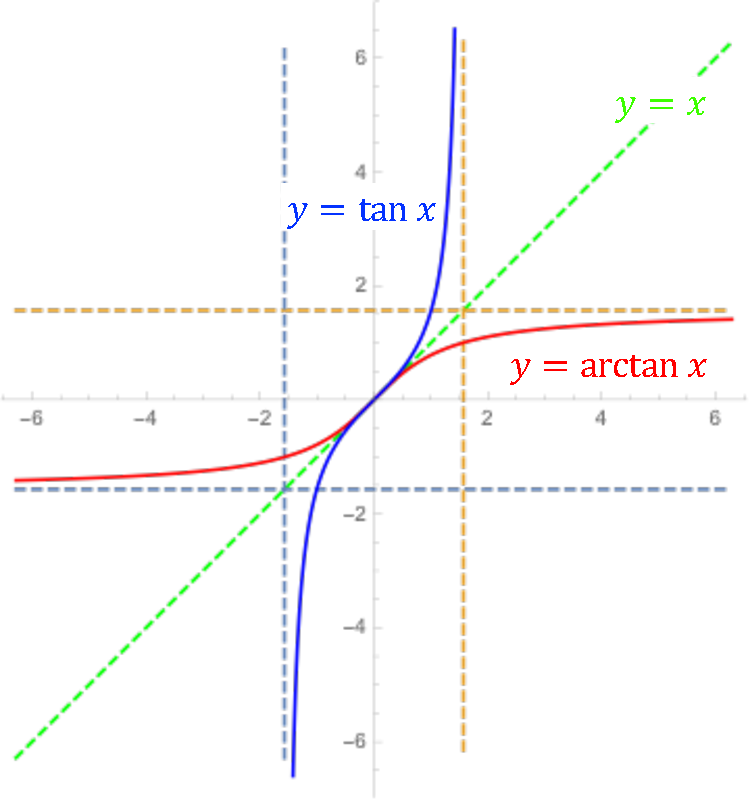
\includegraphics[width=\textwidth]
		{./Images/Ch01/tan-Arctan.pdf}	
		\caption{$\tan x$与$\arctan x$的图像}
		\label{subfig:arctan}
	\end{subfigure}
	\begin{subfigure}[t]{0.45\textwidth}
		\centering
		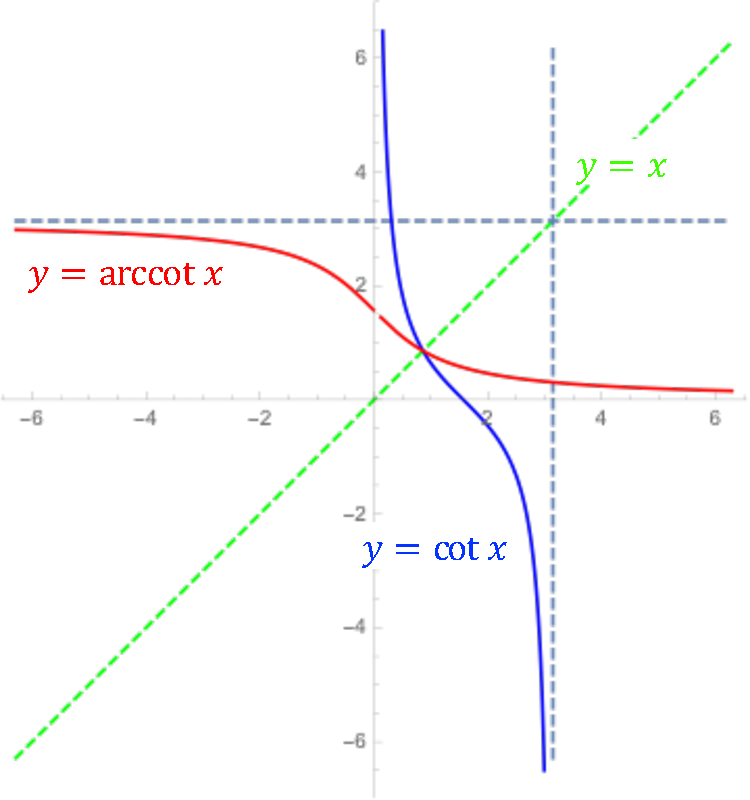
\includegraphics[width=\textwidth]
		{./Images/Ch01/cot-Arccot.pdf}	
		\caption{$\cot x$与$\mathrm{arccot} x$的图像}
	\end{subfigure}
	\caption{三角函数及其反函数的图像}
	\label{fig:triFunc}
\end{figure}

\bs
\egz 写出以下两个函数的表达式
$$\arcsin(\sin x),\quad \sin(\arcsin x)$$

解:$\sin(\arcsin x)=x$,其定义域为$[-1,1]$。

$\arcsin x$的值域为$[-\pi/2,\pi/2]$,因此作如下的讨论:

若$x\in[-\pi/2,\pi/2]$,则$\arcsin(\sin x)=x$;

若$x\notin[-\pi/2,\pi/2]$,则需要利用$\sin x$的性质
将$\sin x$化为某个$\sin(\bar x)$,其中$\bar x\in[-\pi/2,\pi/2]$,
且与$x$之间相差$\pi$的整数倍。进一步讨论:

若$\bar x-x=2n\pi$,其中$n$为整数,则$\sin\bar x=\sin x$,
此时
$$\arcsin(\sin x)=\arcsin(\sin\bar x)=\bar x=x+2n\pi.$$

若$\bar x-x=(2n+1)\pi$,其中$n$为整数,则$\sin(-\bar x)
=-\sin\bar x=\sin x$,
此时
$$\arcsin(\sin x)=\arcsin(\sin(-\bar x))=-\bar x=-(2n+1)\pi-x.$$

又注意到$\arcsin(\sin x)$显然是以$2\pi$
为周期函数,故以下只需给出其在一个周期上的
定义,其余部分按照周期进行复制即可。综上
$$\arcsin(\sin x)=\left\{\begin{array}{ll}
-x-\pi, & -\pi\leq x<-\pi/2,\\
x, & -\pi/2\leq x\leq\pi/2,\\ 
-x+\pi, & \pi/2<x\leq\pi.
\end{array}\right.$$
其图像如下
\begin{figure}[h]
	\centering
	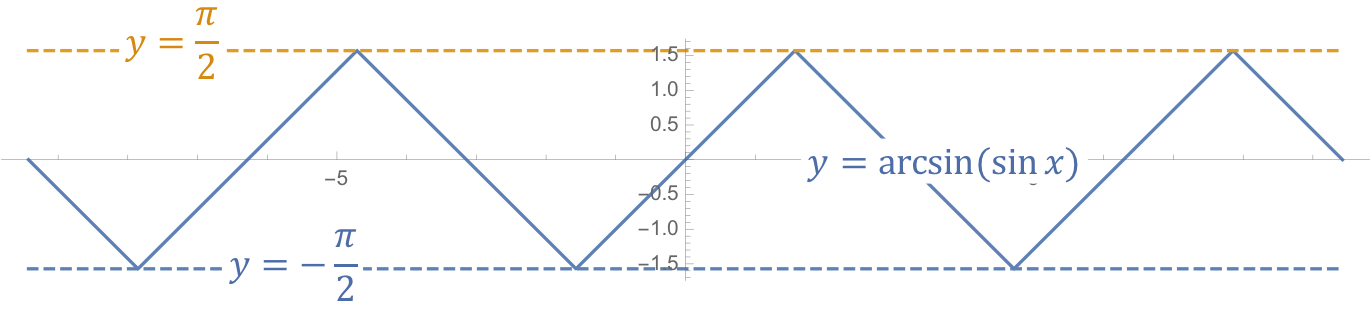
\includegraphics[width=0.7\textwidth]{./Images/Ch01/arcsin-sin.png}
	\caption{$\arcsin(\sin x)$的图像}
	\label{fig:arcsin-sin}
\end{figure}

类似地,我们可以得到$\arccos(\cos x)$的图像(如图\ref{fig:arccos-cos})\ps{请自行练习推导函数表达式}.
\begin{figure}[h]
	\centering
	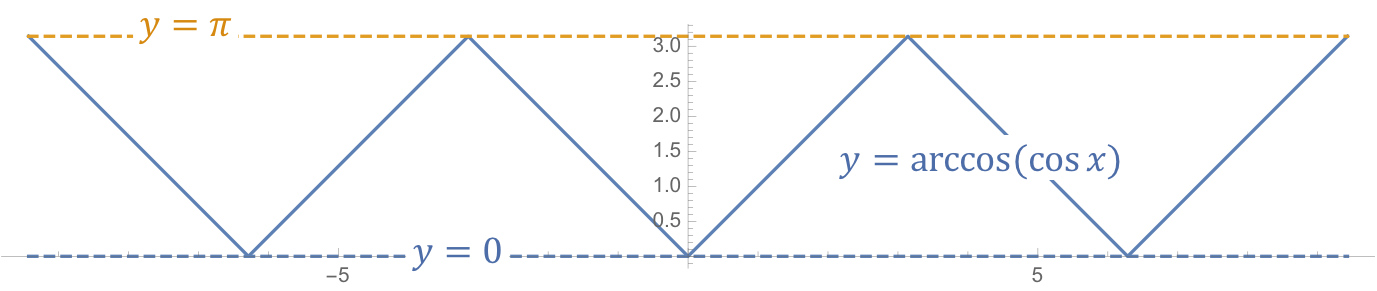
\includegraphics[width=0.7\textwidth]{./Images/Ch01/arccos-cos.png}
	\caption{$\arccos(\cos x)$的图像}
	\label{fig:arccos-cos}
\end{figure}
\fin

\egz 化简$\tan(\arcsin x),\;x\in(-1,1)$。

解:注意到
$$\tan x=\df{\sin x}{\cos x}=\df{\sin x}{\sqrt{1-\sin^2x}},$$
故
$$\mbox{原式}=\df x{\sqrt{1-x^2}},\quad x\in(-1,1).$$
\fin

{\bf 思考:}证明:$\pi=20\arctan\df17+8\arctan\df3{79}$.

\ifhint
提示:等式两边都除以$4$,然后取正切,再反复利用如下公式
$$\tan(A+B)=\df{\tan A+\tan B}{1-\tan A\tan B}.$$
\fi

\bs
{\bf 思考:}化简如下的公式
$$\arctan\df13+\arctan\df17+\ldots+\arctan\df1{n^2+n+1}$$

\ifhint
提示:
$\tan\left(\arctan\df1{n}-\arctan1{n+1}\right)=\df1{n^2+n+1}.$
\fi

\bs

{\bf 6.多项式函数}

多项式函数是一类非常“有用”的函数。之所以这么说,原因有二,一是因为
在所有的初等函数中,多项式函数是形式最简单的函数之一(只包含基本的
四则运算),因此任意给定自变量的值总可以直接计算出对应的函数值
(类似$e^x$,$\sin x$,$\arccos x$这样的函数都不行);
二是多项式函数具有很多重要的性质,使得它可以用来作为研究其他许多
函数的工具,甚至可以说,它是函数论中最重要、
最基本的工具也不为过。

一般的{\bf (一元$n$次)多项式函数}\ps{有理函数的次数也即其最高次幂
的项的次数}形如
$$P_n(x)=\sum_{i=0}^na_ix^i,
\quad (a_i\in\mathbb{R},a_n\ne 0,i=1,2,\ldots,n),$$
直观地说,它就是$x$的整数次幂的{\it 线性组合}。

多项式函数的基本性质包括\ps{这些性质的证明请参见高等代数有关的教材}:
  \begin{enumerate}[(1)]
    \setlength{\itemindent}{1cm}
    \item { $n$次多项式方程$P_n(x)=0$在$\mathbb{R}$上最多有$n$个根 (包含重根) ,在
    $\mathbb{C}$上有且仅有$n$个根(包含重根)};
    \item 设$x_i\in\mathbb{C}(i=1,2,\ldots,n)$为$P_n(x)=0$的全部根 ,则
    $$P_n(x)=a_n\prod_{i=1}^n(x-x_i)=a_n(x-x_1)(x-x_2)\ldots(x-x_n),$$
    \item 已知$P_n(x)$在$n+1$个点处的值, 可以唯一确定$P_n(x)$。
  \end{enumerate}

\bs
{\bf 思考:}证明任何正系数多项式函数$P(x)$都不可能同时满足
$P(7)=5$和$P(15)=9$。

\ifhint
提示:反证法。设
$$P(x)=\sum\limits_{k=0}^na_kx^k,$$
则
\begin{align*}
	P(15)-P(7)=\sum\limits_{k=0}^na_k\left[(15)^k-7^k\right],
\end{align*}
不难验证,对任意$k=1,2,\ldots,n$,$(15)^k-7^k$均可以被$8$整除,
因此$P(15)-P(7)$也可以被$8$整除,从而与已知矛盾。
\fi

\bs

{\bf 7.有理函数}

有理函数也叫有理(分式)函数,形如:
$$f(x)=\frac{P(x)}{Q(x)}, \quad\mbox{其中}P(x),Q(x)\mbox{均为多项式函数}$$

和多项式函数类似,有理函数也是只要给定自变量的值就可以直接计算函数值的。

关于有理函数,需要我们掌握如下的性质:任意有理函数总可以化为一个多项式
函数和一个真分式(分子的次数比分母低的有理函数)的和。例如,使用
多项式的带余除法,我们可以得到
$$\frac{x^3+x^2-1}{x-1}=x^2+2x+2+\df{1}{x-1},$$
具体的除法过程如下,类似于小学学习过的竖式除法
\begin{center}
	\polylongdiv{x^3+x^2-1}{x-1}
\end{center}

{\bf 8.双曲函数}

此类函数的在本课程中使用较少,作为了解即可。\ps{详细介绍请参见教材}

$$\sinh x =\df{e^x-e^{-x}}{2}, \quad
\cosh x =\df{e^x+e^{-x}}{2}, \quad\tanh x=\df{\sinh
x}{\cosh x}, \ldots$$

注:双曲函数在很多场合也写作$\mathrm{ch}(x)$和$\mathrm{sh}(x)$

\bigskip

\begin{ext}
	{\centering\bf 习题1-1}
	
	{\b\kaishu 说明:	今后所有的作业必须写在作业本上,作业本第一页背面上贴上一张个人的照片,
	标注专业和籍贯。作业须写明题目所在章节、题号;如非特别说明,	所有题目必须抄题;
	未作或作错的题目讲评后务必及时订正。}
	
	\begin{enumerate}  
	  %\item 证明:函数$\mathrm{arsh}\,
	  %x=\ln(x+\sqrt{x^2+1})$严格单调递增。
	  \item 证明:函数$y=x\sin x$无界。
	  \item 给出函数$y=\arcsin(\cos x)$的分段定义表达式,并画出其图像。
	  \item 试利用取整函数给出以下曲线的方程(不要写成分段函数的形式)
	  \begin{center}
	  	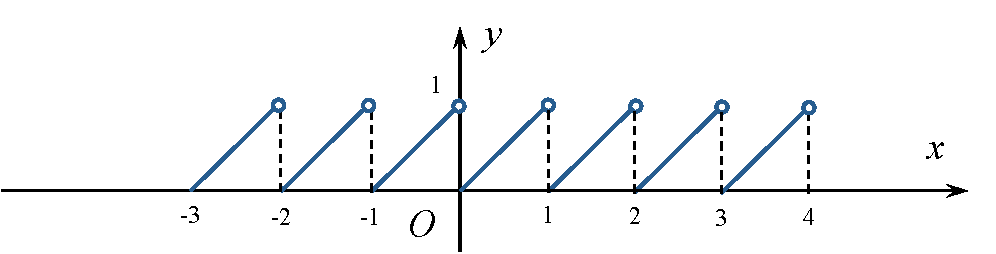
\includegraphics[width=0.7\textwidth]{./images/Ch01/f1.pdf}\\
	  	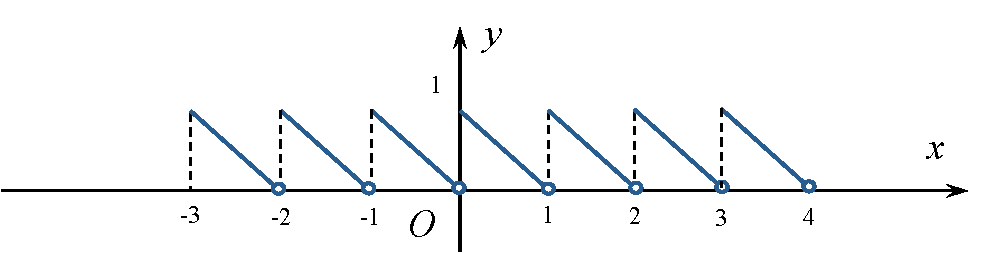
\includegraphics[width=0.7\textwidth]{./images/Ch01/f2.pdf}\\
	  	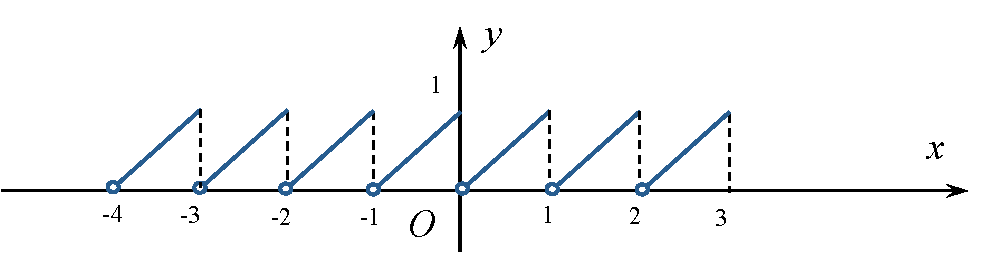
\includegraphics[width=0.7\textwidth]{./images/Ch01/f3.pdf}
	  \end{center}
	  \item 如左图,将单位圆上的点$Q$映射成数轴上的点$P$的映射称为{\it 球极投影映射},
	  请给出:
	  \begin{enumerate}[(1)]
	    \item $Q$的极角$\theta$与$P$的横坐标$x_P$的对应关系;
	    \item 将$Q$的坐标$(x_Q,y_Q)$表示为$P$的坐标$(x_P,y_P)$的函数;
	    \item 思考(选作):参考右图,给出将一个单位球面映射为二维平面的
	    {\it 三维球极投影映射},将球面上一点的坐标表示为对应二维平面
	    上的点的函数。
	  \end{enumerate}
	\begin{center}
		\resizebox{!}{5cm}{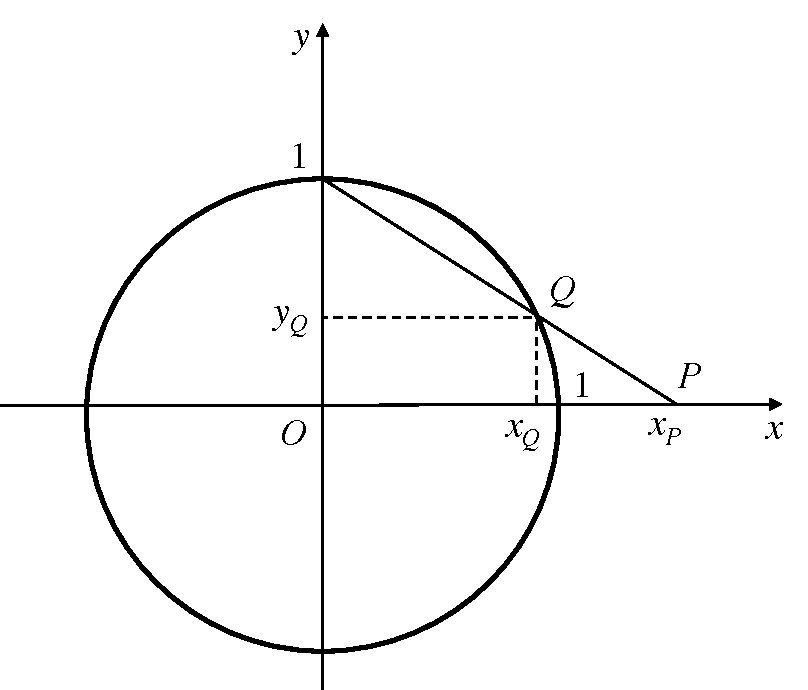
\includegraphics{./images/ch01/sphereline2D.pdf}}\quad
		\resizebox{!}{5cm}{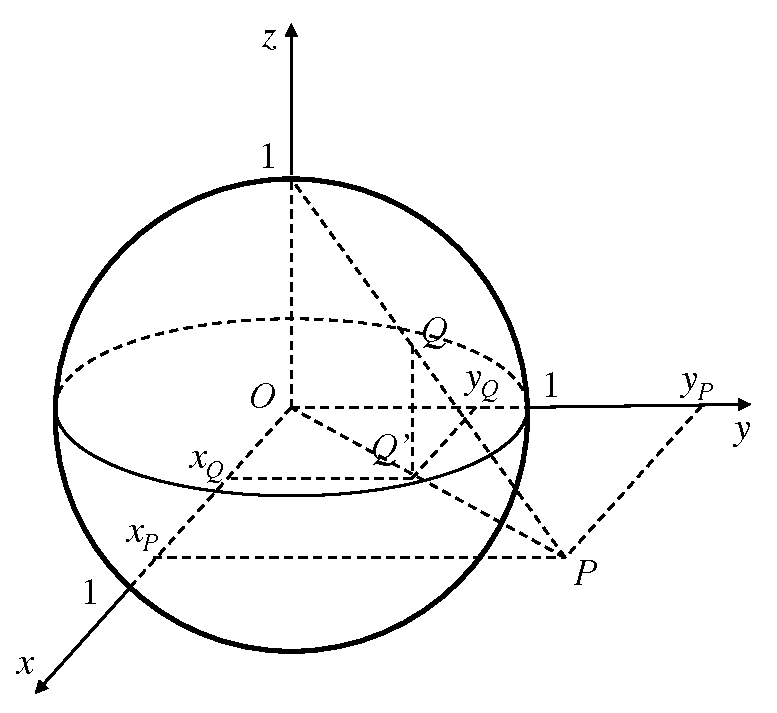
\includegraphics{./images/ch01/sphereline3D.pdf}}
		
		\it \small 第4题图
	\end{center}
%	\item (选作)对任意$x_0\in\mathbb{R}$,试给出两个数列$\{x^{(1)}_n\}$和
%	$\{x^{(2)}_n\}$,而且分别为有理数列和无理数列,且都以$x_0$为极限。
	\item (选作)以椭圆$\df{x^2}{a^2}+\df{y^2}{b^2}=1$的左焦点为极点,
	沿$x$轴正向取极轴,求该椭圆的极坐标方程。
	\end{enumerate}
\end{ext}

\section{数列的极限}

极限概念的引入是微积分发展史上具有革命性的一步,
为奠定微积分理论“无可非议”的扎实
基础提供了可能。后续我们将要学习的导数、积分、
级数等重要概念都是以极限的形式定义的。

数列极限是极限问题中最为简单的一类,也是性质非常典型的一类,
可以作为我们后续学习函数极限的基础。

\bs
{\bf 数列}就是按一定规律排列的无穷多个(相同或不相同的)数,一般记作:
\pss{\baa 有序性是数列的重要特征,
改变了数列中数的排列顺序将得到不同的数列}
$$a_1,a_2,\ldots,a_n,\ldots\quad\mbox{或者}\quad\{a_n\}.$$

$\{a_n\}$的实质是定义在$\mathbb{Z}_+$上的函数,因此数列也被称为
{\it 整标函数}或{\it 整序函数}。如果在平面直角坐标系内作图,
可以将其视为一个动点随$n$增大所留下的离散的运动轨迹。

下面是一些数列的例子:
\begin{enumerate}[(1)]
  \setlength{\itemindent}{1cm}
  \item[(1)] $\left\{\df{n+1}n\right\}:\df 21,\df 32,\df43,\df54,\df65,\ldots$
  \item[(2)] $\left\{\df{(-1)^n}n\right\}:-1,\df12,-\df13,\df14,-\df15,\df16,\ldots$
  \item[(3)] $\{n^2\}:1,4,9,16,25,36,\ldots$
  \item[(4)] $\left\{n^{(-1)^n}\right\}:1,2,\df13,4,\df15,6,\ldots$
\end{enumerate}

\bs
{\bf 思考:}数列与集合有哪些区别?

\ifhint
提示:1、有序-无序;2、无限-可能有限;3、元素可重复-元素不可重复.
\fi

\subsection{数列的极限}

形象地说,数列$\{a_n\}$的{\it 极限},
\pss{微积分中的极限概念不同于现实生活里的极限,
现实中的极限是指可能达到的最大或最小值,类似于我们所说的
上确界和下确界。例如:人类速度的极限}
就是$a_n$的值随$n$的不断增大而趋向的某个{\it 确定}的值,
当然,对于不同的$\{a_n\}$,这个确定的值不一定都存在!例如:
\begin{enumerate}[(1)]
  \setlength{\itemindent}{1cm}
  \item $\left\{\df1n\right\}$
  的值随着$n$不断增大会越来越趋近于$0$,因此其极限为$0$;
  \item $\{n\}$的取值会越来越大,甚至可以超过任何事先给定给定的值,
  因此也不会趋于任何确定的值,极限不存在;
  \item $\{(-1)^n\}$的取值在$1$和$-1$上反复交替,从整体上看,
  既不能说它趋近与$1$,也不能说它趋近于$-1$,所以极限也不存在。
\end{enumerate}

在直观理解的基础上,我们主要关注这样一个问题:{\it 在数学上如何表达这种
趋向某个确定值的特征,或者说,如何给出数列极限的数学定义?}

以下的定义由数学家Weierstrass最终完成(注意,不是发明),
\pss{现行的极限符号$\lim$据说由数学家Hardy(1877-1947)引入,
而最初提出通过引入极限来解决微积分理论不严密问题的人是
法国数学家d'Alembert}
这是被数学界最广泛接受的一种极限定义:

\begin{thx}
	对于数列$\{a_n\}$,若存在常数$a$,对任意$\e>0$(不论它有多小),
	都存在$N\in\mathbb{Z}_+$,使对任意$n>N$,都有
	$$|a_n-a|<\e$$
	成立,则称{\bf 数列$\{a_n\}$存在极限(或收敛)},
	常数$a$称为该数列的极限,记为
	$$\lim_{n\to\infty}a_n=a\quad
	\mbox{或}\quad
	a_n\to a\;(n\to\infty)$$
	若上述常数$a$不存在,则称{\bf 数列$\{a_n\}$不存在极限}(或{\bf 发散})。
\end{thx}

从几何上看(如图\ref{fig:e-N-def}所示),数列$\{a_n\}$以$a$为极限,
意味着随着$n$的增大,$a_n$可以{\it 无限}地靠近$a$。
为了表达这种“无限靠近”,数学上可以这样来解释:
对于以$a$为中心的任意小的邻域$(a-\e,a+\e)$
(图上的蓝色阴影部分),只要把$n$取得{\it 充分大}($N$的意义就是为了界定这个所谓的充分大
\ps{显然,$\e$取的越小通常意味着$N$要取的越大,
但必须注意的是$N$和$\e$
之间并不是简单的函数关系,因为如果某个$N$可以满足命题要求,
则$N$加任意的正常数显然也满足}
),则$a_n$都将落在$(a-\e,a+\e)$之内。
	
\begin{figure}[h]
	\centering
	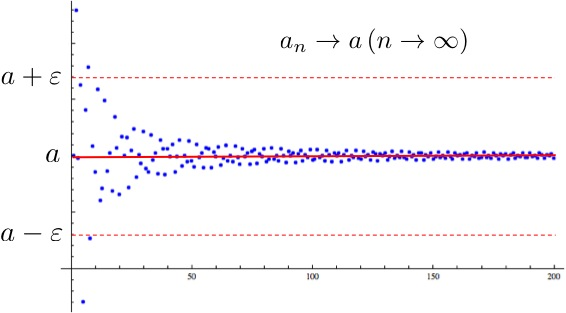
\includegraphics[width=0.45\textwidth]{./images/ch01/en1.jpg}\;
	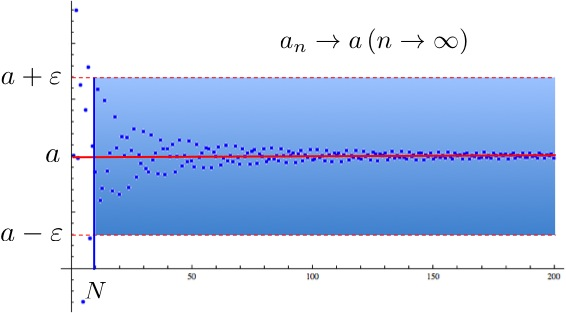
\includegraphics[width=0.45\textwidth]{./images/ch01/en2.jpg}\\
	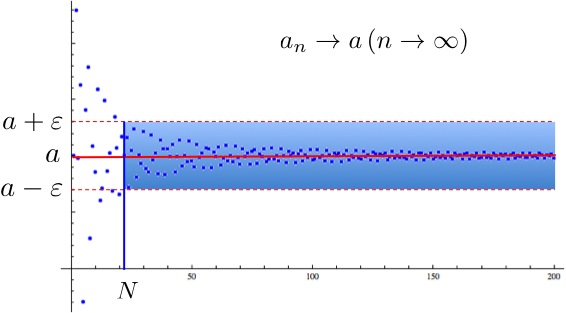
\includegraphics[width=0.45\textwidth]{./images/ch01/en3.jpg}\;
	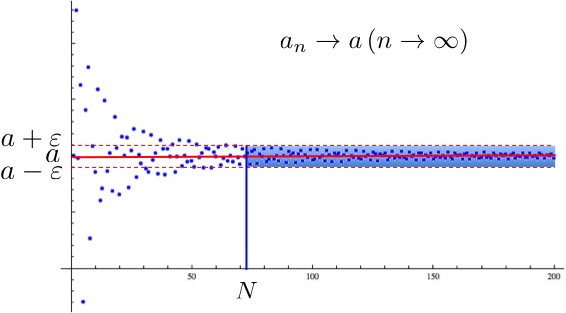
\includegraphics[width=0.45\textwidth]{./images/ch01/en4.jpg}
	\caption{不论$\e$取得多小,总存在对应的$N$,使得$n>N$对应的所有
	$a_n$都落在$U(a,\e)$之内}
	\label{fig:e-N-def}
\end{figure}

\begin{shaded}
	\pss{\centering
	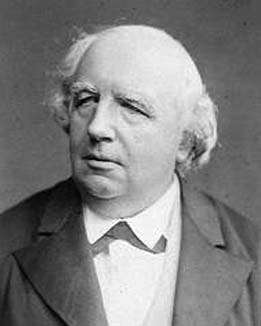
\includegraphics[width=0.7\marginparwidth]{./images/ch01/Weierstrass.jpeg}\\
	\href{https://en.wikipedia.org/wiki/Karl_Weierstrass}{K. Weierstrass(1815-1897)}\\
	 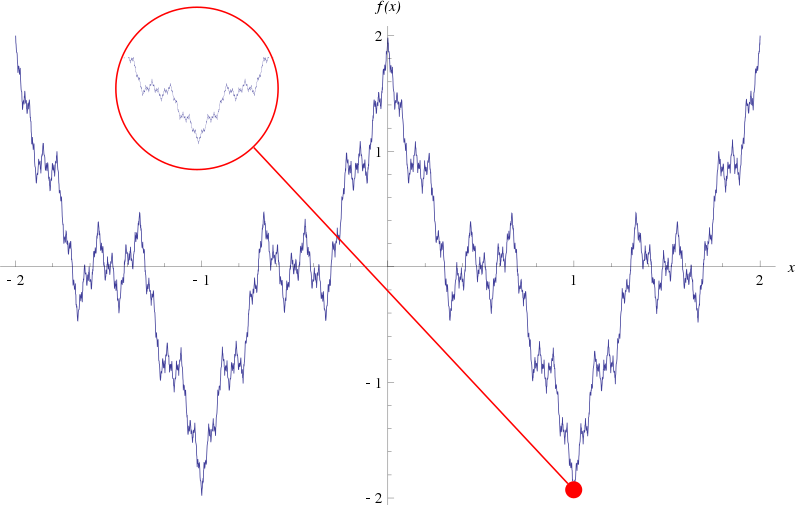
\includegraphics[width=0.7\marginparwidth]{./images/ch01/WeierstrassFunction.png}\\
	著名的\href{https://en.wikipedia.org/wiki/Weierstrass_function}
	{Weierstrass函数}
	$$f(x)=\sum\limits_{n=0}^{\infty}a^n\cos(b^n\pi x)$$
	$$\left( 0<a<1,\;ab>1+\frac32\pi\right)$$
	处处连续,但处处不可导
	}

	关于极限的定义,历史上曾经有过很长时间的讨论,当时的许多数学家都尝试
	过给出一个“合适”的极限定义,例如:Cauchy是这样描述极限的:
	
	{\kaishu
		当属于一个变量的相继值无限地趋近某个固定值时,如果以这样一种方式告终,
		变量值同固定值之差小到我们希望当任意小,那么这个固定值就成为其他所有值的极限。
	}
	
	这个定义中所描述的“趋近”这个行动,很难说是一种令人满意的表达方式。趋近是指
	一种实际的动作吗?如果是,是否意味着我们在讨论极限时,必须把时间和空间的概念
	包含在内?此外,什么才是这个过程的“告终”?

	相对而言,Weierstrass的极限定义里,没有任何动作,不涉及任何时间,完全
	是一个“{\it 静态的而非动态的定义}”,同时又是一个“{\it 代数的而非几何的定义}”。
	定义的核心是一个关于不等式的断言(命题)。最重要的是,利用它能够很容易地
	证明各种关于极限的定理,例如“和的极限等于极限的和”、“极限的保号性”。
	至此,对于类似的定理终于可以像Euclid的几何命题一样完全地严格化了。
	这是微积分发展历史上一个巨大的进步。
	
	Weierstrass被称为“{\it 现代分析学之父}”,《微积分的历程》一书这样评价他:
	{\kaishu
		19世纪,数学家们将微积分的严格性提高到一个新的水平。然而,按照我们今天的标准,
		这些成就并不是无可挑剔的。当你拜读那个时期的数学文献时,犹如聆听音乐大师肖邦
		在一架三两琴键失调的钢琴上演奏乐章,固然能够怡然自得地鉴赏音乐的神韵,不过
		间或也会听到些许畸变之音。只有在微积分中消除不精确的最后痕迹,分析论证变成对于
		一切实用目的都是无可置疑的时候,数学的新纪元才能到来,Weierstrass正是
		实现这个最后转变的最大功臣。 
		
		\ldots\ldots
		
		Weierstrass学派通过Weierstrass本人或者他的门生们发表的研究成果,对分析学
		赋予逻辑上的一种无与伦比的精确性。他矫正了许多难以捉摸的错误概念,证明了大量
		重要的定理,并且构造出一个令数学家们惊叹不已的处处连续而又不可微的函数的反例。
	}
	
	Weierstrass同时还是一名出色的数学教育家,Hiene(1821-1881)和Cantor都是他的门生。
\end{shaded}
	
前述定义更为简洁的写法:
\ps{这种纯符号的表述方式固然简洁,但要正确掌握,
必须首先对更完整的文字表述有准确的理解,否则不建议随意使用}
$$\forall\e>0,\exists N\in\mathbb{Z}_+,\forall n>N,
|a_n-a|<\e.\eqno{(1)}$$

{\bf 讨论:}以下说法和$(1)$等价的是:
\begin{enumerate}
  \setlength{\itemindent}{1cm}
  \item[(2)] $\forall\e>0$,$\exists N$,$\forall
  n>N$,$|a_n-a|\leq\e.$ 
  
  \ifhint\quad 提示:等价。只要强调$n>N$为正整数即可,
  根据需要$N$总是可以取得更大,无所谓是不是正整数。\fi

  \item[(3)] $\exists N\in\mathbb{Z}_+$,$\forall\e>0$,$\forall
  n>N$,$|a_n-a|<\e.$ 
  
  \ifhint\quad 提示:不等价。(3)可以推出(1),但反之不然。事实上,由(3)可以推出,
  $\{a_n\}$仅有有限项的值不等于$a$,但显然不是所有收敛的数列都有此
  性质,例如$\{1/n\}$\fi

  \item[(4)] $\forall\e>0$,仅有有限多个$n$,使得$|a_n-a|\geq\e.$
  
  \ifhint\quad 提示:等价。由(4),仅有有限多个
  $a_n$不满足$|a_n-a|<\e$,
  则我们总可以取其中下标最大的下标作为$N$,
  则当$n>N$时,总有$|a_n-a|<\e$,即(1)成立;反之,由
  (1),最多有不超过$N$个$a_n$不满足$|a_n-a|<\e$。
  故(4)与(1)等价。\fi
  
  \item[(5)] $\forall\e>0$,总有无穷多个$n$,使得$|a_n-a|<\e.$
  
  \ifhint\quad 提示:不等价。考虑反例:$a_n=(-1)^n$,取$a=1$。\fi

  \item[(6)] $\forall\e>0$,要使$|a_n-a|<\e$,
  只须$n$充分大
  
  \ifhint\quad 提示:等价。语序有变化,
  但逻辑关系和含义并未发生改变。\fi

  \item[(7)] $\forall\e>0,\exists N\in\mathbb{Z}_+,\forall
  n>N,|a_n-a|<2\e$

  \ifhint\quad 提示:等价。由于$\e$是任意的,
  $2\e$和$\e$的取值范围并没有区别,都是
  $(0,+\infty)$!事实上,在用定义证明极限时,完全可以使用$C\e$,
  其中$C\in\mathbb{R}$为给定的常数,这是数列极限最常用的一种等价定义。\fi
\end{enumerate}

\bs
\egz 证明:$\limn(-1)^n\df1{n^2}=0.$

分析:截止目前,我们还没有学习其他可以用来判定或证明极限
的结论,因此本题只能用定义证明。

用定义证明极限,就是要验证所给的数列$\left\{(-1)^n\df1{n^2}\right\}$
以及常数$0$能够满足极限定义中的命题。为此,我们不难发现,
对于任意给定的$\e$,找到与之对应的$N$是证明的关键。反之,
如果能够证明这样的$N$有时(对于某些$\e$)是找不到
(不存在)的,则可以说明该数列的极限不是题目中给定的常数。

为了找$N$,我们可以从命题的结论出发,即要使
$$\left|(-1)^n\df1{n^2}-0\right|<\e,$$
显然,该式等价于$n>1/{\sqrt{\e}}$。这就意味着,只要取$N$
为某个大于$1/\sqrt{\e}$的整数,则对所有的$n>N$,就都有
$n>1/\sqrt{\e}$,从而就有结论中的不等式成立了。

在取$N$的值时,我们通常会用到下取整函数,例如,可以取
$N=\left[1/\sqrt{\e}\right]+1$(注意
$\left[1/\sqrt{\e}\right]+1>1/\sqrt{\e}$)。

证:对任意$\e>0$,令$N=\left[1/\sqrt{\e}\right]+1$
\ps{直接给出与$\e$相关的$N$的值,是最直接的说明$N$的存在性的途径},
则对任意$n>N$,有
$$\left|(-1)^n\df1{n^2}-0\right|=\df1{n^2}<\df1{N^2}
<\df1{\left(\frac1{\sqrt{\e}}\right)^2}=\e,$$
由极限的定义,即证。
\fin 

\bs
{\bf 课堂练习:}证明
$$\limn\left(\df n{n+1}\right)^2=1$$

\ifhint
提示:对任意$\e>0$,令$N=\left[2/\e\right]+1$,则对任意$n>N$,有
$$\left|\left(\df
n{n+1}\right)^2-1\right|=\df{2n+1}{(n+1)^2}<\df{2(n+1)}{(n+1)^2}
<\df2{n+1}<\df2n<\df2N<\e,$$
由极限的定义,即证。\fin
\fi

有些时候,$N$的值不一定能直接表示为与$\e$相关的形式,
但借助已知的极限,我们常常可以间接地给出$N$。

\bs
\egz 证明:若$\limn a_n=a$,则$\limn|a_n|=|a|$

证:对任意$\e>0$,由$\limn a_n=a$可知,存在$N_1\in\mathbb{Z}_+$,
对任意$n>N_1$,有
$$|a_n-a|<\e.$$
于是令$N=N_1$,\ps{利用$N_1$的存在性间接说明了$N$的存在性}
则对任意$n>N$,有
$$||a_n|-|a||\leq|a_n-a|<\e,$$
由极限的定义,即证。\fin 

\bs
{\bf 课堂练习:}证明:若$|q|<1$,则$\limn q^n=0$。

\ifhint
提示:令$N=\left[\log_{|q|}\e\right]+1$
\fi

\bs
{\bf 思考:}已知$|q|>1$时,$\{q^n\}$发散,请问该如何证明?

\ifhint 
提示:有两种可行的途径:一是利用极限定义的反面说法(或其反命题),
二是利用有界性(后面我们将证明收敛的数列必有界)。
\fi

\bs
{\bf 思考:}证明:$\limn\df{n^2}{2^n}=0$.

\ifhint
证法一:注意到
$$2^n=(1+1)^n=1+n+\df{n(n-1)}2+\df{n(n-1)(n-2)}6+\ldots+1
>\df{n(n-1)(n-2)}6.$$
故对任意$\e>0$,令$N=\left[\frac6{\e}\right]+4$,则对任意$n>N$有
\begin{align*}
	\left|\df{n^2}{2^n}\right|
	&<\df{n^2}{\frac{n(n-1)(n-2)}6}
	=\df{6n}{(n-1)(n-2)}=\df{6}{n-3+\frac2n}\\
	&<\df6{n-3}<\df6{N-3}=\df6{\left[\frac6{\e}\right]+1}
	<\df6{\frac{6}{\e}}=\e.
\end{align*}
即证。\fin

证法二:记$a_n=\df{n^2}{2^n}$,则$a_{n+1}
=\left(\df{n+1}{n}\right)^2\df12a_n$。

易证$\limn\left(\df{n+1}n\right)^2=1$,故对
$\e_1=\df12$,存在$N_1\in\mathbb{Z}_+$,使对
任意$n>N_1$,有
$$\left|\left(\df{n+1}n\right)^2-1\right|<\df12
\quad\Rightarrow\quad \left(\df{n+1}n\right)^2<\df32.$$
由此可知,对任意$n>N_1$,有
\begin{align*}
	a_{n+1}&=\left(\df{n+1}n\right)^2\df12a_n
	<\df34a_n\\
	&<\left(\df34\right)^2a_{n-1}<\ldots<
	\left(\df34\right)^{n-N_1}a_{N_1+1},
\end{align*}
于是对任意$\e>0$,令$N=N_1
+\left[\log_{\frac34}\df{\e}{a_{N_1+1}}\right]+1$,
则对任意$n>N$,有
\begin{align*}
	|a_{n+1}|<\left(\df34\right)^{n-N_1}a_{N_1+1}
	<\left(\df34\right)^{\log_{\frac34}\frac{\e}{a_{N_1+1}}}a_{N_1+1}
	=\e,
\end{align*}
由此可知$\limn a_n=0$。\fin

证法三:将该问题转化为求函数的极限:$\limx{+\infty}\df{x^2}{2^x}$
\fi

\begin{shaded}
	{\bf 极限定义的反面说法}
	
	参照此前对反面说法的介绍,由数列$\{a_n\}$以$a$为极限的定义:
	$$\limn a_n= a\quad\Leftrightarrow\quad\forall\e_0>0,
	\exists N\in\mathbb{Z}_+,\forall n>N,|a_n-a|<\e_0,$$
	不难写出{\bf 数列$\{a_n\}$不以$a$为极限}的定义:
	$$\limn a_n\neq a\quad\Leftrightarrow\quad\exists\e_0>0,
	\forall N\in\mathbb{Z}_+,\exists n_0>N,|a_{n_0}-a|\geq\e_0.$$
	
	\bs
	下面用这个定义来证明几个例子:
	
	\egz 证明:$\limn\df 1n\neq 1$.
	
	证:取$\e=\df12$,对任意$N\in\mathbb{Z}_+$,令$n_0=\max\{3,N+1\}>N$,
	从而
	$$\left|\df1{n_0}-1\right|=1-\df1{n_0}\geq 1-\df13=\df23>\e,$$
	由极限的反面定义,即证。\fin
	
	\bs
	\egz 证明$\{(-1)^n\}$发散。
	\ps{证明数列$\{a_n\}$发散意味着要证明任意的$a$都不是其极限}
	
	证:任取$a\in\mathbb{R}$,只需证明$\limn(-1)^n\ne a$。以下不妨设$a>0$。
	
	取$\e=1$,对任意$N\in\mathbb{Z}_+$,令$n_0=\max\{2[N]+1,1\}>N$,则
	$$\left|(-1)^{n_0}-a\right|=|-1-a|=a+1>\e,$$
	由极限的反面定义,即证。\fin
	
	相对于使用的反证法,用反面定义证明极限不存在,形式上更简洁,但
	却不是特别直观和容易理解。因此很多时候会用反证法来证明这样的问题。
	
	\bs
	{\bf 思考:}数列发散可能有哪些不同的情形?

	\ifhint
	答:趋向无穷(例如:$\{n\}$),或
	反复振荡(例如:$\left\{(-1)^n\right\}$)。
	\fi
\end{shaded}

\subsection{数列极限的性质}

\pss{以下几个性质的证明,可以作为用极限定义证明命题的典型例子,
应重点理解、掌握。}

{\bf 1. 唯一性}
\begin{thx}
	{\bf 定理:}数列极限若存在,必唯一。
\end{thx}

下面的证明需要用到如下的命题:设$a,b\in\mathbb{R}$,若对任意$\e>0$,
有$|a-b|<\e$,当且仅当$a=b$。
\ps{也即:两个确定的数如果可以无限靠近(小于任意给定的距离),
则意味着它们相等。}

证:设$a,b$均为数列$\{a_n\}$的极限。

对任意$\e>0$,由$\limn a_n=a$,存在$N_1\in\mathbb{Z}_+$,
对任意$n>N_1$,有$|a_n-a|<\e$;

同理,由$\limn a_n=b$,存在$N_2\in\mathbb{Z}_+$,
对任意$n>N_2$,有$|a_n-b|<\e$。

令$N=\max\{N_1,N_2\}$,则当$n>N$时,有
$$|a-b|\leq|a_n-a|+|a_n-b|<2\e,$$
由$\e$的任意性可知,必有$a=b$,即证。\fin

\pss{“记录重大技术突破的技术发展史其实就是一部人类社会发展的技术选择史”。
可以说,是唯一性的要求决定了当前的极限定义。从这个意义上说,
目前使用的极限定义其实也是一种约定。}
\begin{figure}[h]
	\centering
	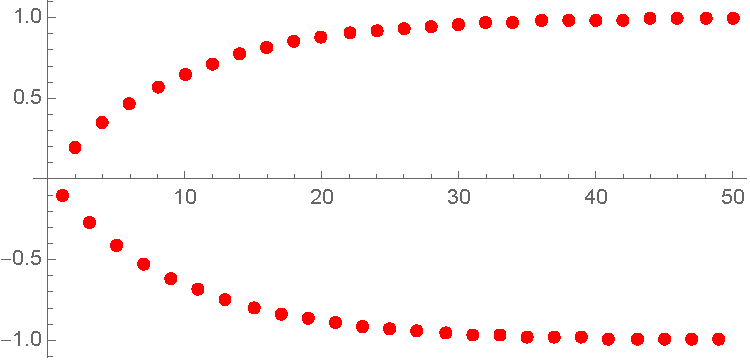
\includegraphics[width=0.5\textwidth]{./Images/Ch01/an109.pdf}
	\caption{一个不收敛的数列:$\{(-1)^n-(0.9)^n\}$}
	\label{fig:an-diverse}
\end{figure}

\bs
{\bf 2. 有界性}
\begin{thx}
	{\bf 定理:}数列$\{a_n\}$若收敛,则{\it $\{a_n\}$有界},
	即:存在$M>0$,对任意$n\in\mathbb{Z}_+$,恒有$|a_n|\leq M$。	
\end{thx}

提示:利用$\e$的特定取值“控制”$n>N$的部分,而在$N$之前的
有限多个数构成的集合自然是有界的。

解:记$\limn a_n=a$。由极限的定义,对{\b$\e=1$},存在$N\in\mathbb{Z}_+$,
对任意$n>N$,有
$$|a_n-a|<\e=1\quad\Rightarrow\quad |a_n|<|a|+1.$$
记$M=\max\{|a|+1,|a_1|,|a_2|,\ldots,|a_{[N]+1}|\}$,则对
任意$n\in\mathbb{Z}_+$,均有
$$|a_n|\leq M,$$
即证。\fin

\begin{figure}[h]
	\centering
	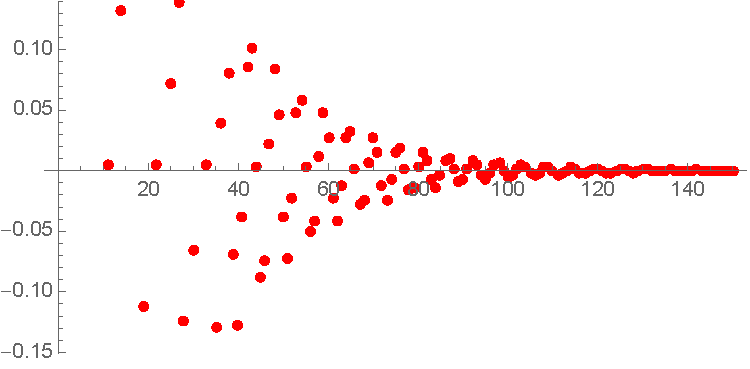
\includegraphics[width=0.5\textwidth]{./Images/Ch01/095nsin2n.pdf}
	\caption{一个收敛的数列:$\{(-0.95)^n\sin2n\}$}
	\label{fig:an-converge}
\end{figure}

该性质的等价命题(逆否命题)常被用来证明数列发散:
{\bf 如果某数列无界,则必发散。}

\begin{shaded}
	\egz 讨论$\{\sqrt[n]{n!}\}$的敛散性。
	\pss{\centering
	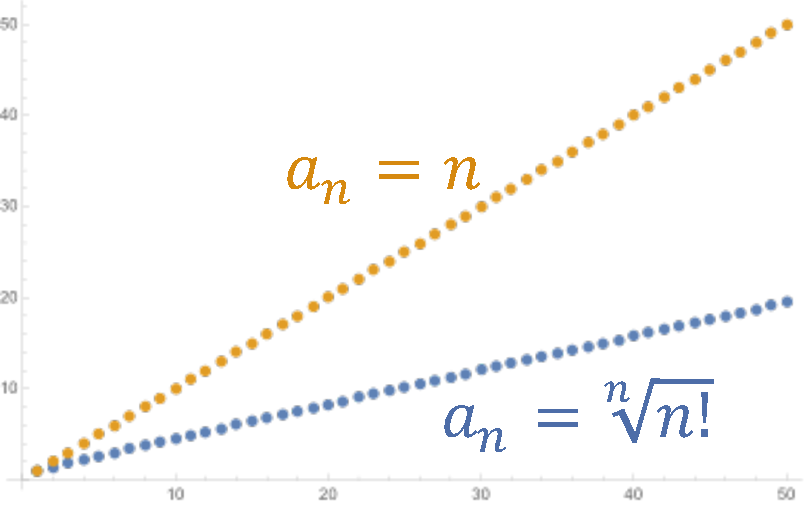
\includegraphics[width=0.9\marginparwidth]{./Images/Ch01/nnnf.pdf}}

	提示:对任意$M>0$,当$n$充分大时,总有$n!>M^n$,
	故$\{\sqrt[n]{n!}\}$无界,从而发散。

	证:对任意$M>0$,令$N=[2M]+1$,则当$n>N$时,总有$n>2M$。此时
	$$\df{n!}{M^n}=\df{N!}{M^N}\cdot\df{N+1}{M}
	\cdot\df{N+2}{M}\ldots\df{n}{M}>\df{N!}{M^N}\cdot2^{n-N}.$$
	注意到$\df{N!}{M^N}$为有限值,而$2^{n-N}$随着$n$的增大趋于正无穷,
	故当$n$充分大时,必有
	$$\df{n!}{M^n}=\df{N!}{M^N}\cdot2^{n-N}>1,$$
	从而$\sqrt[n]{n!}>M$,也即$\{\sqrt[n]{n!}\}$无界,故发散。\fin
\end{shaded}

\bs
{\bf 3. 保号性}
\begin{thx}
	{\bf 定理:}设$\lim\limits_{n\to\infty}a_n=a>0$,则存在$N$,
	对任意$n>N$,$a_n>0$	
\end{thx}

证:由$\lim\limits_{n\to\infty}a_n=a>0$,对$\e=a/2$,存在
$N$,对任意$n>N$,
$$|a_n-a|<\e=a/2\quad\Rightarrow\quad \df32a>a_n>a/2>0,$$
即证。\fin
		
保号性有几种不同的表达形式:
\begin{thx}
	\begin{enumerate}[\bf 推论1:]
% 	  \setlength{\itemindent}{1cm}
	  \item 对任意$n\in\mathbb{N}$,$a_n\geq
	  0$, $\lim\limits_{n\to\infty}a_n=a$, 则$a\geq 0$
	  \item 设$\lim\limits_{n\to\infty}a_n=a\ne
	  0$, 则$\exists N$,当$n>N$时,$|a_n|>|a|/2$
	  \item  设$\lim\limits_{n\to\infty}a_n=a$, 且最多有有限
	  个$a_n$小于零, 则$a\geq 0$
	\end{enumerate}	
\end{thx}

保号性的实质,是{\it 极限运算保持不等号的方向
\ps{但严格大(小)于可能变成大(小)于等于}不变},
若已知$\limn a_n=a,\limn b_n=b$,则
$$a_n\geq b_n\,(n\in\mathbb{Z}_+)\quad\Rightarrow
\quad\limn a_n\geq\limn b_n.$$

\bs
{\bf 4. 数列与子数列的敛散性的关系}

{\bf 子数列}是指从原数列中“取出”无穷多个数所构成的新数列,
新数列中每个数出现的先后次序与原数列中相一致。子数列通常记为
$\{a_{n_k}\}$,其中$\{n_k\}$必须是一个严格单调递增的正整数列。
显然,对任意$k\in\mathbb{Z}_+$,$n_k\geq k$。

例如,数列$\{a_n\}$的{\it 偶子列}和{\it 奇子列}可分别
记为$\{a_{2k}\}$、$\{a_{2k-1}\}$,有时也直接写为
$\{a_{2n}\}$、$\{a_{2n-1}\}$。

在子数列中,$k$是真正的自变量,$n_k$是随$k$变化的,或者说,
如果将子数列看成是两个整序函数的复合函数,
则$n_k$可以视为该复合函数的一个中间变量。因此,相应地,其
极限的定义如下:

{\bf 子数列$\{a_{n_k}\}$以$a$为极限},
是指:对任意$\e>0$,存在$K\in\mathbb{Z}_+$,使对任意$k>K$,总有
$$|a_{n_l}-a|<\e.$$
记为
$$\lim\limits_{k\to\infty}a_{n_k}=a,\quad 
\mbox{或}\quad a_{n_k}\to a\;{(k\to\infty)}.$$

\begin{thx}
	{\bf 定理(收敛数列与其子数列的关系):}数列$\{a_n\}$收敛,
	当且仅当它的所有子列均收敛到相同的极限。
\end{thx}

\begin{figure}[h]
	\centering
	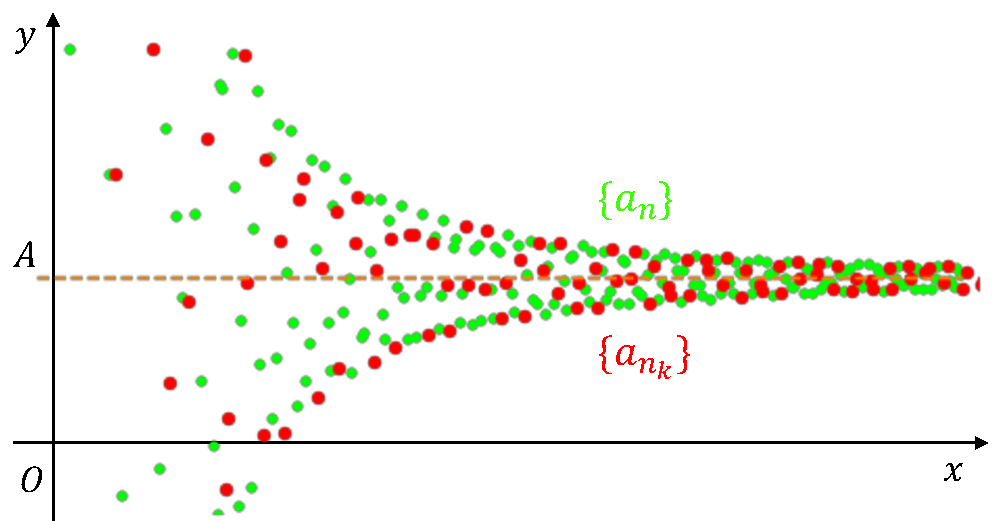
\includegraphics[width=0.5\textwidth]{./Images/Ch01/anank.pdf}
	\caption{若$\{a_n\}$收敛,则它的任意子列$\{a_{n_k}\}$一定
	和它有着完全相同的收敛性质,\\
	形象地说,就是要”随大流“}
	\label{fig:anank}
\end{figure}

证:充分性是显然的,因为$\{a_n\}$可以看成是自身的一个子列。

下面证明必要性。设$\limn a_n=a$,则对任意$\e>0$,存在$N\in\mathbb{Z}_+$,
使对任意$n>N$,有$|a_n-a|<\e$。

设$\{a_{n_k}\}$为$\{a_n\}$的任一子列。令$K=N$,则由$\{n_k\}$严格单调递增,
可知对任意$k>K$,都有$n_k>n_K\geq K=N$,从而 
$$|a_{n_k}-a|<\e.$$
也即$\lim\limits_{k\to\infty}a_{n_k}=a$。因为$\{a_{n_k}\}$是任意的,即证。
\fin
	
\bs
该定理的一个明显用途,是判定一些数列的发散。也即,{\bf 若某个数列存在
发散的子数列,或者存在两个收敛到不同极限的子数列,则该数列必发散。}

\egz 证明数列$\{(-1)^n\}$发散。

证:取该数列的偶子列和奇子列,分别为$\{a_{2k}\}$和$\{a_{2k-1}\}$。显然,
对任意$k\in\mathbb{Z}_+$,都有
$$a_{2k}\equiv 1,\quad a_{2k-1}\equiv -1,$$
因此
$$\lim\limits_{k\to\infty}a_{2k}=1,\quad
\lim\limits_{k\to\infty}a_{2k-1}=-1.$$
由二者极限不相等可知原级数发散,即证。\fin

这种方法证明发散,比前面使用数列收敛的反面定义或反证法
来证明要更加简洁,也更加直观。

\bs
\egz \ps{KD教材2.2.2节-例4}
证明数列$\left\{n^{(-1)^n}\right\}$发散。

提示:原数列存在发散子列$\left\{(2n)^{(-1)^{2n}}\right\}=\{2n\}$。

\bs
{\bf 思考:} 证明$\left\{\left(1+\df1{\sqrt n}\right)
\sin\df{\pi\sqrt n}2\right\}$
发散。

\ifhint
提示:取$n_k=k^2$。 
\fi

\begin{shaded}
	证明数列发散往往比证明其收敛更困难,因为要证明所有的数都不是其极限。
	因此,在证明方法上,也更加多样。下面的例子请自行阅读,我们不作要求。

	\egz 证明:$\{\sin n\}$发散。

	\pss{\centering
	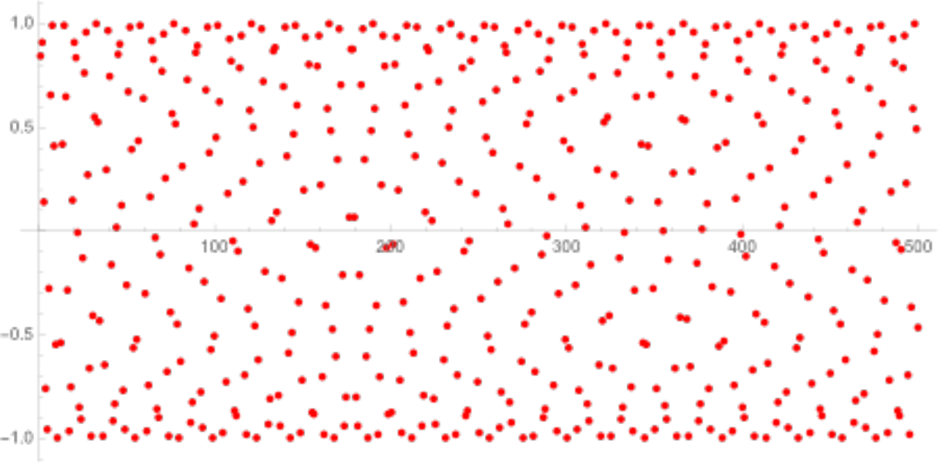
\includegraphics[width=0.9\marginparwidth]
	{./images/ch01/sin-n.pdf}\\
	数列$\{\sin n\}$
	}
	
	证法一:反证法。设有$\limn\sin n=a$,则
	$$\limn[\sin(n+2)-\sin n]=0.$$
	进而由
	$$\sin(n+2)-\sin n=2\sin 1\cos(n+1),$$
	可得$\limn\cos(n+1)=0$。又
	$$\cos(n+1)=\cos n\cos 1-\sin n\sin 1,$$
	可得$\limn\sin n=0$。如此就有
	$$\limn\sin n=\limn\cos n=0,$$
	显然与$\sin^2n+\cos^2n=1$矛盾。\fin
	
	证法二:注意到当$x\in[2k\pi+\pi/4,2k\pi+3\pi/4]\,
	(k\in\mathbb{N})$时,总有
	$$\sin x>\sqrt2/2.$$
	由于此类区间的长度均超过$1$,故其中必包含至少一个自然数。
	于是对每个$k\in\mathbb{N}$,
	可取自然数$n^{(1)}_k\in[2k\pi+\pi/4,2k\pi+3\pi/4]$,
	显然$\{\sin{n^{(1)}_k}\}$构成了$\{\sin
	n\}$的一个子列。
	
	若$\{\sin n\}$收敛,则$\{\sin{n^{(1)}_k}\}$也收敛,且与之极限相同。由极限的保号性,
	可知$\{\sin{n^{(1)}_k}\}$的极限不小于$\sqrt2/2$,从而$\{\sin
	n\}$的极限应大于等于$\sqrt2/2$。
	
	同理,利用区间$[2k\pi+5\pi/4,2k\pi+7\pi/4]\,(k\in\mathbb{N})$,
	可构造$\{\sin n\}$的另一个子列 
	$\{\sin{n^{(2)}_k}\}$。若$\{\sin n\}$收敛,同样利用保号性可证明其极限应小于等于$-\sqrt2/2$。
	
	以上两方面的结论矛盾,故假设错误,即证。\fin
\end{shaded}

该性质类似的一个结论如下:
\begin{thx}
	{\bf 拉链定理}:若某个数列的奇子列和偶子列收敛到相同的极限,
	则该数列收敛。
\end{thx}

请自行尝试证明该定理。注意,这个定理并不是子数列性质的简单推论。
此外,还请想一想,这个定理可以进一步推广吗?

事实上,拉链定理有更一般形式的推广:如果选择的多个子列按顺序
合并起来能够完全覆盖原数列,
或最多不能覆盖原数列中有限多个数,且这些子列均收敛于相同的极限,
则原数列收敛。
例如:{\it 若子数列$\{a_{3n}\},\{a_{3n-1}\},\{a_{3n-2}\}$
都收敛于$a$,
则$\{a_{n}\}$收敛于$a$。}

\begin{shaded}
{\bf Cauchy命题}

以下结论不容易证明,但结论很直观,了解即可
\ps{证明参见菲赫金哥尔茨《微积分学教程》第一卷第一章第2节}:
\begin{tcolorbox}
	{\bf Cauchy命题}:若$\limn a_n=a$,
	则$\limn\df{a_1+a_2+\ldots+a_n}n=a$。
\end{tcolorbox}

这个结论也称为Cauchy{\it 极限},有着非常重要的应用,例如,今后我们会学习
下面的极限$\limn\sqrt[n]a=1,\,(a>0)$,于是立即可以得到
$$\limn\df1n(a+\sqrt[2]a+\sqrt[3]a+\ldots+\sqrt[n]a)=1.$$

\bs
此外,我们今后还会学习到极限运算和初等函数运算可以交换次序,
进而可以证明如下的定理:

\begin{tcolorbox}
	{\bf 定理:}设$a_n$均大于零,且$\limn\df{a_{n+1}}{a_n}=q$,则
	$\limn\sqrt[n]{a_n}=q$。	
\end{tcolorbox}

证:记$b_1=a_1$,$b_n=\df{a_n}{a_{n-1}}\;(n>1)$,则
$$a_n=b_n\cdot b_{n-1}\cdots b_1,$$
进而
$$\ln a_n=\ln b_n+\ln b_{n-1}+\ldots+\ln b_1,$$
已知$\limn b_n=q$,根据初等函数的性质,可得$\limn\ln b_n=\ln q$,
于是由Cauchy极限,
$$\limn\ln \sqrt[n]{a_n}=\limn\df1n\ln a_n=\limn\df1n\left(
\ln b_n+\ln b_{n-1}+\ldots+\ln b_1\right)=\ln q,$$
进而可得$\limn\sqrt[n]{a_n}=q$。\fin 

\bs
有了这个定理,我们很容易得到下面的结论:
\begin{tcolorbox}
	{\bf 定理:}设$a_n$均大于零,且$\limn a_n=a$,则
	$\limn\sqrt[n]{a_1a_2\ldots a_n}=a.$
\end{tcolorbox}
\end{shaded}

\begin{ext}
	{\centering\bf 习题1-2}
	
	\begin{enumerate}  
	  \item 用定义证明如下极限:
	  \begin{enumerate}[(1)]
	    \item $\limn\df{\sqrt{n^2+a^2}}n=1$;
	    \item $\limn0.\underbrace{999\ldots9}_{n\mbox{\footnotesize 个}}=1$;
	    \item $\limn(\sqrt[3]{n+1}-\sqrt[3]n)=0$;
	    \item $\limn\df{n^2-n-1}{2n^2+2n-4}=\df12$。
	  \end{enumerate}
	  \item 设数列$\{a_n\}$有界,$\limn b_n=0$,证明:$\limn a_nb_n=0$。
	  \item 设$\limn a_n=a\ne 0$,证明:存在$N\in\mathbb{Z}^+$,对任意
	  $n>N$,有$|a_n|>|a|/2$。
	\end{enumerate}
\end{ext}

\section{函数的极限}

\subsection{函数极限的定义}

函数极限是我们后续定义导数、积分的概念的基础。从形式上看,
可以将它视为数列极限的推广,
但从直观意义上看,二者存在很大的不同。

不同于数列极限中自变量$n$只有趋于$\infty$(事实上是趋于$+\infty$)
一种趋势,函数中的变量$x$可能的变化趋势有六种,通常分为两大类:
\begin{itemize}
  \setlength{\itemindent}{1cm}
  \item {\it 自变量$x$趋于无穷}
  \pss{$x\to x_0^+$表示从$x$从大于$x_0$的部分趋近$x_0$,
  一般也称为从正向趋于$x_0$;类似地,$x\to x_0^-$称为从负向趋于
  $x_0$}
  $$x\to\infty,\quad x\to+\infty,\quad x\to-\infty$$
  \item {\it 自变量趋于$x$有限值$x_0$}
  $$x\to x_0,\quad x\to x_0^+,\quad x\to x_0^-$$
\end{itemize}

\bs
{\bf 思考:} $\limn f(n)=A\Leftrightarrow\limx{+\infty}f(x)=A$成立吗?

\ifhint
答:显然,$\limx{+\infty}f(x)=A$可以推出$\limn f(n)=A$,但反之不然,
\ps{事实上,$f(n)$的值域是$f(x)$值域的子集}

例如:$y=\sin\pi x$当$x\to+\infty$时不收敛,但$\limn\sin n\pi=0$。
\fi

\bs
{\bf 1.\;$x$趋于无穷时的函数极限}

参考数列极限的定义,我们可以给出函数当$x$趋于无穷时的极限的定义,这里
我们使用了较简略的写法
\ps{$x\to\infty$表示同时趋向正负无穷,其实质是远离任何一个
固定的点,只有当趋于正负无穷的极限相同时该极限才有意义}:
\begin{thx}
	\begin{enumerate}%[(1)]
	  \item $\limx{+\infty}f(x)=A\quad\Leftrightarrow\quad
	  \forall \e>0,\exists X>0,\forall x>X,|f(x)-A|<\e$
	  \item $\limx{-\infty}f(x)=A\quad\Leftrightarrow\quad
	  \forall \e>0,\exists X<0,\forall x<X,|f(x)-A|<\e$
	  \item $\limx{\infty}f(x)=A\quad\Leftrightarrow\quad
	  \forall \e>0,\exists X>0,\forall |x|>X,|f(x)-A|<\e$
	\end{enumerate}
\end{thx}

显然,这三个极限定义的不同之处主要体现在如何表示$x$的范围方面。例如:
若考虑$x\to+\infty$时的极限,则要说明当$x$充分大(充分靠近$+\infty$)
时,可以使$|f(x)-A|<\e$成立。这里的充分大就可以表示为“{\it 存在
$X$,对任意的$x>X$}”。类似地,,若考虑$x\to\infty$时的极限,则要说明
当$x$充分靠近$\pm\infty$时,可以使$|f(x)-A|<\e$成立。而所谓的
“{\kaishu 充分靠近$\pm\infty$}”{\kaishu 也即"$|x|$充分大}",
因此可以表示为"存在$X$,对任意$|x|>X$"。

\bs
直观上看,若函数当$x$趋于无穷时的极限存在,则意味着其图像存在
{\bf 水平渐近线},例如:反正切函数(参见图\ref{subfig:arctan})
满足
\begin{itemize}
	\item $\limx{+\infty}\arctan x=\frac{\pi}{2}$,故
	当$x\to+\infty$时,$y=\arctan x$有水平渐近线$y=\frac{\pi}{2}$;
	\item $\limx{-\infty}\arctan x=-\frac{\pi}{2}$,故
	当$x\to-\infty$时,$y=\arctan x$有水平渐近线$y=-\frac{\pi}{2}$;
	\item 因为$\limx{+\infty}\arctan x\ne\limx{-\infty}\arctan x$,
	故极限$\limx{\infty}\arctan x$不存在。
\end{itemize}

\begin{figure}[h]
	\centering
	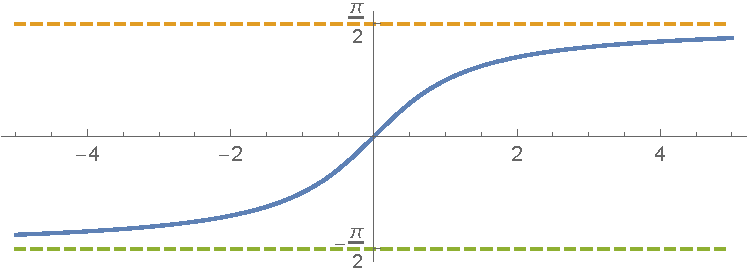
\includegraphics[width=0.5\textwidth]{./Images/Ch01/arcTanAsy.pdf}
	\caption{$\arctan x$和它的两条水平渐近线}
	\label{fig:arctanAsy}
\end{figure}
	
\bs

\egz 证明$\limx{+\infty}\df1{\sqrt x}=0$.

证:对任意$\e>0$,取$X=\df1{\e^2}$,则对任意的$x>X$,都有
$$\left|\df1{\sqrt x}-0\right|=\df1{\sqrt x}<\df1{1/\e}=\e,$$
由函数极限的定义,即证。\fin

\bs

{\bf 2.\;$x$趋于有限值时的函数极限}
\pss{$U_0^+(x_0,\delta)=(x_0,x_0+\delta)$,也即$x_0$
	  的右半$\delta$邻域;同理,$U_0^-(x_0,\delta)$表示
	  $x_0$的左半$\delta$邻域}
\begin{thx}
	\begin{enumerate}%[(1)]
	  \item $\limx{x_0}f(x)=A\quad\Leftrightarrow\quad
	  \forall \e>0,\exists\delta>0,\forall
	  x\in U_0(x_0,\delta),|f(x)-A|<\e.$
	  \item $\limx{x_0^+}f(x)=A\quad\Leftrightarrow\quad
	  \forall \e>0,\exists\delta>0,\forall x\in
	  U_0^+(x_0,\delta),|f(x)-A|<\e.$
	  \item $\limx{x_0^-}f(x)=A\quad\Leftrightarrow\quad
	  \forall \e>0,\exists\delta>0,\forall
	  x\in U_0^-(x_0,\delta),|f(x)-A|<\e.$
	\end{enumerate}
\end{thx}

无论是$x$趋于无穷时的极限还是$x$趋于有限值时的极限,定义的逻辑结构都是
一致的,唯一的不同就在于对$x$变化趋势的表述方法(有限领域和无穷领域的差别)。
抽象地说,以上的六个极限定义都是陈述了如下一个事实:{\kaishu 
$\limx{\Delta}f(x)=A$,也即:随着$x$越来越靠近$\Delta$
($\Delta$代表$x_0,x_0^+,x_0^-,\infty,+\infty$,$-\infty$之一),
$f(x)$的值越来越靠近$A$};或者说,{\it 要使$f(x)$充分
靠近$A$,只需$x$充分靠近$\Delta$}。这与我们对数列极限的定义是完全一致的。

\bs

{\bf 课堂练习:} \ps{KD教材习题3.1-1}
根据图形(图\ref{fig:limxexist})判断极限的存在性,若存在给出其值
\begin{figure}[h]
	\centering
	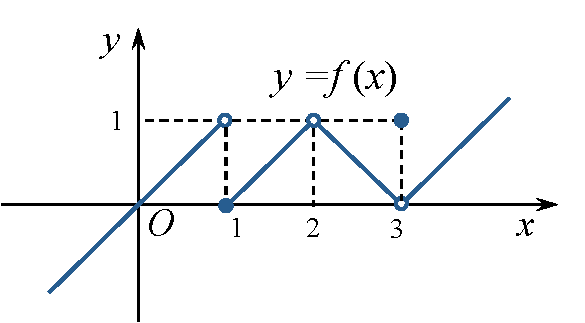
\includegraphics[width=0.4\textwidth]{./Images/Ch01/limxf.pdf}
	\caption{$\limx{1}f(x)$\underline{不存在}
	\quad $\limx{2}f(x)$\underline{$=1$}
	\quad $\limx{1}f(x)$\underline{$=0$}}
	\label{fig:limxexist}
\end{figure}

\bs
{\bf 讨论:}
\begin{enumerate}
  \setlength{\itemindent}{1cm}
  \item 为什么在定义中要求$0<|x-x_0|<\delta$,而不是$|x-x_0|<\delta$?
   
   \quad 答:因为极限表示的$x\to x_0$时的过程中函数值的变化趋势,
   与函数在$x_0$处的取值无关!例如:令$f(x)=|\mathrm{sgn}(x)|$,
   则$\limx{0}f(x)=1$,但是$f(0)=0$。
  \item 符号$f(x_0+0),f(x_0-0)$与$f(x_0)$是何关系?
  
  \quad 答:前两者分别表示左、右极限
  \ps{类似地,$x$趋向无穷时的极限也可以记为:$f(\infty)$,$f(+\infty)$
  和$f(-\infty)$}
  ,最后一个是函数值,三者相互无关。
  例如:令$f(x)=\mathrm{sgn}(x)$,则$f(x_0+0)=1$,$f(x_0-0)=-1$,
  $f(0)=0$。
\end{enumerate}

\bs
\egz 证明:$\limx{x_0}\sin x=\sin x_0$。

证:对任意$\e>0$,令$\delta=\e$
\ps{寻找合适的$\delta$是证明的关键},则当$0<|x-x_0|<\delta$时,有
$$|\sin x-\sin x_0|=2\left|\cos\df{x+x_0}2\right|
\left|\sin\df{x-x_0}2\right|\leq|x-x_0|<\delta=\e,$$
由函数极限定义,即证。\fin

\bs

\egz 证明:$\limx{1}x^2=1$。

证:对任意$\e>0$,令$\delta=\min\left\{\df12,\e\right\}$,
\ps{令$\delta\leq\df12$,作用在于使得$|x+1|$有界}
则当$0<|x-1|<\delta$时,有
$$|x^2-1|=|(x+1)(x-1)|<\df32\cdot\delta<\df32\e,$$
由函数极限定义,即证。\fin

注:和数列极限类似,在函数极限的定义中,最后不等式右端
的$\e$可以改写为$C\e$,
其中$C>0$为常数,所得命题与原定义等价。

\bs

\egz 设$\limx{x_0}f(x)=A$,用定义证明:$\limx{x_0}[f(x)]^3=A^3$

证:对任意$\e>0$,由$\limx{x_0}f(x)=A$,存在$\delta>0$,对任意
$0<|x-x_0|<\delta$,有
$$|f(x)-A|<\e.$$
不妨设$\e<1$,由上式可知$0<|x-x_0|<\delta$时,有$|f(x)|<|A|+1$。

综上,记$C=(|A|+1)^2+(|A|+1)|A|+A^2$,则当$0<|x-x_0|<\delta$时,总有
\begin{align}
	|f^3(x)-A^3|&=|f(x)-A||f^2(x)+f(x)A+A^2|\notag\\
	&\leq |f(x)-A|[|f^2(x)|+|f(x)||A|+A^2]\notag\\
	&<\e[(|A|+1)^2+(|A|+1)|A|+A^2]=C\e\notag,
\end{align}
有极限的定义,即证。\fin

\begin{shaded}
	\begin{tcolorbox}
		{\bf 函数极限的反面说法}
		\begin{itemize}
		  \item {\it $\limx{x_0}f(x)\ne A$}$\Leftrightarrow$ 
		    $\exists\e_0>0,\forall\delta>0, \exists x^*\in
		    U_0(x_0,\delta),|f(x^*)-A|\geq\e_0$ 
		  \item {\it $\limx{x_0}f(x)\ne A$不存在}$\Leftrightarrow$
			$\forall A\in\mathbb{R},\exists\e_0>0,\forall\delta>0, \exists x^*\in
		    U_0(x_0,\delta),|f(x^*)-A|\geq\e_0$ 
		\end{itemize}
	\end{tcolorbox}

	\egz 证明:Dirichlet函数在任意点处无极限。
	
	证:任取$x_0,A\in\mathbb{R}$,不妨设$A\ne 0$($A\ne 1$的情况同理可证)。
	
	令$\e_0=\df{|A|}2$,对任意$\delta>0$,由无理数的稠密性,总可以在
	$U_0(x_0,\delta)$内取得某个无理数$x^*$,从而$D(x^*)=0$,于是
	$$|D(x^*)-A|=|A|>\e_0,$$
	由上述的定义,可知当$x\to x_0$时$D(x)$无极限,又由$x_0$的任意性,可知
	$D(x)$处处无极限。\fin

	\bs
	
	{\bf 思考:}证明:函数$f(x)=xD(x)$只在$x=0$处收敛。

	注意,证明应该包括两个部分,一是证明$xD(x)$在$x=0$处收敛,二是证明
	$xD(x)$在任意$x\ne 0$处发散。
\end{shaded}

\subsection{函数极限的基本性质}

参考数列极限的性质,可以类似地证明函数极限的下列性质。

为了指出这些性质与数列极限的类似性质在表述上的差异,
这里分别以$x\to+\infty$和$x\to x_0$
两种情形为例叙述一遍(证明略):

{\kaishu 情形1.} $x\to+\infty$时函数极限的性质:

设$x\to+\infty$时函数$f(x)$收敛,则:
\begin{itemize}
	\setlength{\itemindent}{1cm}
	\item {\kaishu 唯一性:}$\limx{+\infty}f(x)$唯一确定。
	\item {\kaishu 有界性:}存在$M$和$X$,对任意$x>X$有,
	$|f(x)|\leq M$。
	\item {\kaishu 保号性:}
	\begin{enumerate}[(1)]
		\setlength{\itemindent}{1cm}
		\item 若$\limx{+\infty}f(x)=A>0$,则
		存在$X$,对任意$x>X$,$f(x)>0$.
		\item 若存在$X$,对任意$x>X$,总有$f(x)>0$,
		则$\limx{+\infty}f(x)\geq 0$.
	\end{enumerate}
\end{itemize}

关于保号性,可以参考数列极限的保号性写出若干推论,这里不再赘述。

{\kaishu 情形2.}$x\to x_0$时函数极限的性质:

设$x\to x_0$时函数$f(x)$收敛,则:
\begin{itemize}
	\setlength{\itemindent}{1cm}
	\item {\kaishu 唯一性:}$\limx{x_0}f(x)$唯一确定。
	\item {\kaishu 有界性:}存在$M$和$\delta>0$,对任意
	$x\in U_0(x_0,\delta)$有,$|f(x)|\leq M$。
	\item {\kaishu 保号性:}
	\begin{enumerate}[(1)]
		\setlength{\itemindent}{1cm}
		\item 若$\limx{+\infty}f(x)=A>0$,则
		存在$\delta>0$,对任意$x\in U_0(x_0,\delta)$,$f(x)>0$.
		\item 若存在$\delta>0$,对任意$x\in U_0(x_0,\delta)$,
		总有$f(x)>0$,则$\limx{+\infty}f(x)\geq 0$.
	\end{enumerate}
\end{itemize}

注意到以上两种情形下函数极限的性质有很大相似性,对于更一般的
极限的基本性质,我们可以总结如下:

\begin{thx}
	{\bf $x\to\Delta$时函数极限的性质:}

	设$x\to\Delta$时函数$f(x)$收敛,则:
	
	{\bf 唯一性:}$\limx{\Delta}f(x)$唯一确定。
	
	{\bf 有界性:}存在$M$,使当$x$充分靠近$\Delta$时,
	$|f(x)|\leq M$。
	
	{\bf 保号性:}
	\begin{enumerate}[(1)]
		\setlength{\itemindent}{1cm}
		\item 若$\limx{\Delta}f(x)=A>0$,则
		当$x$充分靠近$\Delta$时,$f(x)>0$.
		\item 若当$x$充分靠近$\Delta$时,
		总有$f(x)>0$,则$\limx{\Delta}f(x)\geq 0$.
	\end{enumerate}
\end{thx}

以上的$\Delta$可以任意代表$\infty,+\infty,-\infty,x_0,x_0^+,
x_0^-$之一。而所谓{\kaishu $x$充分靠近$\Delta$}则需要根据$\Delta$
的不同有不同的表述。

函数极限有界性和数列极限有界性的叙述存在的差异:
数列收敛则数列整体有界(数列极限中的数列整体都有界,
是由数列自身的“稀疏”特性所决定的),
函数收敛只能说明在趋近的过程中(或者充分靠近目标时)有界!

例如:极限$\limx{+\infty}\df1x=0$,但$\df1x$在定义域上无界;
类似地,$\limx{1}x=1$,但$x$显然也是无界的。

\bs
\pss{Henie(1821-1881),德国数学大师Weierstrass的学生。
	1872年证明:有界闭区间上的连续函数必是一致连续的。
	也即,如果把函数的定义限定在闭区间上,
	连续和一致连续的差别将随之消失。} 
\begin{thx}
	{\bf 函数极限与数列极限的关系}({\kaishu Henie定理}):
	已知$\limx{x_0}f(x)=A$,若数列$\{x_n\}$取值在$f(x)$的定义域内,
	且满足:$x_n\to x_0(n\to$ $\infty)$,$x_n\ne x_0\;
	(n\in\mathbb{Z}_+)$,
	则必有$\limn f(x_n)=A$。
\end{thx}

\begin{figure}[h]
	\centering
	\begin{subfigure}[t]{0.45\textwidth}
		\centering
		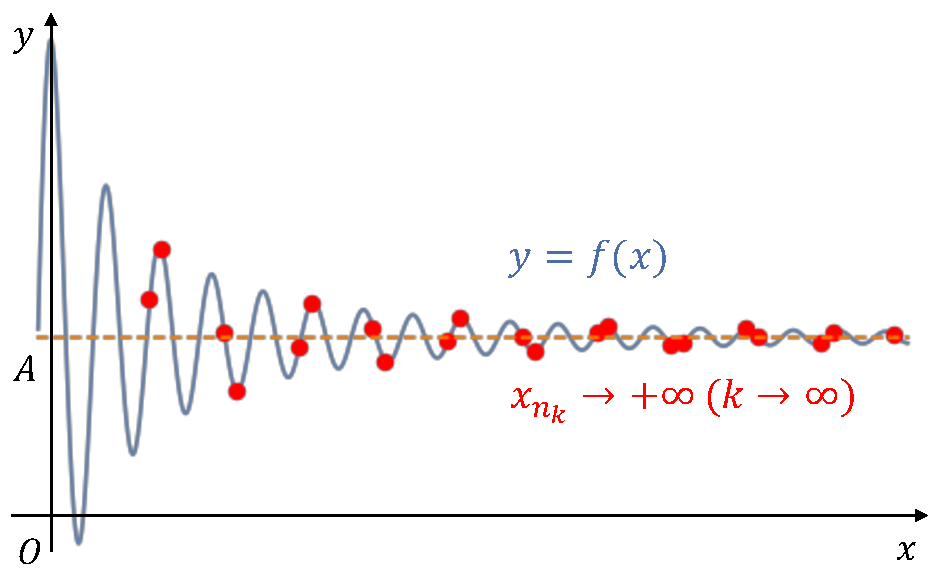
\includegraphics[width=\textwidth]{./Images/Ch01/HenieXnInf.pdf}
		\subcaption{若$\{x_n\}$趋于$+\infty$,则$\limn f(x_n)
		=\limx{+\infty}f(x)=A$}
	\end{subfigure}
	\begin{subfigure}[t]{0.45\textwidth}
		\centering
		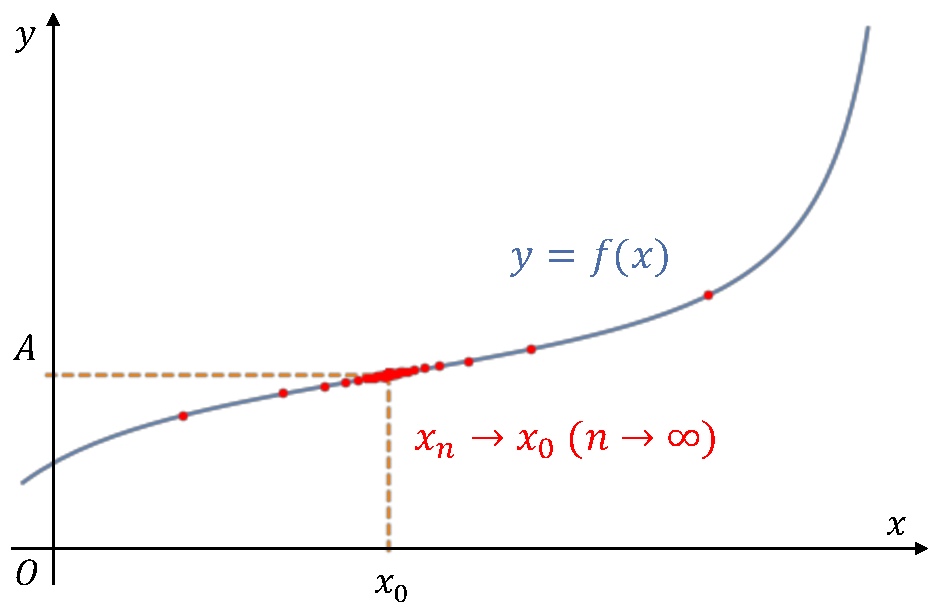
\includegraphics[width=\textwidth]{./Images/Ch01/HenieXnX0.pdf}
		\subcaption{若$\{x_n\}$趋于$x_0$,则$\limn f(x_n)
		=\limx{x_0}f(x)=A$}
	\end{subfigure}
	\caption{Henie定理表达的性质与子数列的收敛性类似}
	\label{fig:Henie}
\end{figure}

证:已知$\limx{x_0}f(x)=A$,故对任意$\e>0$,存在$\delta>0$,
使对任意$x\in U_0(x_0,\delta)$,都有$|f(x)-A|<\e$。

设$\limn x_n=x_0$,则以上的$\delta>0$,存在$N\in\mathbb{Z}_+$,
使对任意$n>N$,都有$|x_n-x_0|<\delta$。从而,当$n>N$时,必有
$$|f(x_n)-A|<\e.$$
即证。\fin

对于$x\to x_0^+$和$x\to x_0^-$的情形,该定理显然也成立。

与上一节子数列有关收敛性质的用途一样,
\pss{由于计算函数极限有类似L'Hospital法则和Taylor公式
这样的工具,相对来说比计算数列极限方法更多样}
Henie定理的用途更多地是证明函数极限不存在。
当然,有时遇到一些不方便计算的数列极限,
也可能将其转化为对应的函数极限来计算。

\bs
\egz 证明:$f(x)=\sin\df 1x$当$x\to 0$时无极限。

证:令\ps{如图\ref{fig:sin1x1-1}}
$$x^{(1)}_n=\df1{n\pi},\quad
x^{(2)}_n=\df1{2n\pi+\frac{\pi}2},\quad n\in\mathbb{Z}_+$$ 
显然,$\limn x^{(1)}_n=\limn x^{(2)}_n=0$,且
$$f(x^{(1)}_n)\equiv0,\quad f(x^{(2)}_n)\equiv1,$$
进而
$$\limn f(x^{(1)}_n)=0\ne1=\limn f(x^{(2)}_n),$$
由Henie定理,即知极限不存在。\fin

\begin{figure}[h]
	\centering
	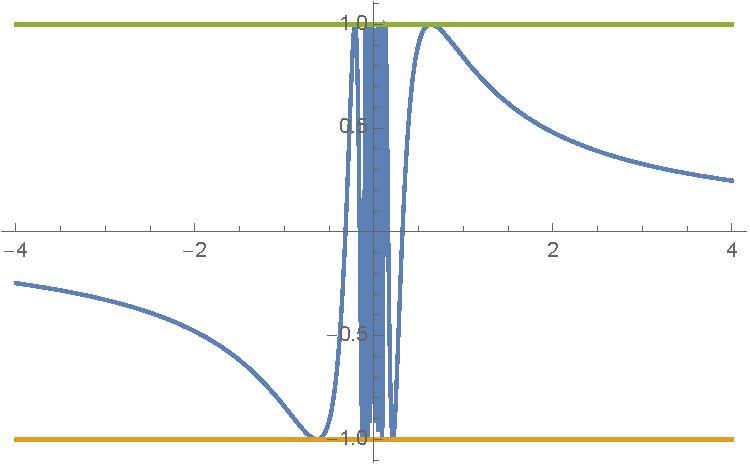
\includegraphics[width=0.5\textwidth]{./Images/Ch01/sin1x.pdf}
	\caption{以上所取的$x^{(1)}_n$和$x^{(2)}_n$分别取自图上绿色和黄色水平线与
	函数$\sin\df1x$的交点,事实上,对于任意的$a\in[-1,1]$(红色水平线),
	都可以取得类似的点列,用于构造证明所需的收敛到不同值得函数值数列,请思考以下如何写
	出其表达式?}
	\label{fig:sin1x1-1}
\end{figure}

\begin{figure}[htbp]
	\centering
	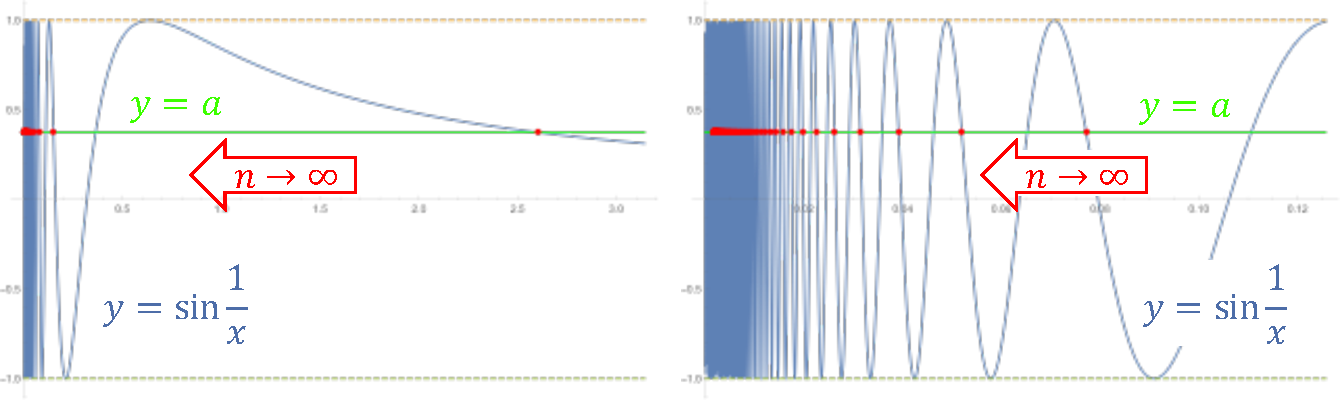
\includegraphics[width=\textwidth]{./Images/Ch01/sin1xa.pdf}
	\caption{$x^{(a)}_n=\df1{2n\pi+\arcsin a},\quad n\in\mathbb{Z}_+$}
	\label{fig:sin1xa}
\end{figure}

\bs
\egz 用Henie定理证明Dirichlet函数在任意点处无极限。
	
证:
对任意$x_0$,定义
$$x_n=[x_0]+x_0\mbox{\it 小数部分的前}n\mbox{\it 位},$$
$$x_n^{(1)}=x_n+\df1n,\quad
x_n^{(2)}=x_n+\df{\sqrt2}n,$$
显然$\{x_n^{(1)}\}$和$\{x_n^{(2)}\}$分别为趋于$x_0$的有理和无理数列,而
$$\limn D(x_n^{(1)})=1\ne0=\limn D(x_n^{(2)}),$$
从而由Hiene定理,即证。\fin

\bs
\begin{ext}
	{\centering\bf 习题1-3}
	
	\begin{enumerate}  
	  \item 用定义证明如下极限:
	  \begin{enumerate}[(1)]
	    \item $\limx{-2}{x^2}=4$;
	    \item $\limx{+\infty}\df{\sin x}{\sqrt x}=0$;
	    \item $\limx{\infty}\df{x+\sin x}{x+\cos x}=1$.
	  \end{enumerate}
	  \item (选作)证明:$f(x)=xD(x)$仅当$x=0$时极限存在。($D(x)$表示Dirichlet函数)
	\end{enumerate}
\end{ext}

\section{无穷小与无穷大}

无穷小和无穷大是对极限的一种描述方式,接下来的有关性质为
我们后续讨论极限的各种性质,以及进行极限的计算提供了更为
简洁方便的表达方式。

\subsection{无穷小}

以下$\Delta$表示$x_0,x_0^+,x_0^-,\infty,+\infty,-\infty$
中的之一。

\pss{\baa 引入类似$\circ(\cdot)$的符号,是为了运算时的方便,但是必须
	意识到其意义并不是指一个确定的函数,而是说等号左边的函数具有特定的性质,
	或者说,$\circ(\cdot)$应该被理解为一类函数。
	换个角度来说,“$=\circ(\cdot)$”更应该被视为一个整体,
	$f(x)=\circ(1)$表示
	$f(x)$是满足$\limx{\Delta}f(x)=0$的众多函数中的一个。\\
	一般来说,下面的写法总是错误的:
	$$\circ(1)-\circ(1)=0\;(x\to\Delta)$$}
\begin{thx}
	若$\limx{\Delta}f(x)=0$,则称{\bf $f(x)$为$x\to\Delta$时的无穷小},记为
	$$f(x)=\circ(1),\;(x\to\Delta).$$
\end{thx}

注意,谈到无穷小,一定是和某个变化过程相对应的。
无穷小,但不是$x\to 2$时的无穷小。

显然,常值函数$f(x)\equiv 0$是任何过程中的无穷小。

\bs
利用函数极限和无穷小的定义,容易证明:
\begin{thx}
	{\bf 定理:}$\limx{\Delta}f(x)=A\Leftrightarrow f(x)=A+\alpha$,
	其中$\alpha$是$x\to\Delta$时的无穷小。
\end{thx}
该结论也可以简写为:
$$\limx{\Delta}f(x)=A\quad\Leftrightarrow\quad 
f(x)=A+\circ(1),\;(x\to\Delta)$$

\bs
进一步地,由无穷小的定义,不难证明:
\pss{$f(x)$当$x\to\Delta$时有界,是指$f(x)$在$\Delta$
	  的某邻域内有界}
\begin{thx}
	{\bf 无穷小的性质:}
	\begin{enumerate}
	  \item 在同一过程中的{\it 有限多个}无穷小的和也是该过程中的无穷小,也即
	  $$\underbrace{\circ(1)+\circ(1)+\ldots+\circ(1)}
	  _{\mbox{有限多个}}=\circ(1),\;(x\to\Delta)$$
	  \item 在同一过程中的有界函数与无穷小的乘积也是该过程中的无穷小,也即
	  对任意的$M(x)$为$x\to\Delta$时的有界量,
	  $$M(x)\cdot\circ(1)=\circ(1),\;(x\to\Delta)$$
	  \item 在同一过程中的任意多个无穷小的乘积也是该过程中的无穷小,也即
	  $$\underbrace{\circ(1)\cdot\circ(1)\cdots\circ(1)}_{\mbox{任意多个}}=\circ(1),\;(x\to\Delta)$$
	\end{enumerate}
\end{thx}

需要注意的是,{\baa 无穷多个无穷小相加未必还是无穷小,
而可能是任意的结果,或者说要视具体的问题而定。
例如:当$n\to\infty$时
$$\underbrace{\df1n+\df1n+\ldots+\df1n}_{n\mbox{\footnotesize 个}}=1\to1,$$
$$\underbrace{\df1{n^2}+\df1{n^2}+\ldots+\df1{n^2}}
_{n\mbox{\footnotesize 个}}=\df1n\to0,$$
$$\underbrace{\df1n+\df1n+\ldots+\df1n}
_{n^2\mbox{\footnotesize 个}}=n\to+\infty.$$
}

\subsection{无穷大}

无穷大意味着在某个过程中,函数的绝对值会无限增大,
这同时也就意味着其倒数会趋于零。

\begin{thx}
	若$\limx{\Delta}\df1{f(x)}=0$,则称{\bf $f(x)$为$x\to\Delta$时的无穷大}。
\end{thx}

{\bf 讨论:}$x\to\Delta$时的无穷大和在$x\to\Delta$的
过程中无界有何异同?

\ifhint
答:{\bf 无穷大一定是无界量,无界量不一定是无穷大}。
例如:$f(x)=x$和$g(x)=x\sin x$都是$x\to\infty$时
的无界量(即:只要$x$充分远离原点,则函数值可以超过任何事先给定的值),
但前者是该过程中的无穷大,后者不是。\fin
\fi

\begin{figure}[h]
	\centering
	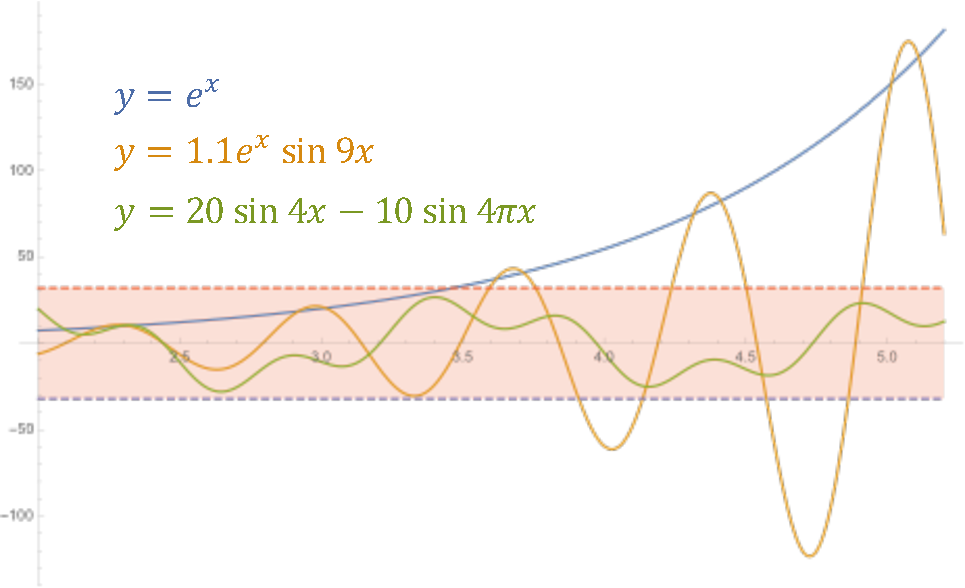
\includegraphics[width=0.6\textwidth]
	{./Images/Ch01/infvsbded.pdf}
	\caption{图中的三个函数分别是$x\to+\infty$
	过程中的无穷大、无界量和有界量}
	\label{fig:infvsbded}
\end{figure}

注意无穷大有正负之分,而无穷小没有。

\bs

除了用无穷小来定义无穷大,无穷大也可以这样来定义:
$f(x)$为$x\to\Delta$时的无穷大,也即:
对于任意$M>0$,当$x$充分靠近$\Delta$时,总有$|f(x)|>M$。
下面就$x\to x_0$的情况给出证明。

\begin{thx}
	{\bf 定理:}$f(x)$为$x\to x_0$时的无穷大,当且仅当:
	对于任意$M>0$,存在$\delta>0$,使对任意$x\in U_0(x_0,\delta)$,
	总有$|f(x)|>M$。
\end{thx}

证:任取$M>0$,令$\e=\df1M$。由无穷大的定义,$\limx{x_0}\df1{f(x)}=0$,故对
此$\e$,存在$\delta>0$,使对任意$x\in U_0(x_0,\delta)$,总有
$$\left|\df1{f(x)}\right|<\e\quad\Rightarrow |f(x)|>\df1{\e}=M.$$
即证。\fin

\bs
$x$趋于有限值时的无穷大对应的是函数曲线的{\bf 铅直渐近线}。
例如:(如图\ref{fig:verAsy})
\begin{itemize}
	\setlength{\itemindent}{1cm}
	\item $\limx{1}(x-1)=0$,故$x=1$是$f(x)=\df1{x-1}$的铅直渐近线;
	\item $\limx{\frac{\pi}{2}^+}\tan x=-\infty$,故$x=\pi/2$
	是$f(x)=\tan x$的铅直渐近线。
\end{itemize}
	
\begin{figure}[h]
	\centering
	\begin{subfigure}[t]{.45\textwidth}
		\centering
		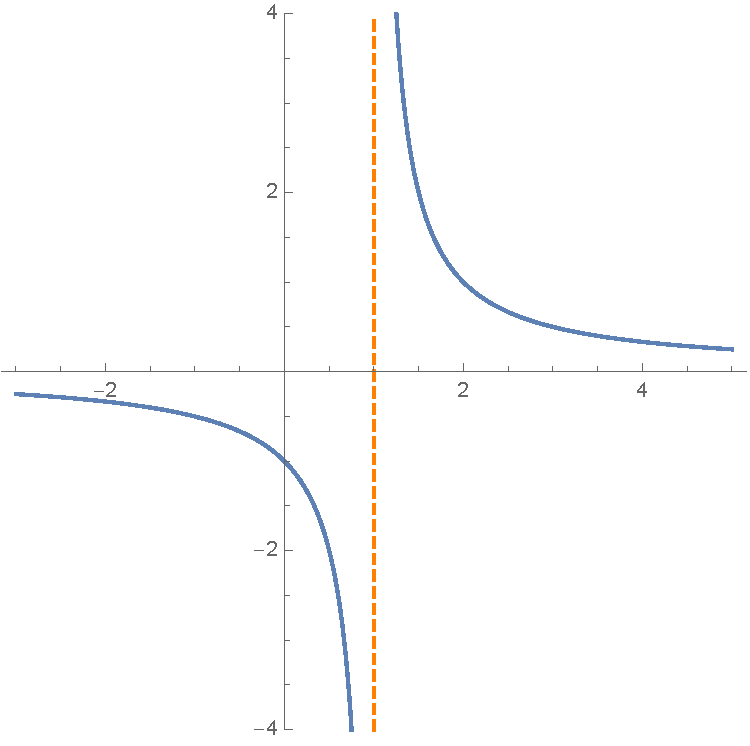
\includegraphics[width=\textwidth]{./Images/Ch01/1x-1Asy.pdf}
		\caption{$y=\df1{x-1}$有铅直渐近线$x=1$}
	\end{subfigure}
	\begin{subfigure}[t]{.45\textwidth}
		\centering
		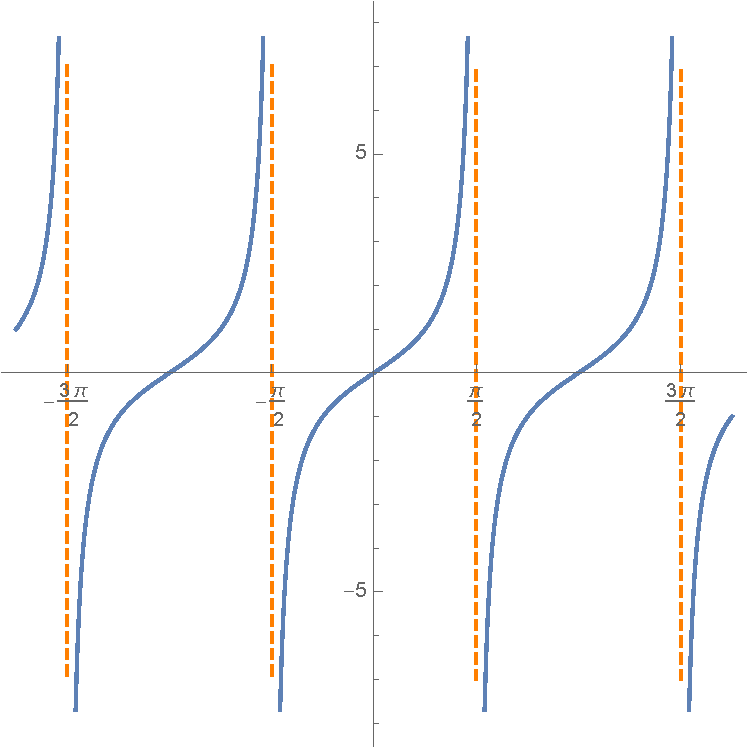
\includegraphics[width=\textwidth]{./Images/Ch01/TanAsy.pdf}
		\caption{$y=\tan x$的铅直渐近线}
	\end{subfigure}
	\caption{铅直渐近线}
	\label{fig:verAsy}
\end{figure}

\bs 
\pss{\centering
	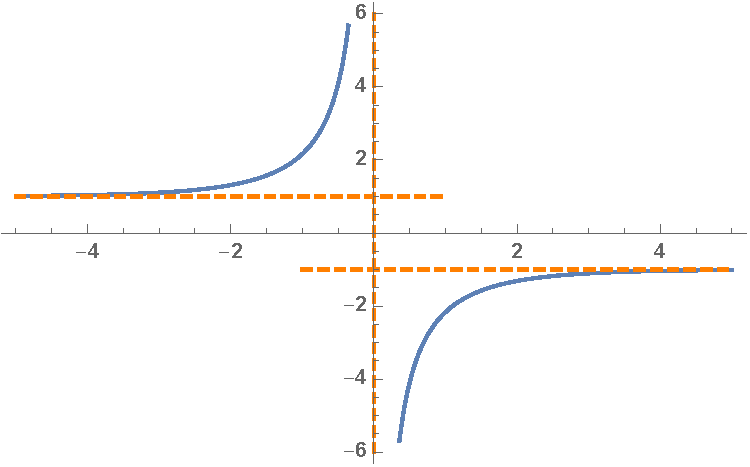
\includegraphics[width=\marginparwidth]{./images/ch01/exOex.pdf}\\
	$y=\df{1+e^x}{1-e^x}$\\
	及其水平和铅直渐近线
}
\egz $f(x)=\df{1+e^x}{1-e^x}$,求曲线$y=f(x)$
的水平和铅直渐近线。

解:因为
$$\limx0\df1{f(x)}=\df{1-\limx0e^x}{1+\limx0e^x}=0,$$
故$f(x)$是$x\to 0$时的无穷大,从而可知$x=0$是$y=f(x)$
的铅直渐近线。

又
$$\limx{+\infty}\df{1+e^x}{1-e^x}
=\limx{+\infty}\df{e^{-x}+1}{e^{-x}-1}
=\df{\limx{+\infty}e^{-x}+1}{\limx{+\infty}e^{-x}-1}
=-1,$$
故$y=-1$是$y=f(x)$的一条水平渐近线。

再由
$$\limx{-\infty}\df{1+e^x}{1-e^x}
=\df{1+\limx{-\infty}e^x}{1-\limx{-\infty}e^x}=1,$$
故$y=1$也是$y=f(x)$的一条水平渐近线。\fin

\bs
\egz 证明多项式函数$f(x)=\sum\limits_{k=1}^{n}a_kx^k$($a_n> 0$)
是$x\to+\infty$时的正无穷大,$x\to-\infty$时的负无穷大。

证:注意到$\limx{+\infty}\df{f(x)}{x^n}=a_n>0$,
由极限的保号性,必存在$X_1>0$,使对任意$x>X_1$,都有
$$\df{f(x)}{x^n}>\df{a_n}2\quad\Rightarrow
\quad f(x)>x^n\df{a_n}2.$$
于是,对任意$M>0$,令$X_2=\sqrt[n]{\frac{2M}{a_n}}$,
则当$|x|>\max\{X_1,X_2\}$时,总有
$$f(x)>x^n\df{a_n}2>M.$$
由此可知$f(x)$是$x\to+\infty$时的正无穷大。

同理可证$f(x)$是$x\to-\infty$时的负无穷大。
\fin

\bs
\egz 设当$x\to x_0$时,$f(x)$不是无穷大,则下列命题中正确的是
(\underline{\quad\quad})
\begin{enumerate}[(A)]
  \setlength{\itemindent}{1cm}
  \item 若$g(x)$是$x\to x_0$时的无穷小,则$f(x)g(x)$必为$x\to x_0$时的无穷小
  \item 若$g(x)$不是$x\to x_0$时的无穷小,则$f(x)g(x)$必不是$x\to x_0$时的无穷小
  \item 若$g(x)$在$x_0$的某邻域内无界,则$f(x)g(x)$必为$x\to x_0$时的无穷大
  \item 若$g(x)$在$x_0$的某邻域内有界,则$f(x)g(x)$必不是$x\to x_0$时的无穷大
\end{enumerate}

\ifhint
提示:不妨以$x\to0$为例,
\begin{enumerate}[(A)]
    \setlength{\itemindent}{1cm}
	\item 反例:$f(x)=\df1x\sin\df1x$,$g(x)=x$;
	\item 反例:$f(x)=0$,$g(x)=1$;
	\item 反例:$f(x)=g(x)=\df1x\sin\df1x$;
	\item 反证法:若$f(x)g(x)$是无穷大,则$\limx0\df1{f(x)g(x)}=0$,
	$g(x)$是有界量,有界量与无穷小的乘积仍为无穷小,
	故$f(x)=\df1{f(x)g(x)}\cdot g(x)$为无穷小,
	从而$f(x)$是无穷大,与已知矛盾!\fin
\end{enumerate}
\fi

\bs
\egz 证明:$f(x)=x\sin x$不是$x\to+\infty$时的无穷大。

证:反证法。假设$f(x)$是$x\to+\infty$时的无穷大,
由无穷大的等价定义,对任意$M>0$,必存在$X$,使对任意
$x>X$总有,$|f(x)|>M$。

然而,若令$x_M=2\pi\left(\left[\frac{X}{2\pi}\right]+1\right)$,
显然$x_M>X$,但
$$f(x_M)=x_M\sin(x_M)=0,$$
从而与假设矛盾,故假设错误。即证。\fin

\bs
\begin{ext}
	{\centering\bf 习题1-4}
	
	\begin{enumerate}  
	  \item 证明:函数$y=\df1x\sin\df1x$在区间$[0,1]$内无界,
	  但它不是$x\to 0^+$时的无穷大。
	  \item 求函数$y=\df1{1-x^2}$的水平渐近线和铅直渐进线。
	\end{enumerate}
\end{ext}

\newpage
\section{极限的运算}

如未特别说,以下讨论的所有性质都是指
在同一个$x\to\Delta$的极限过程中。

\subsection{极限的四则运算}

利用无穷小的基本的性质,我们可以证明:

\begin{thx}
	{\bf 极限的四则运算性质:}
	若相关极限都有意义,且符合代数运算的基本条件,则极限运算总可以
	和有限多次的四则运算交换次序。
\end{thx}

显然,以上的结论同时适用于各种函数极限和数列极限。以下我们以函数极限
为例加以证明:

证:假设$\limx{\Delta}f(x)=A,\limx{\Delta}g(x)=B\ne 0$,于是可以记
$$f(x)=A+\circ(1),\quad g(x)=\beta+\circ(1),\quad (x\to\Delta).$$

(1)首先证明$\limx{\Delta}[f(x)+g(x)]=A+B$。事实上,
$$f(x)+g(x)=(A+\circ(1))+(B+\circ(1))=A+B+\circ(1)+\circ(1)\to A+B.
\quad (x\to\Delta)$$

(2)证明$\limx{\Delta}[f(x)\cdot g(x)]=A\cdot B$。事实上,
$$f(x)\cdot g(x)=(A+\circ(1))\cdot (B+\circ(1))
=AB+A\circ(1)+B\circ(1)+\circ(1)\cdot\circ(1)\to A\cdot B.
\quad (x\to\Delta)$$

(3)证明$\limx{\Delta}[f(x)/g(x)]=A/B$。显然,有了以上的乘法规则,
在此只需证明$\limx{\Delta}1/g(x)=1/B$即可。

注意到$B\ne 0$,由极限的保号性,当$x$充分靠近$\Delta$时,
$$|B+\circ(1)|\in(0.5|B|,1.5|B|),$$
进而
$$\df1{|B+\circ(1)|}\in\left(\frac2{3|B|},\frac2{|B|}\right),$$
故$\df1{B+\circ(1)}$为$x\to\Delta$过程中的有界量。于是
$$\frac{1}{B+\circ(1)}-\frac{1}{B}=-\frac{\circ(1)}{B(B+\circ(1))}
\to0\quad(x\to\Delta),$$
也即
$$\frac{1}{B+\circ(1)}=\frac{1}{B}+\circ(1),\quad(x\to\Delta),$$
即证。\fin

从这个证明中不难看出引入无穷小这一概念的好处,就是避免了在证明中
使用$\e-N$或$\e-X$这样的符号,使得证明更加简明。

以上定理最终可以概括为一句话:{\bf 在所涉及的每个极限都有意义的情况下,
极限运算可以和有限次的四则运算交换次序}。

\bs
如果不是有限次数的四则运算,若随意交换极限运算和四则运算的次序,
则可能出现如下自相矛盾的情况:
\pss{这种错误的另一种解释是:\\
$1=\limn n\df1n$
\;$=\limn n\limn\df1n=0,$\\
其中$\limn n$没有意义,因此第二个等号不成立}
{
\baa 
\begin{align*}
	1&=\limn1=\limn\left(\underbrace{\df1n+\df1n+\ldots+\df1n}
	_{n\mbox{\footnotesize 个}}\right)\\
	&=\underbrace{\limn\df1n+\limn\df1n+\ldots+\limn\df1n}
	_{n\mbox{\footnotesize 个}}\\
	&=\underbrace{0+0+\ldots+0}_{n\mbox{\footnotesize 个}}=0
\end{align*}}
可以这样理解这一问题,以上的第二个等号相当于将极限运算中的变量$n$之一放到了极限运算之外(水平大括号的下方),
甚至在极限运算之后也将其保留了下来
(第三个等号之后),而在数列极限运算结果中是不应该再出现$n$的,因此可以说这是与一个极限概念自身相矛盾的错误。

\bs
\egz 计算极限
$$\limx{\infty}\df{3x^3+2x-1}{4x^3+6x^2+9}$$

解:
\begin{align}
	\limx{\infty}&\df{3x^3+2x-1}{4x^3+6x^2+9}
	=\limx{\infty}\df{3+\df2{x^2}-\df1{x^3}}
	{4+\df6x+\df9{x^3}}
	=\df{\limx{\infty}\left(3+\df2{x^2}-\df1{x^3}\right)}
	{\limx{\infty}\left(4+\df6x+\df9{x^3}\right)}\notag\\
	&=\df{\limx{\infty}3+\limx{\infty}\df2{x^2}
	-\limx{\infty}\df1{x^3}}
	{\limx{\infty}4+\limx{\infty}\df6x
	+\limx{\infty}\df9{x^3}}
	=\df{\limx{\infty}3+\limx{\infty}2\limx{\infty}\df1{x^2}
	-\limx{\infty}\df1{x^3}}
	{\limx{\infty}4+\limx{\infty}6\limx{\infty}\df1x
	+\limx{\infty}9\limx{\infty}\df1{x^3}}\notag\\
	&=\df{3+2\cdot 0-0}{4+6\cdot 0+9\cdot 0}=\df34\notag
\end{align}
\fin

在日常的解题中,计算过程显然不必都如此详细。

对于与该例类似的极限问题,我们有如下的结论,在今后的极限计算中可以直接应用:

\begin{thx}
	{\bf 有理函数当$x\to+\infty$时的极限:}
	设$P(x)$和$Q(x)$分别为$m$和$n$次多项式函数,且其最高次项系数分别为
	$a,b$,$b\ne 0$,则
	$$
		\limx{+\infty}\df{P(x)}{Q(x)}=
		\left\{\begin{array}{ll}
			a/b, & m=n;\\
			0, & m<n;\\
			\mbox{不存在}, & m>n.
		\end{array}\right.
	$$
\end{thx}

{\bf 思考:}有理函数当$x\to 0$时的极限如何计算?有什么规律?
$x$趋于其他有限值的时候呢?

\bs
\egz 确定常数$a,b$的值,使得$\limx1\df{x^2+ax+b}{x-1}=3$。

解:原式可化为
$$\limx1\df{(x-1)^2+(a+2)(x-1)+(a+b+1)}{x-1}=3,$$
也即
$$\limx1(x-1)+(a+2)+\limx1\df{(a+b+1)}{x-1}=3,$$
该式成立,当且仅当
$$
	\left\{\begin{array}{l}
		a+2=3,\\
		a+b+1=0.
	\end{array}\right.
$$
从而可以解得$a=1,b=-2$,即为所求。\fin

\bs
\egz 如果存在直线$L:y=kx+b$,使当$x\to\infty$(或$x\to+\infty$,
$x\to-\infty$)时,曲线$y=f(x)$上的动点$M(x,y)$到直线$L$的距离
$d(M,L)\to 0$,那么称$L$为直线$y=f(x)$的渐近线。当直线$L$的斜率
$k\ne 0$时,称$L$为斜渐近线。
\begin{enumerate}[(1)]
  \setlength{\itemindent}{1cm}
  \item 证明:直线$L:y=kx+b$为曲线$y=f(x)$的渐近线的充分必要条件是
  $$k=\limx{\Delta}\df{f(x)}x,\quad
  b=\limx{\Delta}[f(x)-kx],$$
  其中$\Delta$表示$\infty,+\infty,-\infty$之一。
  \item 求曲线$y=(2x-1)e^{\frac1x}$的斜渐近线。
\end{enumerate}

解:(1)以$x\to+\infty$为例证明,其余两种情况类似。

\begin{figure}[h]
	\centering
	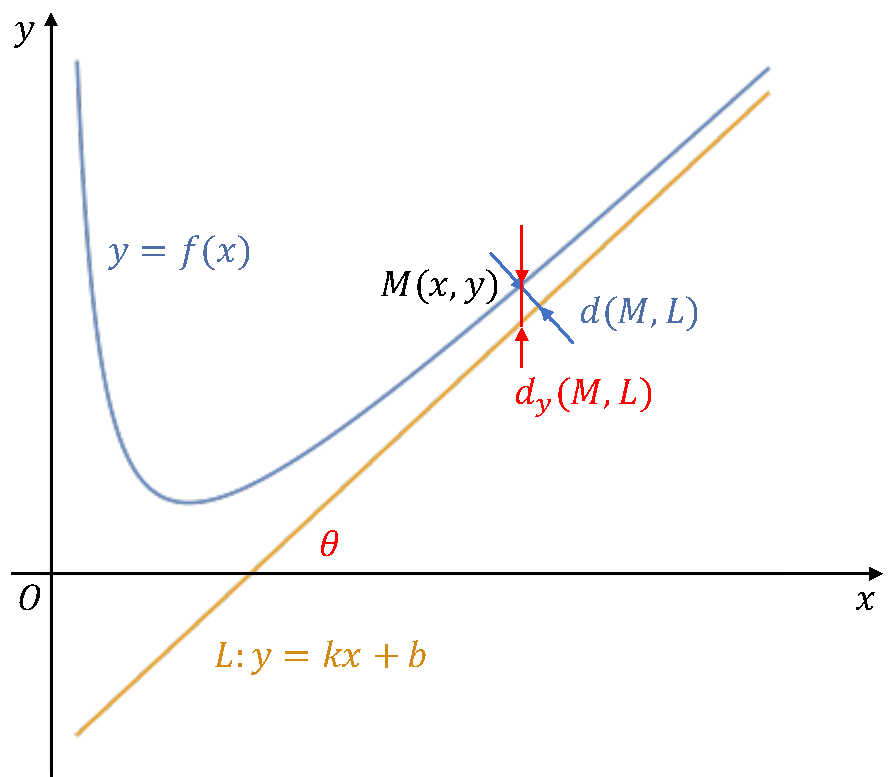
\includegraphics[width=0.45\textwidth]{./images/ch01/fkxb.pdf}
	\caption{斜渐近线}
	\label{fig:fkxb}
\end{figure}

先证必要性:如图\ref{fig:fkxb},显然
$$d(M,L)=d_y(M,L)\cos\theta,$$
其中$\theta=\arctan k$为常数,故$d(M,L)\to 0$当且仅当
$d_y(M,L)\to 0$。

由定义,直线$L:y=kx+b$为曲线$y=f(x)$当$x\to+\infty$时的渐近线,
当且仅当$x\to+\infty$时$d(M,L)\to 0$,也即$d_y(M,L)\to 0$,也即
$$\limx{+\infty}[f(x)-(kx+b)]=0.$$
等价于
$$\limx{+\infty}[f(x)-kx]=b.$$
进而可知
$$\limx{+\infty}\df{f(x)-kx}x=\limx{+\infty}\df bx=0.$$
也即
$$\limx{+\infty}\df{f(x)}x=k.$$

再证充分性。由$b=\limx{+\infty}[f(x)-kx]$,可知
$$\limx{+\infty}d_y(M,L)=\limx{+\infty}[f(x)-kx)]-b=0.$$
即证。

(2)由于
\pss{\centering
	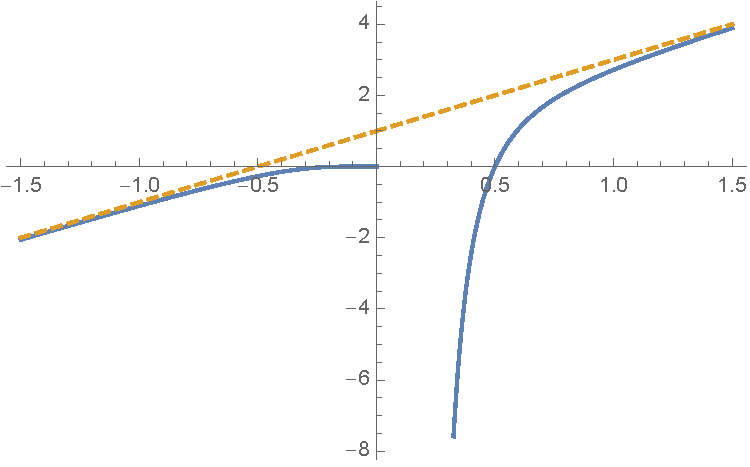
\includegraphics[width=0.9\marginparwidth]
	{./images/ch01/2x1e1x.pdf}\\
	$y=(2x-1)e^{\frac1x}$和它的斜渐近线
	$y=2x+1$
}
$$\limx{\infty}\df{(2x-1)e^{\frac1x}}x=2,$$
$$\limx{\infty}\left[(2x-1)e^{\frac1x}-2x\right]
=\limx{\infty}\left[2x(e^{\frac1x}-1)-e^{\frac1x}\right]
=\limx{\infty}2x\df1x-\limx{\infty}e^{\frac1x}=2-1=1,$$
故所求斜渐近线为$y=2x+1$。
\fin

\bs
接下来,我们暂时还不加证明地引入如下结论
\ps{后续章节中,我们将学习到因为初等函数在其定义区间内均连续,
故初等函数运算可以和极限运算交换次序}
\begin{thx}
	{\bf 定理:}初等函数运算可以和极限运算交换次序。
\end{thx}

\egz 计算极限
$$\limn\df{\cos^n\theta-\sin^n\theta}
{\cos^n\theta+\sin^n\theta}\quad
(0\leq\theta\leq\df{\pi}{2})$$

提示:根据$\theta$的取值范围,决定是分子分母同时除以$\sin^nx$还是$\cos^nx$,结果为
$$\mbox{原式}=\left\{\begin{array}{ll}
-1,& 0<\theta<\df{\pi}4\\
0,& \theta=\df{\pi}4\\
1,& \df{\pi}4<\theta<\df{\pi}2
\end{array}\right.$$
\fin

\egz 计算如下极限
\ps{处理{\it 无理分式}(包含非整数次幂的分式函数)
的常用技巧——{\it 分子有理化}}
\begin{enumerate}[(1)]
	\setlength{\itemindent}{1cm}
	\item $\limn\left(\sqrt{n+3\sqrt n}-\sqrt{n-\sqrt{n}}\right)$
	\item $\limn\left(\sqrt[3]{n^3+2n^2+1}-n\right)$
	\item $\limn\sin^2\left(\pi\sqrt{n^2+n}\right)$
\end{enumerate}

\ifhint
提示:
\begin{enumerate}[(1)]
	\setlength{\itemindent}{1cm}
	\item $\sqrt{n+3\sqrt n}-\sqrt{n-\sqrt{n}}
	=\df{\sqrt{n+3\sqrt n}+\sqrt{n-\sqrt{n}}}{4\sqrt{n}}$
	\item 利用公式$a^n-b^n=(a-b)(a^{n-1}+a^{n-2}b+\ldots+b^{n-1})$
	进行分子有理化:
	$$\mbox{原式}=\limn\df{2n^2+1}{(n^3+2n^2+1)^{\frac23}
	+(n^3+2n^2+1)^{\frac13}n+n^2}$$
	\item $\sin^2\left(\pi\sqrt{n^2+n}\right)
	=\sin^2\pi\left(\sqrt{n^2+n}-n\right)$,而
	$\limn\left(\sqrt{n^2+n}-n\right)=\frac{1}{2}$
\end{enumerate}
\fi

\bs
{\bf 课堂练习:}计算极限
\begin{enumerate}[(1)]
	\setlength{\itemindent}{1cm}
	\item $\limn\sqrt{n+\sqrt{n+\sqrt n}}-\sqrt n$
	\item $\limn(1+x)(1+x^2)\ldots(1+x^{2^n})$,其中$|x|<1$
\end{enumerate}

\ifhint
提示:
\begin{enumerate}[(1)]
	\setlength{\itemindent}{1cm}
	\item 分子有理化;
	\item 
	\begin{align*}
		&(1+x)(1+x^2)\ldots(1+x^{2^n})\\
		&=\df{(1-x)(1+x)(1+x^2)\ldots(1+x^{2^n})}{1-x}
		=\df{1-x^{2^{n+1}}}{1-x}
	\end{align*}
\end{enumerate}
\fi

\bs

{\bf 思考题:}
\begin{enumerate}[(1)]
	\setlength{\itemindent}{1cm}
	\item $\limn\left(1-\df1{2^2}\right)\left(1-\df1{3^2}
	\right)\ldots
	\left(1-\df1{n^2}\right)$
	\item $\limn\df32\cdot\df54\cdots\df{2^n+1}{2^n}$
\end{enumerate}

\ifhint
提示:
\begin{enumerate}[(1)]
	\setlength{\itemindent}{1cm}
	\item 因式分解,消去公共部分,结果$\frac{1}{2}$
	\item $\mbox{原式}=\limn2\left(1-\frac12\right)\left(1+\frac12\right)
	\left(1+\frac1{2^2}\right)
	\ldots\left(1+\frac1{2^n}\right)=2$
\end{enumerate}
\fi

\bs
{\bf 讨论:} 若$\limn x_n=a$,极限$\limn\df{x_{n+1}}{x_n}$是否一定存在?

\ifhint
答:不一定。反例:$x_n=\df1{3^{[n/2]}}$ (也即
$1, \df13, \df13, \df 1{3^2}, \df1{3^2}, \df1{3^3}, \df1{3^3},\ldots$)

请进一步思考,若$\limn x_n=a\ne 0$,则极限$\limn\df{x_{n+1}}{x_n}$
一定存在。为什么$a=0$时的结论就为不一定呢?
\fi

\subsection{复合函数的极限}

复合函数的极限需要分成多种情况来讨论:

\begin{thx}
	{\bf 复合函数的极限(情形I):}设
	$\limx{x_0}g(x)=u_0,\lim\limits_{u\to u_0}f(u)=A$,
	且在$x_0$附近$g(x)\ne u_0$,则
	$\limx{x_0}f[g(x)]=A.$
\end{thx}

证:对任意$\e>0$,由$\lim\limits_{u\to u_0}f(u)=A$可知,存在
$\delta_1>0$,对任意$u\in U_0(u_0,\delta_1)$,均有
$$|f(u)-A|<\e.$$
对以上的$\delta_1>0$,由$\limx{x_0}g(x)=u_0$,存在$\delta>0$,
使对任意$x\in U_0(x_0,\delta)$,均有
$$|g(x)-u_0|<\delta_1,$$
又由已知,在$x_0$附近$g(x)\ne u_0$,不妨设当$x\in U_0(x_0,\delta)$
时$g(x)\ne u_0$,从而可知此时$g(x)\in U_0(u_0,\delta_1)$,进而可得
$$|f(g(x))-A|<\e.$$
即证。\fin

\bs
{\bf 思考:}为什么定理条件中要求“在$x_0$附近$g(x)\ne u_0$”?

\bs
\ifhint
  答:因为$f(x)$可能在$x_0$处的定义与极限值无关,例如:
  $$f(x)=\left\{\begin{array}{ll}
  1,&x\ne0\\0,&x=0
  \end{array}\right.$$
  $g(x)\equiv 0$,则$f(g(x))\equiv0$,从而$\limx{0}f(g(x))=0$,
  而不是如定理所述$\limx{0}f(g(x))=1$。
\fi

直观的理解,以上的定理告诉我们:若相关极限都存在,且满足一定的条件,
则极限运算可以和函数运算交换次序。

在大多数的极限运算中,都会用到复合函数的极限运算。
例如:计算$\limx0\sin x^2$,这个极限显然等于$0$,
实际的计算过程应该是这样的:记$y=x^2$,注意到$\limx0y=0$,故
$$\limx0\sin x^2=\lim_{y\to0}\sin y=0.$$
或者可以这么看:
$$\limx0\sin x^2=\sin\left(\limx0x^2\right)
=\sin\left(\limx0x\right)^2
=\sin(0)^2=\sin0=0.$$

\bs
对于$x\to\infty$的情形,有类似的结论:
\begin{thx}
	{\bf 复合函数的极限(情形II):}设
	$\limx{+\infty}g(x)=u_0,\quad\lim\limits_{u\to u_0}f(u)=A,$
	且当$x$充分大时$g(x)\ne u_0$,则
	$\limx{+\infty}f[g(x)]=A.$

	{\bf 复合函数的极限(情形III):}设
	$\limx{x_0}g(x)=+\infty,\quad\lim\limits_{u\to+\infty}f(u)=A,$
	则
	$\limx{x_0}f[g(x)]=A.$
\end{thx}
想一想为什么最后这个命题似乎比前面的两个都少了一个条件?

\bs

{\bf 讨论:}判断与分析
\begin{enumerate}[(1)]
  \setlength{\itemindent}{1cm}
  \item 若$x\to x_0$时,$f(x)$有极限,$g(x)$无极限,则当$x\to x_0$时,以下哪些函数必无极限:
  $$f(x)g(x),\quad [g(x)]^2,\df{g(x)}{f(x)}, f(x)+g(x)$$ 
  \item 若$\limx{x_0}g(x)=A,\lim\limits_{u\to A}f(u)=B$,是否必有
  $\limx{x_0}f[g(x)]=B$?
  \item 若$\limx{x_0}f(x)g(x)=0$,则当$x\to
  x_0$时, $f(x),$ $g(x)$之一必趋于$0$.
\end{enumerate}

\ifhint
提示:
\begin{enumerate}[(1)]
  \setlength{\itemindent}{1cm}
	\item 不妨以$x\to0$时的极限为例:

	\quad$f(x)g(x)$可能收敛,例如:$f(x)=x,g(x)=D(x)$;

	\quad$[g(x)]^2$可能收敛,例如:$g(x)=\mathrm{sgn}(x)$;

	\quad$\df{g(x)}{f(x)}$必无极限。反证法:若该极限存在,则由极限的乘法规则
	$$\limx0g(x)=\limx0{g(x)}{f(x)}\limx0f(x)$$
	也存在,与已知矛盾;

	\quad$f(x)+g(x)$比无极限。证法与前一种情况类似。
	\item 错!反例:
	$$f(x)=\left\{\begin{array}{ll}
	  1,&x\ne0\\0,&x=0
	\end{array}\right.$$
	\quad$g(x)\equiv 0$,则$f(g(x))\equiv0$,
	从而$\limx{0}f(g(x))=0\ne 1$
	\item 错!反例:$f(x)=D(x)$,$g(x)=1-D(x)$,则$f(x)g(x)\equiv 0$。
	\fin
\end{enumerate}
\fi

{\bf 思考题:}设$\{a_n\},\{b_n\},\{c_n\}$均为非负数列,且
  $$\limn a_n=0,\quad \limn b_n=1,\quad \limn c_n=\infty.$$
  判断以下说法的正误。正确的,给出证明;错误的,举一个反例。
  \begin{enumerate}[(1)]
  	\setlength{\itemindent}{1cm}
    \item $n$充分大时,$a_n<b_n<c_n$;
    \item $\limn a_nc_n$必存在;
    \item $\limn b_nc_n$必不存在(极限为$\infty$属于极限不存在)。
  \end{enumerate}

\ifhint
提示:
\begin{enumerate}[(1)]
	\setlength{\itemindent}{1cm}
	\item 正确。利用极限的保号性证明即可。
	\item 错误。反例:$a_n=\frac1n,\;c_n=n^2$。
	\item 正确。利用极限的运算性质证明。
\end{enumerate}
\fi

\bs
\begin{ext}
	{\centering\bf 习题1-5}
	\begin{enumerate}  
	  \item 计算如下极限
	  \begin{enumerate}[(1)]
	    \item $\limx{1}\left(\df1{1-x}-\df3{1-x^3}\right)$
	    \item $\limx0\df{(h+x)^3-h^3}x$
	    \item $\limx{\infty}\df{\arctan x}{x^2}$
	    \item $\limx{+\infty}\df{\sqrt[3]{x+\sqrt{x+x^3}}}
	    {\sqrt{x+1}}$
	    \item $\limx4\df{\sqrt{2x+1}-3}{\sqrt{x-2}-\sqrt2}$
	    \item $\limx0\df{\sqrt[3]{x+1}-1}x$
	    \item $\limx0\df{\sqrt{1+x}+\sqrt{1-x}-2}{x^2}$
	    \item $\limx{+\infty}\df{\ln(2+e^{3x})}{\ln(3+e^{2x})}$
	    \item $\limx{+\infty}x(\sqrt{x^2+1}-x)$
	    \item $\limx{-\infty}x(\sqrt{x^2+1}-x)$
	    \item $\limx0x^2\sin\df1x$
	    \item $\limx{\infty}\df{\arctan x}x$
	  \end{enumerate}
	  \item 确定常数$a,b$的值,使得
	  $\limx{\infty}\left(\df{x^2}{x+1}-ax-b\right)=0$。
	\end{enumerate}
\end{ext}

\newpage
\section{极限存在准则与几个常用极限}

极限的基本运算法则,为计算极限提供了基本的方法。然而,有时,在判定
是否存在的过程中,仍有一些特殊的技巧,本节介绍的{\it 夹逼准则}
和{\it 单调有界准则}就是其中最常用的两个。

\subsection{夹逼准则}

夹逼准则也叫{\it 迫敛准则}或者{\it 三明治定理}。首先我们来看
针对数列极限的夹逼准则:
\begin{thx}
	{\bf 夹逼准则I:}设对任意$n\in\mathbb{N}$,$x_n\le a_n\le y_n$,
	且$\{x_n\},\{y_n\}$收敛于相同的极限$A$,则$\limn a_n=A$。
\end{thx}
证明略。

\begin{figure}[h]
	\centering
	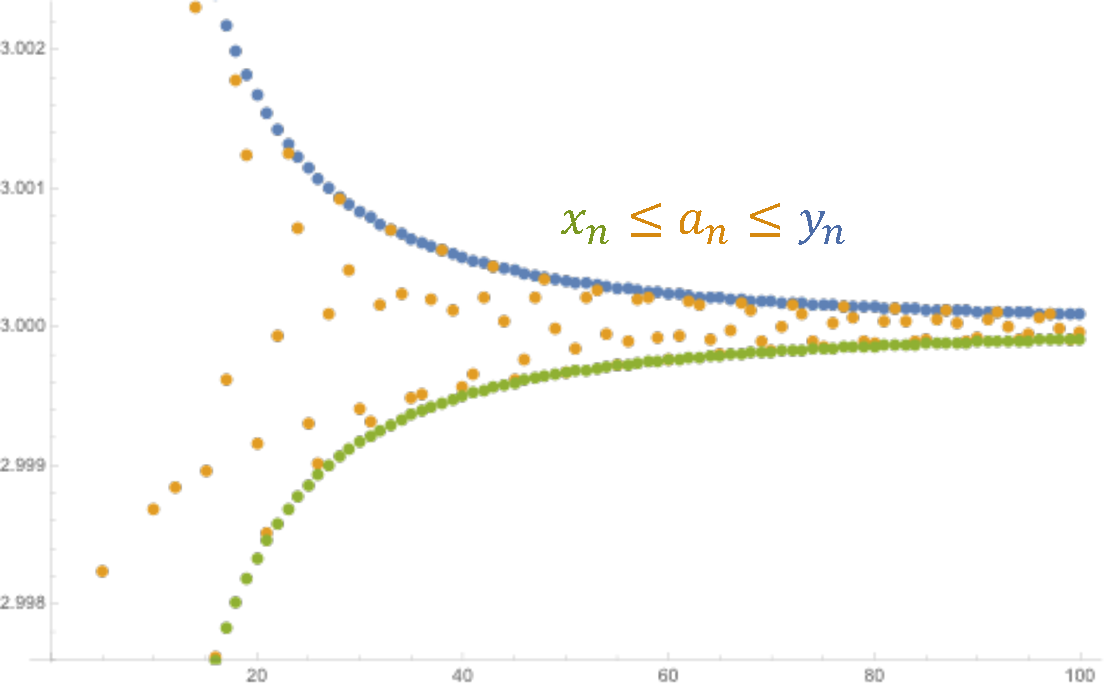
\includegraphics[width=0.6\textwidth]{./Images/Ch01/xnanyn.pdf}
	\caption{夹逼准则示意图}
	\label{fig:xnanyn}
\end{figure}

\bs

\egz 证明:$\limn (\sqrt{n+1}-\sqrt{n})=0$。

我们尝试分别用夹逼准则和极限的定义证明该定理。

证法一(夹逼准则):注意到
$$0<\sqrt{n+1}-\sqrt{n}={\df1{\sqrt{n+1}+\sqrt{n}}
\leq\df 1{\sqrt{n}}},$$
又
$$\limn 0=\limn\df 1{\sqrt{n}}=0,$$
故由夹逼准则,可知$\limn (\sqrt{n+1}-\sqrt{n})=0$。\fin

对比一下用定义证明的过程:

证法二(极限的定义):对任意$\e>0$,令$N=[1/\e^2]+1$,则对任意$n>N$,总有
$$\left|\sqrt{n+1}-\sqrt{n}-0\right|
={\df1{\sqrt{n+1}+\sqrt{n}}\leq\df 1{\sqrt{n}}}
<\df 1{\sqrt{N}}<\df 1{\sqrt{1/\e^2}}=\e,$$
由此可知$\limn (\sqrt{n+1}-\sqrt{n})=0$。\fin

不难发现,两个证明中最关键的放缩步骤是完全一致的,而使用夹逼准则时,可以直接
使用一些已知的或“简单的”极限结论,避免了推导$N$的繁琐步骤,因此过程显得更加
简洁也更容易理解。

\bs
{\bf 思考:}证明:$\limn [(n+1)^k-{n}^k]=0$,其中$0<k<1$。

\ifhint
提示:$n^k\left[\left(1+\df1n\right)^k-1\right]
<n^k\left(1+\df1n-1\right)=n^{k-1}\to 0\;(n\to\infty)$
\fi

\bs
\pss{\centering
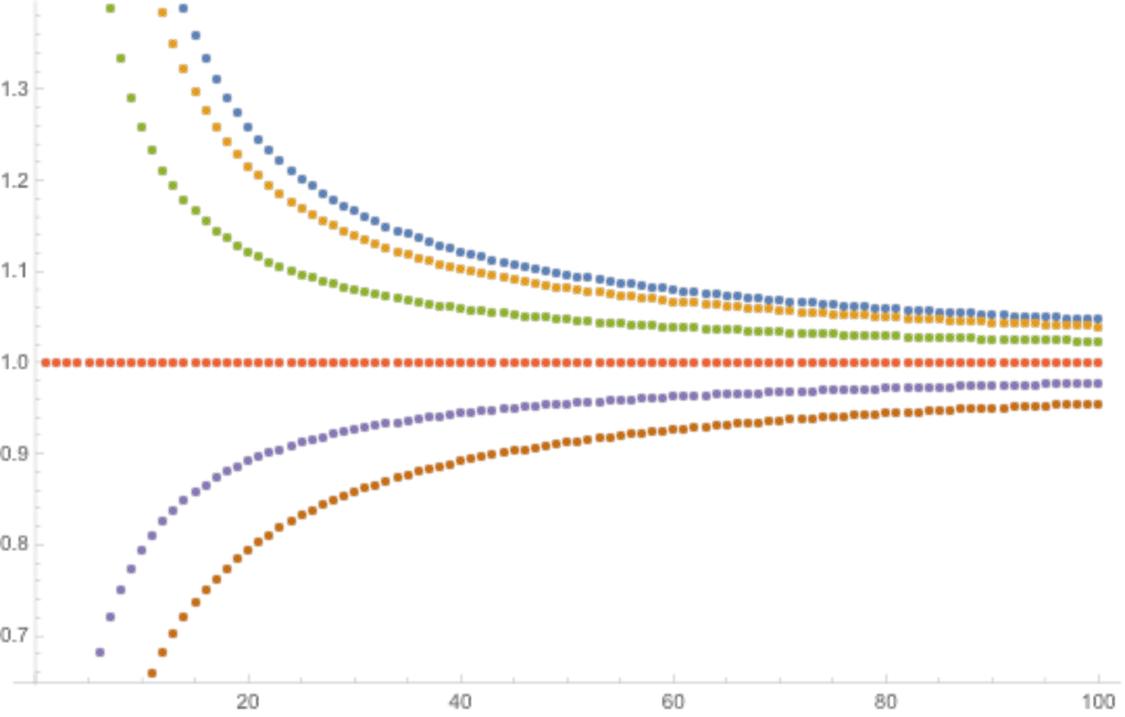
\includegraphics[width=0.9\marginparwidth]{./images/ch01/sqrtna.pdf}\\
不同$a$值(100,50,10,1,0.1,0.01)对应的数列$\{\sqrt[n]a\}$
}
\begin{thx}
	{\bf 常用极限:}若$a>0$为常数,则$\limn \sqrt[n]{a}=1$。
\end{thx}
证:$a=1$时结论显然成立。

$a>1$时,显然有$h_n=\sqrt[n]a-1>0$,故
$$a=(1+h_n)^n=1+nh_n+\df{n(n-1)}2h_n^2+\ldots+h_n^n>1+nh_n,$$
进而有
$$0<h_n<\df{a-1}n,$$
不等式左右两端当$n\to\infty$时极限均为$0$,故由夹逼准则,$\limn h_n=0$,也即
$$\limn\sqrt[n]a=1.$$

$0<a<1$时,令$b=\df1a$,则由极限的运算性质
$$\limn\sqrt[n]a=\limn\sqrt[n]{\df1b}
=\df1{\limn\sqrt[n]b}=\df11=1.$$
至此,证毕。\fin

利用本例类似的方法,可以证明:
\pss{\centering
	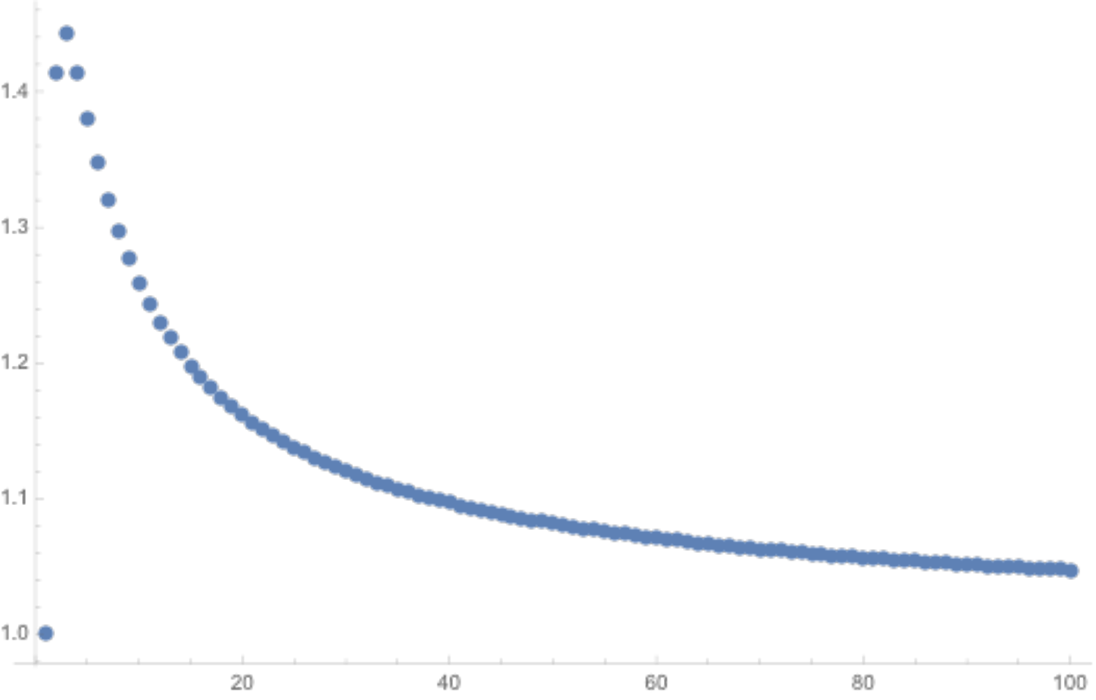
\includegraphics[width=0.9\marginparwidth]{./images/ch01/sqrtnn.pdf}\\
	数列$\{\sqrt[n]n\}$
	}
\begin{thx}
	{\bf 常用极限:}$\limn\sqrt[n]n=1.$
\end{thx}
请作为思考题加以练习。

\bs
{\bf 课堂练习:}计算极限
\begin{enumerate}[(1)]
  \setlength{\itemindent}{1cm}
  \item $\limn\sqrt[n]{n^5}$
  
  \ifhint \quad 提示:$\mbox{原式}=\left(\limn\sqrt[n]{n}\right)^5$.\fi
  \item $\limn\sqrt[n]{3^n+5^n}$.
  
  \ifhint \quad 提示:$5=\sqrt[n]{5^n}<\sqrt[n]{3^n+5^n}
  <\sqrt[n]{2\cdot 5^n}=\sqrt[n]2\sqrt[n]{5^n}=\sqrt[n]2\cdot5$.\fi
  \item $\limn\sqrt[n^2]{5^n+1}$
  \item 已知$a>b>0$,$\limn\sqrt[n]{\df1{a^n}+\df1{b^n}}$
  \item $\limn\df{\sqrt{n+\sqrt n}-\sqrt n}{\sqrt[n]{3^n+5^n+7^n}}$
  \item $\limn\left(\df1{n+1}+\df1{\sqrt{n^2+1}}+\ldots
	+\df1{\sqrt[n]{n^n+1}}\right)$
  \item $\limn n^2\left(\df kn-\df1{n+1}-\df1{n+2}
	-\ldots-\df1{n+k}\right),\;k\in\mathbb{Z}_+$
\end{enumerate}

以下例题中,我们多次用到了如下的常用极限:
\begin{thx}
  {\bf 常用极限:}设$a_k\geq0,\;(k=1,2,\ldots)$,则$\limn\sqrt[n]
  {\sum\limits_{k=1}^na_k^n}=\max\limits_{1\leq k\leq n}a_k.$
\end{thx}

\bs
夹逼准则可以很方便地推广到函数极限的情形,
\begin{thx}
	{\bf 夹逼准则II:}设在$\Delta$的某邻域内,恒有
	$$\varphi(x)\leq f(x)\leq\psi(x), $$
	且$\limx{\Delta}\varphi(x)=\limx{\Delta}\psi(x)=A$,则
	$$\limx{\Delta}f(x)=A.$$
\end{thx}

利用该准则,我们可以得到另一个常用的重要极限:
\pss{\baa 如未特别说明,以下三角函数中的$x$均取弧度值!}
\begin{thx}
	{\bf 常用极限:}$\limx{0}\df {\sin x}x=1$.
\end{thx}

证:如图,
	
\begin{figure}[h]
	\centering
	\includegraphics[width=0.35\textwidth]{./Images/Ch01/xsintan.pdf}
	\caption{三角不等式:$\sin\theta\leq\theta\leq\tan\theta,
	\;(\theta\geq0)$}
	\label{fig:xsintan}
\end{figure}
$\theta>0$时,显然弧$AB$的长度大于直线$BD$,即$\sin\theta<\theta$;
又扇形$ABO$的面积$\df12\theta$小于三角形$ACO$的面积$\df12\tan\theta$,
从而$\theta<\tan\theta$。由
$$\sin\theta<\theta<\tan\theta,$$
两边都除以$\sin\theta$,然后倒置,可得
$$1<\df{\sin\theta}{\theta}<\cos\theta,$$
注意到当$\theta\to 0^+$时,不等式左右极限都为$1$,故
$\lim\limits_{\theta\to0^+}\df{\sin\theta}{\theta}=1$。
又$\df{\sin x}x$为偶函数,故立即可得
$\lim\limits_{\theta\to0^-}\df{\sin\theta}{\theta}=1$。

综上即证。\fin

\begin{shaded}
	{\bf Cauchy的数列}

	在求解圆周率的计算过程中,诞生了一个重要的方法——割圆法。
	其基本思想是,如果用圆的内接正$n$边形来近似圆,则随着$n$的不断增大,
	二者周长和面积的误差将都越来越小,最终趋于零。

	据说,Cauchy给出了下面的数列:
	$$\{a_n\}=\left\{r^2n\cos\df{\pi}n\sin\df{\pi}n\right\}.$$
	不难验证该数列表示的是半径为$r$的正$n$边形的面积。利用极限
	$\limx0\df{\sin x}x=1$,不难验证:
	$$\limn a_n=\pi r^2\limn\df{\sin\frac{\pi}n}
	{\frac{\pi}n}\limn\cos\df{\pi}n=\pi r^2.$$
\end{shaded}

\bs
从这个极限出发可得到的一些常用的极限:

{\bf 课堂练习:}计算下列极限
\ps{\baa 这些极限的计算方法和结果都要熟记}
\begin{enumerate}[(1)]
	  \setlength{\itemindent}{1cm}
  \item $\limx{0}\df{\sin\sin x}{\sin x}$ 
  \item $\limx 0\df{1-\cos x}{x^2}$ 
  \item $\limx 0\df{\sin mx}{\sin nx}$
  \item $\limx 0\df{\tan x}{x}$
  \item $\limx 0\df{\arcsin x}x$
  \item $\limx 0\df{\arctan x}x$
  \item $\limx a\df{\sin x-\sin a}{x-a}$
\end{enumerate}

\ifhint
提示:
\begin{enumerate}[(1)]
	\setlength{\itemindent}{1cm}
	\item $\limx{0}\df{\sin\sin x}{\sin x}
	=\lim\limits_{y\to0}\df{\sin y}y=1$ 
	\item $\limx 0\df{1-\cos x}{x^2}
	=\limx 0\df{2\sin^2\frac x2}{x^2}
	=\limx 0\df12\df{\sin^2\frac x2}
	{\left(\frac x2\right)^2}=\df12$ 
	\item $\limx 0\df{\sin mx}{\sin nx}
	=\limx 0\df{\sin mx}{mx}\df{nx}{\sin nx}\df mn=\df mn$
	\item $\limx 0\df{\tan x}{x}
	=\limx 0\df{\sin x}{x}\limx0\cos x=1$
	\item $\limx 0\df{\arcsin x}x
	=\lim\limits_{y\to0}\df{y}{\sin y}=1$
	\item $\limx 0\df{\arctan x}x
	=\lim\limits_{y\to0}\df{y}{\tan y}=1$
	\item $\limx a\df{\sin x-\sin a}{x-a}
	=\limx a\df{\sin\frac{x-a}2\cos\frac{x+a}2}{\frac{x-a}2}=\cos a$
\end{enumerate}
\fi

\bs

\egz 设$f(x)=\sum\limits_{i=1}^na_i\sin
ix$,其中$a_i(i=1,2,\ldots,n)$为常数,且对任意$x\in\mathbb{R}$, $|f(x)|\leq |\sin x|$,证明:
$$\left|a_1+2a_2+\ldots+na_n\right|\leq 1$$

证:由已知,$x\ne 0$时,总有
$$\left|\df{f(x)}{\sin x}\right|\leq 1,$$
也即
$$\left|a_1+a_2\df{\sin 2x}{\sin x}+\ldots
+a_n\df{\sin nx}{\sin x}\right|\leq 1.$$
注意到对任意$k=2,3,\ldots,n$,总有$\limx{0}\df{\sin kx}{\sin x}=k$,
且对任意函数$f(x)$,由$\limx{0}f(x)=a$总可推出$\limx{0}|f(x)|=|a|$,故
在前式两边同时令$x\to0$,由极限的保号性可得
\begin{align*}
	|a_1&+2a_2+\ldots+na_n|
	=\left|a_1+a_2\limx0\df{\sin 2x}{\sin x}+\ldots
	+a_n\limx0\df{\sin nx}{\sin x}\right|\\
	&=\limx0\left|a_1+a_2\df{\sin 2x}{\sin x}+\ldots
	+a_n\df{\sin nx}{\sin x}\right|\leq 1,
\end{align*}
即证。\fin

\subsection{单调有界准则(原理)}

\pss{单调有界可以理解为单调递增有上界或单调递减有下界}
\begin{thx}
	{\bf 单调有界准则I:}单调有界
	数列必收敛。
\end{thx}

证:假设$\{a_n\}$单调递增有上界,由确界原理,可知其必有上确界,记为$A$。
以下证明$\limn a_n=A$。

事实上,对任意$\e>0$,由上确界的定义,必存在某个$a_N$,使得
$$A-\e<a_N\leq A.$$
又$\{a_n\}$单调递增,故对任意$n>N$,恒有$a_n\geq a_N$,
又$a_n\leq A$,从而
$$a_N\leq a_n\leq A\quad\Rightarrow\quad |a_n-A|<\e,$$
由极限的定义,即证。\fin

显然,以上证明中,完全可以不要求$\{a_n\}$是整体单调递增的,
有关的条件可以减弱为$\{a_n\}${\it 从某一项开始}
单调递增。

单调有界原理可以证明极限的存在性(或数列的收敛性),
但常常无法给出具体的极限值。例如下面的极限:

\pss{证明参见KD教材2.2.4节例7,不要求掌握}
\begin{thx}
	{\bf 常用极限:}$\left\{\left(1+\df1n\right)^n\right\}=e$.
\end{thx}

该极限结果的常数$e$称为{\kaishu Napier常数}
\ps{同济教材称之为Euler常数,
我们沿用的是维基百科和国际上通行的叫法;
Napier是公认的计算过程“机械化”的先驱},
以$e$为底的指数函数在微积分中有着非常广泛的应用。

\begin{shaded}
\egz 证明数列$\left\{\left(1+\df1n\right)^n\right\}$单调递增有上界。

证:先证有上界,
\begin{align}
	\left(1+\df1n\right)^n&=1+\df n1\cdot\df1n
	+\df{n\cdot(n-1)}{2\cdot1}\cdot\df1{n^2}+\ldots
	+\df{n\cdot(n-1)\ldots3\cdot2}{(n-1)\cdot(n-2)\ldots2\cdot1}\cdot\df1{n^2}\notag\\
	&<1+1+\df1{2\cdot1}+\ldots+\df1{(n-1)\cdot(n-2)\ldots2\cdot1}
	+\df1{n\cdot(n-1)\ldots2\cdot1}\notag\\
	&<1+1+\df12+\ldots+\df1{2^{n-2}}+\df1{2^{n-1}}<3\notag
\end{align}
再证单调性,由平均值不等式,
$$\left(1+\df1n\right)^n\cdot 1<
\left[\df{n\left(1+\frac1n\right)+1}{n+1}\right]^{n+1}
=\left(1+\df1{n+1}\right)^{n+1}.$$
\fin
\end{shaded}

需要了解和这个极限中的数列相关的一些重要性质:
\begin{itemize}
  \setlength{\itemindent}{1cm}
  \item 数列$\left\{\left(1+\df 1n\right)^n\right\}$严格单调递增有上界;
  \item 数列$\left\{\left(1+\df 1n\right)^{n+1}\right\}$严格单调递减有下界;
  \item 以上两个数列极限相同,都为$e$;显然
  $$\b\left(1+\df1n\right)^n<e<\left(1+\df1n\right)^{n+1}$$
\end{itemize}

\begin{figure}[h]
	\centering
	\includegraphics[width=0.6\textwidth]{./Images/Ch01/enn1.pdf}
	\caption{数列$\left\{\left(1+\df1n\right)^n\right\}$和数列
	$\left\{\left(1+\df1n\right)^{n+1}\right\}$}
	\label{fig:enn1}
\end{figure}

和这个极限相关的一类{\baa 典型错误:
\begin{eqnarray*}
	\limn\left(1+\df1n\right)^n&
	=&\limn \underbrace{\left(1+\df 1n\right)\left(1+\df 1n\right)\cdots
	\left(1+\df	1n\right)}_{n\mbox{\footnotesize\it 个}}\\
	&=&\underbrace{\limn\left(1+\df1n\right)\limn\left(1+\df1n\right)
	\cdots\limn\left(1+\df1n\right)}_{n\mbox{\footnotesize\it 个}}\\
	&=&\left[\limn\left(1+\df1n\right)\right]^n=1
\end{eqnarray*}}
和前面关于无穷多个无穷小的和的例子类似,这样相当于把某个$n$
放在了极限符号之外,而且,不要忘记,极限运算只能和有限次的四则
运算交换次序(否则结果可能是不确定的)。

\begin{shaded}
	{\bf Napier常数$e$}

	关于Napier常数$e$有如下的一些结论(在此不作证明):	
	\begin{itemize}
		\setlength{\itemindent}{1cm}
		\item 若将$a>0$分成若干份,使得总乘积最大,由平均值不等式可知,
		显然等分最有利,但该分成多大的一份呢?分析可证明分成最接近
		于$e$的大小最合适;
		\item 记$\e_n=e-\sum\limits_{k=0}^n\df1{k!}$,则
		\limn $e_n(n+1)!=1$;
		\item $\delta_n=e-\left(1+\df1n\right)^n<\df3n$;
		\item $\limn\df{2n\delta_n}e=1$;
		\item $\df1{n+1}<\ln\left(1+\df1n\right)<\df1n$;
		\item $a_n=\df1{n+1}+\ldots+\df1{2n},\;(n\in\mathbb{Z}_+)$收敛
		于$\ln2$.
	\end{itemize}
	
	\bs
	{\bf Euler常数}
	$$\gamma=\limn\left(\sumn\df1k-\ln n\right)\approx 0.5772\ldots$$
\end{shaded}

利用前述的性质,结合夹逼准则,我们可以推广以上的极限得到:
\begin{thx}
	{\bf 常用极限:}$\limx{\infty}\left(1+\df1x\right)^x=e.$
\end{thx}

证:先证明$\limx{+\infty}\left(1+\df1x\right)^x=e$。

以下$[x]$表示对$x$下取整。

对任意$x>0$,显然$[x]\leq x<[x]+1$,于是由前述的重要不等式
$$\left(1+\df1n\right)^n<e<\left(1+\df1n\right)^{n+1},$$
可得
$$\left(1+\df1{[x]+1}\right)^{[x]}<\left(1+\df1x\right)^x
<\left(1+\df1{[x]}\right)^{[x]+1}.$$
利用前述极限容易证明以上不等式两边的数列极限均为$e$,从而由夹逼准则,
$\limx{+\infty}\left(1+\df1x\right)^x=e$。

下证$\limx{-\infty}\left(1+\df1x\right)^x=e$。

事实上,记$y=-x$,则
\begin{align*}
	\limx{-\infty}\left(1+\df1x\right)^x
	&=\lim\limits_{y\to+\infty}\left(1-\df1y\right)^{-y}
	=\lim\limits_{y\to+\infty}\df1{\left(1-\df1y\right)^{y}}\\
	&=\lim\limits_{y\to+\infty}\left(\df y{y-1}\right)^{y}
	=\lim\limits_{y\to+\infty}\left(1+\df1{y-1}\right)^{y}\\
	&=\lim\limits_{y\to+\infty}\left(1+\df1{y-1}\right)^{y-1}
	\lim\limits_{y\to+\infty}\left(1+\df1{y-1}\right)=e\cdot1=e
\end{align*}
\fin

\bs
从以上极限出发也可以得到的一些常用的极限:

\egz 计算如下的极限\ps{\baa 重点掌握}
\begin{enumerate}[(1)]
   \setlength{\itemindent}{1cm}
  \item $\limx{0}(1+x)^{1/x}$ 
  \item $\limx 0(1+\sin x)^{1/\sin x}$ 
  \item $\limx 0\df{\ln(1+ax)}{x}=a$
  \item $\limx 0\df{e^{ax}-1}{x}=a$ 
  \item $\limx 0\df{a^x-1}{x}=\ln a$ 
  \item $\limx 0\df{(1+x)^a-1}x=a$
  \item $\limn n(\sqrt[n]{a}-1)=\ln a$ 
\end{enumerate}

\ifhint
提示:
\begin{enumerate}[(1)]
	\setlength{\itemindent}{1cm}
	\item $\limx{0}(1+x)^{1/x}
	\xlongequal{y=\frac1x}
	\lim\limits_{y\to\infty}\left(1+\df1y\right)^y=e$ 
	\item $\limx 0(1+\sin x)^{1/\sin x}
	\xlongequal{y=\sin x}\lim\limits_{y\to0}\left(1+y\right)^y=e$ 
	\item $\limx 0\df{\ln(1+ax)}{x}
	=a\limx0\ln(1+ax)^{\frac1{ax}}=a$
	\item $\limx 0\df{e^{ax}-1}{x}=a
	\xlongequal{y=e^{ax}-1}
	\lim\limits_{y\to0}\df{y}{\frac1a\ln(1+y)}=a$ 
	\item $\limx0\df{a^x-1}{x}
	=\limx0\df{e^{x\ln a}-1}x=\ln a$ 
	\item $\limx0\df{(1+x)^a-1}x
	=\limx0\df{}{e^{a\ln(1+x)}-1}{\ln(1+x)}
	\cdot\df{\ln(1+x)}x=a$
	\item $\limn n(\sqrt[n]{a}-1)
	\xlongequal{x=\frac1n}
	\limx0\df{a^x-1}x=\ln a$ 
\end{enumerate}
\fi

\bs
\egz 设$f(x)$在$[a,b]$上连续,$\{x_n\}$为$[a,b]$上任一数列,求
$\limn\sqrt[n]{\df1n\sum\limits_{k=1}^ne^{f(x_k)}}$

解:$e^{f(x)}$在$[a,b]$上连续且非负,故可设
$m,M$分别为其在$[a,b]$上的最大和最小值,
\ps{这里用到了连续函数的性质,即:有界闭区间上的连续函数必可以去到最大
和最小值}
从而由夹逼定理
$$\sqrt[n]m\leq\sqrt[n]{\df1n\sum\limits_{k=1}^ne^{f(x_k)}}\leq\sqrt[n]M,$$
由此易知原式$=1$。\fin

\bs
单调有界准则一个很常见的应用领域时判断递推数列的敛散性。

\egz 
设$a_1>0$,$a_{n+1}=\df 12\left(a_n+\df 1{a_n}\right)\,
(n=1,2,\ldots)$,证明$\{a_n\}$收敛,并求其极限。

解:显然对任意$n\in\mathbb{Z}_+$,均有$a_n>0$。
又对任意$n\geq2$,由平均值不等式,
$$a_n=\df 12\left(a_n+\df 1{a_n}\right)\geq 1.$$
进而$\df1{a_n}\leq a_n$,从而
$$a_{n+1}-a_n=\df12\left(\df1{a_n}-a_n\right)\leq0.$$
由此即知,从$a_2$开始,数列$\{a_n\}$单调递减有下界,
从而由单调有界准则,$\{a_n\}$必收敛。

设$\limn a_n=A$,在递推式两边取极限,可得
$$A=\df12\left(\df1A+A\right)\quad\Rightarrow\quad A=\pm1.$$
由极限的保号性,显然$A\geq0$,故$A=1$,即为所求。\fin

{\bf 思考:}是否可以考虑使用单调有界准则证明递推数列的极限存在,有一个简单的
分析判断方法:先假设极限存在,然后在递推式两边同时取极限,若由此可以
解出极限,则可以考虑使用单调有界来验证极限存在(逻辑上,应该是
先验证极限存在,再计算它)。然后有些时候,两边取极限后,无法解出
极限的值,或者关于极限值的方程无解,请思考这两种情况分别意味着什么?
又应该如何进行处理?

\ifhint
答:如果无法解出极限的值,例如这样的递推式
$$a_{n+1}=\df12(a_n+a_{n-1}),$$
则应考虑从递推式出发,求出数列的通项公式(参见下面的例题);
而如果关于极限值的方程无界,则意味着该极限必不存在!
\fi

\bs
\egz 已知$a_1,a_2$为常数,数列$\{a_n\}$满足:
$$a_n=\df 12({a_{n-1}+a_{n-2}})\quad(n>2).$$
证明$\{a_n\}$收敛,并求其极限。

解:原递推式可改写为
$$a_n-a_{n-1}=-\df12(a_{n-1}-a_{n-2})\quad(n>2),$$
由此递推,易得
$$a_n-a_{n-1}=\left(-\df12\right)^{n-2}(a_2-a_1),$$
进而
\begin{align}
	a_n&=a_{n-1}+\left(-\df12\right)^{n-2}(a_2-a_1)\notag\\
	&=a_{n-2}+\left[\left(-\df12\right)^{n-3}+\left(-\df12\right)^{n-2}\right]
	(a_2-a_1)\notag\\
	&=\ldots\notag\\
	&=a_2+\left[\left(-\df12\right)+\ldots+\left(-\df12\right)^{n-3}
	+\left(-\df12\right)^{n-2}\right](a_2-a_1)\notag\\
	&=a_2-\df12\df{1-\left(-\df12\right)^{n-2}}{1+\df12}(a_2-a_1)\notag\\
	&\to\df13a_1+\df23a_2\;(n\to\infty)\notag
\end{align}
即证。\fin

\begin{shaded}
	{\bf 特征根法求解求解二阶常系数齐次递推}

	中学阶段,有些同学接触过所谓的特征根法求递推公式,具体过程如下,其背后
	的原理与上面一个例子中的方法是完全一致的。

	已知$a_1,a_2$和如下的递推式:

	$$a_{n+2}=Aa_{n+1}+Ba_n\quad (AB\ne 0, A+B\ne 1),$$
	求$\{a_n\}$的通项公式。

	考虑特征方程:
	$$r^2=Ar+B$$
	\begin{enumerate}[(1)]
	  \setlength{\itemindent}{1cm}
	  \item 若特征方程有相异实根$p,q$,则
	  $$a_n=C_1p^n+C_2q^n$$
	  其中系数$C_1,C_2$由方程
	  $$\left\{\begin{array}{l}
	  a_1=C_1p+C_2q\\
	  a_2=C_1p^2+C_2q^2
	  \end{array}\right.$$
	  可解得
	  $$C_1=\df{a_1q-a_2}{p(q-p)},\quad
	  C_2=\df{a_1p-a_2}{q(p-q)}$$
	  \item 若有两个相等的实根$r$,则
	  $$a_n=[C_1r+C_2(n-1)]r^{n-1}$$
	  与(1)类似地可求出系数$C_1,C_2$
	\end{enumerate}

	例如,Fibonacci数列:$a_{n+2}=a_n+a_{n+1},\;a_1=a_2=1$,
	按照以上方法,可求得
	$$a_n=\df1{\sqrt5}\left[\left(\df{1+\sqrt5}2\right)^n
	-\left(\df{1-\sqrt5}2\right)^n\right]$$
\end{shaded}

\bs
\egz 证明极限$\limn\df{n^2}{a^n}\quad (a>1)$存在,然后求其值。

解:记$b_n=\df{n^2}{a^n}$,则
$$b_{n+1}=\df{(n+1)^2}{n^2a}b_n,$$
注意到$\limn\df{b_{n+1}}{b_n}=\df1a<1$,故当$n$充分大时,
$\{b_n\}$严格单调递减,
而显然$b_n>0$,故由单调有界原理,$\{b_n\}$收敛,
设其极限为$A$。在前述递推式两端同时取极限,
可得
$$A=\df1aA\quad\Rightarrow\quad A=0,$$
即为所求。\fin

本例中的极限也是一个常用极限,可以更一般地写为
\begin{thx}
	{\bf 常用极限:}对任意$m\in\mathbb{R}$和任意$a>1$,总有
	$\limx{+\infty}\df{x^m}{a^x}=0$。
\end{thx}
这个极限的意思可以形象地解释为“随着$x$不断增大,幂次再高的幂函数相对于
一个底数超过$1$的指数函数而言,都是微不足道的”!试着利用该极限证明:

{\bf 课堂练习:} 证明:$\limn\sqrt[n]{n^5+5^n}=5$。

\bs
再来看一个递推数列极限不存在的例子:

\egz $x_1=\df c2$,$x_{n+1}=\df c2+\df{x_n^2}2\,(n\in\mathbb{Z}_+)$,
证明:若$c>1$,则$\{x_n\}$发散。

证:设极限为$A$,则$A^2-2A+c=0$,$c>1$时,无解,必发散。\fin

\bs
递推数列的问题对很多人来说是学习的难点,这部分需要多加练习:

\bs
{\bf 思考:} $a_0>b_0>0$,
$$a_n=\df12(a_{n-1}+b_{n-1}),\quad
b_n=\sqrt{a_{n-1}b_{n-1}}\;(n\in\mathbb{Z}_+)$$
证明:$\{a_n\},\{b_n\}$收敛于同一极限。

\ifhint
提示:$b_0<b_1<a_1<a_0$,利用数学归纳法证明:
$$b_0<b_1<\ldots<b_n<a_n<\ldots<a_1<a_0$$
\fi

\bs
{\bf 思考:}证明:$a_n=\sqrt{1+\sqrt{2+\ldots+\sqrt{n}}}$收敛。

\ifhint
提示:注意到
$$\sqrt{n-1+\sqrt n}<\sqrt{n-1+2\sqrt{n-1}+1}=\sqrt{n-1}+1,$$
然后利用不等式$\sqrt{n-1}<2\sqrt{n-2}$递推。
\fi

\bs
{\bf 思考:}给定$x\in(0,3),\; x_{n+1}=\sqrt{x_n(3-x_n)},
\;(n\in\mathbb{Z}_+)$,
证明数列$\{x_n\}$收敛,并求其极限。

\ifhint
提示:$0<x_2\leq\df12[x_1+(3-x_1)]=\df32$,递推可得
$0<x_n\leq\df32$。另一方面,
$$x_{n+1}-x_n=\df{\sqrt{x_n}(3-2x_n)}{\sqrt{x_n(3-x_n)}
+\sqrt{x_n}}\geq 0.$$
即$\{x_n\}$单调递增有上界。
\fi

\bs
{\bf 思考:}证明数列$\{x_n\}:x_1=1,\;x_{n+1}
=\df1{1+x_n}$收敛,求其极限。

\ifhint
提示:由递推式易得极限$a=\df{\sqrt5-1}2$。(写成:$a$为满足方程$a=\df1{1+a}$的正数)

显然$0<x_n\leq1$,进而$\df1{1+x_n}\geq\df12$。于是\ps{$\{x_n\}$不单调!}
\begin{align}
	|x_{n+1}-a|&=\left|\df1{1+x_n}-\df1{1+a}\right|=\df{|x_n-a|}{(1+x_n)(1+a)}\notag\\
	&<\df{|x_n-a|}{(1+1/2)(1+1/2)}=\df49|x_n-a|\notag\\
	&<\left(\df49\right)^2|x_{n-1}-a|<\ldots<\left(\df49\right)^{n}|x_1-a|,\notag
\end{align}
由夹逼定理可知$|x_{n+1}-a|\to0\;(n\to\infty)$,即证。
\fi

\bs
{\bf 思考:}设$a_1\in(0,2)$,$(2-a_n)a_{n+1}=1\,(n=1,2,\ldots)$,证明:
数列$\{a_n\}$收敛,并求其极限。

\ifhint
证法一:若存在某个$a_{n_0}=1$,则可知对任意$n\geq n_0$必有$a_n=1$,
此时数列$\{a_n\}$收敛,极限为$1$。

若不存在任何一个$a_n=1$,则可令$b_n=\df1{1-a_n}$,由已知等式可得
$$b_{n+1}=1+b_n=2+b_{n-1}=\ldots=n+b_1,$$
进而可得
$$a_n=1-\df1{b_n}=\df{n-2+b_1}{n-1+b_1}\to 1,\;(n\to\infty).$$
即证。\fin

这个方法需要很强的观察和构造能力,且并不容易推广,使用起来有一定的难度。
下面的方法,需要结合$a_1$的不同取值,进行更为复杂的讨论,但相对而言
不需要进行任何构造,难度略微降低了一些。

证法二:
\begin{center}
	\includegraphics[width=8cm]{./images/ch01/a2a.pdf}
	
	\it 给定不同的$a_1$,数列取值的变化规律
	
	可以看到,不论$a_1$如何取,当$n$充分大时,数列都是单调递增有上界的
\end{center}

若存在某个$a_{n_0}=1$,则可知对任意$n\geq n_0$必有$a_n=1$,
此时数列$\{a_n\}$收敛,极限为$1$。

排除以上的情况,对剩余的可能进行讨论。

(1)存在某个$a_{n_0}\in(0,1)$,显然,由$a_{n+1}=\df1{2-a_n}$
可知,对任意$n\geq n_0$时均有$a_n\in(0,1)$,进而
$$a_{n+1}-a_n=\df{(1-a_n)^2}{2-a_n}>0,$$
综上,当$n>n_0$时,数列$\{a_n\}$单调递增有上界,从而收敛;

(2)存在某个$a_{n_0}\in(1,2)$,显然,$a_{n_0+1}>1$,
且对$n\geq n_0$,只要$a_n<2$,都有$a_{n+1}-a_n>0$,若
最终所有的$a_n$都小于$2$,则由单调有界原理,可知$\{a_n\}$
收敛;

(3)存在某个$a_{n_0}>2$,则必有$a_{n_0+1}<0$,
进而必有$a_{n_0+2}\in(0,1)$,于是由前述情况(1)
的讨论可知,当$n\geq n_0+2$时,数列$\{a_n\}$单调递增有上界,从而收敛;

(4)存在某个$a_{n_0}<0$的情况,已经包含在上述
情况(3)的讨论中,故此时$\{a_n\}$也收敛。

综上,数列$\{a_n\}$必收敛。设其极限为$A$,在以上等式两边同时令$n\to\infty$,可得
$(2-A)A=1$,解得$A=1$,即为$\{a_n\}$的极限。\fin
\fi

总结一下
\begin{thx}
	{\bf 求解递推数列的极限问题的几个要点:}
	\begin{itemize}
% 	  \setlength{\itemindent}{1cm}
	  \item 递推式两边同时取极限,解方程求得极限的值,是最便利的计算递推数列极限的方法
	  \item 若通过以上方法可以求出极限的值,通常只需证明数列单调有界即可
	  \item 若该方法无法求得极限的值,则只能利用递推式推导数列通项,进而证明其收敛并计算极限
	\end{itemize}
\end{thx}

\bs
最后,给出函数极限对应的单调有界准则:
\begin{thx}
{\bf 单调有界准则II:}设$f(x)$当$x$从单侧趋于$\Delta$
时单调且有界,则$\limx{\Delta}f(x)$存在。
\end{thx}

例如:若$f(x)$在$x_0$的某个左邻域内单调递增且有上界,则$f(x_0-0)$存在;
若$f(x)$当$x$充分大时单调递减且有下界,则$f(+\infty)$存在。

\begin{shaded}
\subsection{Cauchy极限存在准则}

\pss{\centering
	\includegraphics[width=0.7\marginparwidth]{./images/ch01/200px-Augustin-Louis_Cauchy_1901.jpg}\\
	\href{https://en.wikipedia.org/wiki/Karl_Weierstrass}
	{A. L. Cauchy(1789-1857)}\\
	在现代数学的各个分支中,随处可见他的诸多贡献
}
\begin{thx}
{\bf Cauchy审敛原理:}
数列$\{a_n\}$收敛,当且仅当:对任意$\e>0$,存在正整数$N$,使对任意$m,n>N$,总有
$$|a_m-a_n|<\e.$$
\end{thx}

Cauchy收敛准则的必要性容易证明,但充分性的证明时相当复杂的,这里不作介绍,
感兴趣的可以查阅菲赫金哥尔茨的《微积分学教程》。

\bs
\egz 证明$a_n=1+\df12+\df13+\ldots+\df1n$发散。

这里我们要用到Cauchy审敛准则的反面说法:数列$\{a_n\}$发散,当且仅当:存在$\e_0>0$,
使对任意的正整数$N$,都存在$m_0,n_0>N$,使得
$$|a_{m_0}-a_{n_0}|\geq\e_0.$$

证:取$\e_0=\df12$,则对任意的正整数$N$,总可以取$m_0=N,n_0=2N$,则
\begin{align*}
	|a_{m_0}-a_{n_0}|
	&=\df1{N+1}+\df1{N+2}+\ldots+\df1{2N}\\
	&>\underbrace{\df1{2N}+\df1{2N}\ldots+\df1{2N}}
	_{N\mbox{\footnotesize 个}}=\df12=\e_0,
\end{align*}
即证。\fin

\subsection{Stolz定理}

\begin{thx}
	{\bf Stolz定理:}
	($\df{\bm{\infty}}{\bm{\infty}}$型) 设数列$\{y_n\}$满足$\limn\df
	1{y_n}=0$,且$\{y_n\}$至少从某一项开始保持严格单调递增,
	则对任意数列$\{x_n\}$,若$\limn\df{x_n-x_{n-1}}{y_n-y_{n-1}}$存在,则必有
	$$\limn\df{x_n}{y_n}=\limn\df{x_n-x_{n-1}}{y_n-y_{n-1}}$$
\end{thx}

Stolz定理类似于函数极限中的L'Hospital法则,例如:
对比$\limn\df{n^2}{e^n}$和$\limx{+\infty}\df{x^2}{e^x}$。

不难验证,此前介绍过的Cauchy极限(命题)是Stolz定理的一个推论。

\bs
\egz 计算以下极限
\begin{enumerate}[(1)]
  \setlength{\itemindent}{1cm}
  \item $\limn\df{1+\sqrt 2+\sqrt[3]{3}+\ldots+\sqrt[n]{n}}{n}$ 
  \item $\limn\df{1!+2!+\ldots+n!}{n!}$
  \item $\limn\df{\ln n}{1+\frac12+\ldots+\frac1n}$
\end{enumerate}

\bs
\egz  设$\limn a_n=a$,证明:
\begin{enumerate}[(1)]
  \setlength{\itemindent}{1cm}
  \item $\limn\df{a_0+a_1+\ldots+na_n}{n^2}=\df a2$
  \item $\limn\df{a_1+\frac12a_2+\ldots\frac1na_n}{\ln n}=a$
\end{enumerate}

\bs
由Cauchy极限(命题),进一步可以得到如下两个推论:

\begin{thx}
{\bf 推论1:}设$\{a_n\}$为正数列,则
$\limn\sqrt[n]{a_1a_2\ldots a_n}=\limn a_n$

{\bf 推论2:}设$\{a_n\}$为正数列,$\limn\df{a_{n+1}}{a_n}=q$,
则$\limn\sqrt[n]{a_n}=q$
\end{thx}

\bs
\egz 计算极限$\limn\df{\sqrt[n]{n!}}{n}$

提示:记$b_n=\df{n!}{n^n}$,则由以上推论
$$\limn\sqrt[n]{b_n}=\limn\df{b_{n+1}}{b_n}=\df1e$$

\bs
\egz 设$a>1$,证明:$\limn\df{n}{a^n}=0$。

提示:由Stolz定理,
$$
	\limn\df{n}{a^n}=\limn\df1{a^n-a^{n-1}}
	=\limn\df1{a-1}\df1{a^{n-1}}=0.
$$
事实上,这个结论可以很容易地推广到:$\limn\df{n^k}{a^n}=0$,其中
$a>1$,$k$为任意的常数。

\bs
Stolz定理还有另一种形式:
\begin{thx}
	{\bf Stolz定理}($\df00$型)设$\limn a_n=\limn b_n=0$,且$\{a_n\}$严格
	单调递减,若$\limn\df{b_{n+1}-b_n}{a_{n+1}-a_n}=l$($l$可以为$\pm\infty$),
	则$\limn\df{b_n}{a_n}=l$
\end{thx}
\end{shaded}

\begin{ext}
	{\centering\bf 习题1-6}
	
	\begin{enumerate}  
	  \item 计算下列极限
	  \begin{enumerate}[(1)]
	    \item $\limx{\pi}\df{\sin 7x}{\cos 4x}$
	    \item $\limx0\df{(1+x)^{1+x}+x\sin\df1x}{e^x+\sin x}$
	    \item $\limx{a}\df{\cos x-\cos a}{x-a}$
	    \item $\limx0\df{1-\cos3x}{x\sin x}$
	    \item $\limx1\df{x-1}{\sqrt{x+3}-2}$
	    \item $\limx1\df{\sqrt[3]x-1}{\sqrt x-1}$
	    \item $\limn\left(1+\df1n\right)^{n-6}$
	    \item $\limn\left(\df{n}{n^2+1}+\df{n}{n^2+2}
	    +\ldots+\df{n}{n^2+n}\right)$
	    \item $\limx0(1-x)^{\frac1{\sin x}}$
	    \item $\limx{\infty}\left(\df{1+x}{2+x}\right)^{2x}$
        \item $\limx{+\infty}\left(\df{1+x}{1+2x}\right)^{2x}$
	  \end{enumerate}
	  \item 证明数列
	  $$a_n=\underbrace{\sqrt{2+\sqrt{2+\ldots+\sqrt2}}}
	  _{n\mbox{\footnotesize 个}2}$$
	  收敛,并求其极限。
	  \item 已知$A_1+A_2+\ldots+A_k=0$,证明
	  $$\limn (A_1\sqrt{n+1}+A_2\sqrt{n+2}+\ldots+A_k\sqrt{n+k})=0.$$
	  \item 求$f(x)=\sqrt[n]{1+x^n+\left(\df{x^2}2\right)^n}$($x\geq 0$)
	  的分段表达式。
% 	  \begin{enumerate}[(1)]
% 	    \item $\limx{1}\left(\df1{1-x}-\df3{1-x^3}\right)$;
% 	    \item $\limx0\df{(h+x)^3-h^3}x$;
% 	    \item $\limx{\infty}\df{\arctan x}{x^2}$。
% 	  \end{enumerate}
	  \item (选作)设$|\lambda|<1$,计算
	  $\limn(\lambda+2\lambda^2+\ldots+n\lambda^n)$ 
	\end{enumerate}
\end{ext}

\newpage
\section{无穷小的比较}

在极限的计算问题中,真正困难的问题都是一些所谓的“{\it 不定式}”
或“{\it 不定型}”极限。比如:
$$\limx{a}\df{\sin x-\sin a}{x-a},\quad \limx{0}(1+\tan x)^{\cot x},
\quad \limn n(\sqrt[n]2-1).$$
之所以称之为“不定”,是相对于一些“确定”的函数形式而言的,例如:
$$\limx{0}\df{x}{1+x^2},\quad \limx{0}(1+\tan x)^{\tan x},
\quad \limn\df{2}{1+n^2}.$$
这三个例子都可以直接利用极限的运算性质来进行计算:
\begin{align*}
	&\limx{0}\df{x}{1+x^2}=\df{\limx{0} x}{1+\limx{0}x^2}=\df0{1+0}=0\\
	&\limx{0}(1+\tan x)^{\tan x}=(1+\limx{0}\tan x)^{\limx{0}\tan x}
	=(1+0)^0=1\\
	&\limn\df{2}{1+n^2}=0
\end{align*}
而从函数的构造形式上看,它们可以分别称为$\df{\bm{0}}{\bm{1}},\bm{1^0}$
\ps{这里的$\bm{0},\bm{1},\bm{\infty}$分别代表极限对应过程中的
无穷小、有界量和无穷大}和
$\df{\bm{1}}{\bm{\infty}}$型的,只要是具有类似这样的构造形式,其结果就是确定的
$0,1$和$0$。

作为对比,如果观察最初的三个例子,根据其结构特点可以分别称为是
$\df{\bm0}{\bm0},\bm{1^{\infty}}$
和$\df{\bm{\infty}}{\bm{\infty}}$型的,
类似这样的极限一个最大的特点是,仅仅从这样的结构特点上,很难直接看出极限的值。
以$\df{\bm0}{\bm0}$型的极限为例:
$$\limx{0}\df{\sin x}x=1,
\quad \limx{0}\df{\sin x^2}x=0,
\quad \limx{0}\df{1-\cos x}{x^2}=\df12,$$
虽然结构类型一样,但结果却各不相同。

类似这样的结构,如果稍加总结,一共包含如下的一些类型,它们之间的转换关系如图所示:
	
\begin{figure}[h]
	\centering
	\includegraphics[width=0.5\textwidth]{./Images/Ch01/lim00.pdf}
	\caption{不定式(型)极限之间的转换关系}
	\label{fig:lim00}
\end{figure}

既然不定式极限之间存在这样的转换关系,理论上讲,只要解决了其中的一类问题,则可以将
有关的结果直接推广应用于其他的类型,或者说,总可以将任何一类不定式的问题化为其中的
一个类型(例如$\df{\bm0}{\bm0}$型)的极限来讨论。正因为如此,才有了所谓无穷小
的比较这一说法。

\begin{thx}
	设$\alpha,\beta$均为$x\to\Delta$时的无穷小,且
	$\limx{\Delta}\df{\beta}{\alpha}=A$
	\begin{enumerate}[(1)]
% 	  \setlength{\itemindent}{1cm}
	  \item $A=0$,称$\beta$为$\alpha$当$x\to\Delta$时的{\bf 高阶(高级)无穷小},
	  记为:
	  $$\beta=\circ(\alpha)\;\;(x\to\Delta)$$
	  \begin{itemize}
	    \item {\bf 无穷小}可记为:
	    $\beta=\circ(1),\alpha=\circ(1)\;\;(x\to\Delta)$
	  \end{itemize}
	  \item $A\ne 0$,称$\beta$为$\alpha$当$x\to\Delta$时的{\bf 同阶(同级)无穷小},记为:
	  $$\beta=\bigcirc(\alpha)\;\;(x\to\Delta)$$
	  \item $A=1$,称$\beta$为$\alpha$当$x\to\Delta$时的{\bf 等价无穷小},记为:
	  $$\beta\sim \alpha\;\;(x\to\Delta)$$
	\end{enumerate}
\end{thx}
注意,在等式中出现无穷小符号$\circ$或$\bigcirc$时,等号的含义,准确地
解释应该是指左侧函数为右侧符号所标识的函数之一。因为这样的函数有远远不止一个!

另外,所有的无穷小都必须是和某个$x\to\Delta$相关的,因此讨论
无穷小性质或者对其进行计算、推导时,必须说明是在怎样的$x$变化趋势之中。

\egz 设$\alpha,\beta,\gamma$均为$x\to\Delta$时的无穷小,
且
$$\beta=\circ(\alpha),\;\gamma=\circ(\beta),(x\to\Delta)$$
试讨论如下的极限:
\begin{enumerate}[(1)]
	\setlength{\itemindent}{1cm}
	\item $\limx{\Delta}\df{\alpha-\beta}{\alpha+\gamma}$
	\item $\limx{\Delta}\df{\beta+\gamma}{\alpha^2}$
	\item $\limx{\Delta}\df{\alpha+\gamma}{\beta+\gamma}$
\end{enumerate}

解:(1)该极限等于$1$,因为
$$\limx{\Delta}\df{\beta}{\alpha}
=\limx{\Delta}\df{\gamma}{\alpha}=0,$$
故
\begin{align*}
	\limx{\Delta}\df{\alpha-\beta}{\alpha+\gamma}
	=\limx{\Delta}\df{1-\frac{\beta}{\alpha}}
	{1+\frac{\gamma}{\alpha}}
	=\df{1-\limx{\Delta}\frac{\beta}{\alpha}}
	{1+\limx{\Delta}\frac{\gamma}{\alpha}}=1.
\end{align*}

(2)该极限不一定存在。例如考虑$x\to0$,若令$\alpha=x^3$,
$\beta=x^4$,$\gamma=x^5$,极限不存在。若令
$\alpha=x$,$\beta=x^2$,$\gamma=x^3$,极限为$1$。

(3)该极限必不存在。因为
\begin{align*}
	\limx{\Delta}\df{\beta+\beta}{\alpha+\gamma}
	=\limx{\Delta}\df{\frac{\beta}{\alpha}+\frac{\gamma}{\alpha}}
	{1+\frac{\gamma}{\alpha}}
	=\df{\limx{\Delta}\frac{\beta}{\alpha}
	+\limx{\Delta}\frac{\gamma}{\alpha}}
	{1+\limx{\Delta}\frac{\gamma}{\alpha}}
	=0,
\end{align*}
故$\df{\alpha+\gamma}{\beta+\gamma}$是$x\to\Delta$时
的无穷大,极限不存在。
\fin

\begin{shaded}
	{\bf 高阶无穷小的演算}
	
	对包含有无穷小符号的表达式进行推导,不可避免地会涉及一些化简、合并运算,以下是一些常用
	的化简形式,以$x\to 0$时的无穷小为例:
	\begin{tcolorbox}
		\begin{enumerate}[(1)]
% 	  	  \setlength{\itemindent}{1cm}
	  	  \item $C\cdot\circ(x^n)=\circ(x^n)\;(C\in\mathbb{R}\mbox{为常数})$
		  \item $x^n=\circ(x^m)\quad (m<n)$ 
		  \item $\circ(x^n)=x^n\cdot\circ(1)$
		  \item $\circ(x^n)\pm\circ(x^n)=\circ(x^n)$
		  \item $x^n\cdot\circ(x^m)=\circ(x^{m+n})$ 
		  \item $\circ(x^n)+\circ(x^m)=\circ(x^n)\;(m\geq n)$  
		  \item $\circ(x^n)\cdot\circ(x^m)=\circ(x^{m+n})$
		\end{enumerate}
	\end{tcolorbox}
	要正确理解以上的表达式,必须注意到其中的等号的意义与我们惯常使用的有所不同,其含义
	不是指表达式两边恒等,而应该理解成类似集合运算中的属于关系,例如:$x^n=\circ(x^m)\quad (m<n)$ 
	应该理解为$x_n$是所有$x^m$的高阶无穷小中的一个(属于$\circ(x^m)$所标识的一族函数);
	$x^n\cdot\circ(x^m)=\circ(x^{m+n})$应该理解为,一个$x^m$的高阶无穷小,乘以
	$x^n$,所得函数是$x^{m+n}$的一个高阶无穷小中(属于$\circ(x^{m+n})$所标识的
	一族函数)。事实上,所有包含了高阶无穷小的等式,其中的等号都应该做类似的理解!
	
	在今后的极限计算中,我们可能会用到函数的Taylor展开式,例如:
	\begin{align}
		\limx{0}\df{e^{x^2}-\cos x}{x^2}&=\limx{0}
		\df{1+x^2+\circ(x^2)-1+\df{x^2}2+\circ(x^2)}{x^2}\notag\\
		&=\limx{0}\df{\df32x^2+\circ(x^2)}{x^2}=\df32\notag
	\end{align}
	其中的无穷小合并往往成为最容易出错的点。
\end{shaded}

% \subsection{(等价)无穷小代换}

不难证明,等价无穷小具有如下的一些性质:
\begin{itemize}
  \setlength{\itemindent}{1cm}
  \item $\beta\sim\alpha\Leftrightarrow\beta=\alpha+\circ(\alpha)$,或者
	$\alpha=\beta+\circ(\beta)$;
  \item {\it 自反性:} $y\sim y$ ;
  \item {\it 对称性:} $y_1\sim y_2\Rightarrow y_2\sim y_1$; 
  \item {\it 传递性:} $y_1\sim y_2,y_2\sim y_3\Rightarrow y_1\sim y_3$。 
\end{itemize}

由它们,进一步可以得到如下关于等价无穷小代换的定理:

\begin{thx}
	{\bf 无穷小代换定理:}设$\alpha\sim \beta\;(x\to\Delta)$,则
	$$\limx{\Delta}\alpha\gamma=A
	\quad\Leftrightarrow\quad\limx{\Delta}\beta\gamma=A.$$
\end{thx}

这个定理意味着,极限“{\it 乘法因子}”中的等价无穷小可相互替代,这对于我们简化极限运算会大有帮助。
例如:当$x\to 0$时,我们有$\sin x\sim x$且$1-\cos x\sim\df12x^2$,故
$$\limx0\df{\sin x^2}{1-\cos x}=\limx0\df{x^2}{\frac{x^2}2}=2.$$

\bs
{\bf 思考:}如果不是乘法因子,这样的代换还能正确进行吗?

\ifhint
答:不能保证结果的正确!例如极限$\limx0\df{\tan x-\sin x}{x^3}$。
如果直接进行代换,由$\tan x\sim x,\sin x\sim x$,可得
$$\limx0\df{\tan x-\sin x}{x^3}=\limx0\df{x-x}{x^3}=0.$$
但是,正确的结果应该是这样的:
$$
	\limx0\df{\tan x-\sin x}{x^3}
	=\limx0\df{\sin x(1-\cos x)}{x^3\cos x}
	=\limx0\df{x\frac{x^2}2}{x^3\cos x}
	=\limx0\df1{2\cos x}=\df12.
$$
\fi

\bs
根据前面学习过的一些常用极限,可以很容易地得到如下一些常用的等价无穷小:
\pss{\baa 熟练掌握!}
\begin{thx}
	{\bf 常用的等价无穷小:}$x\to 0$时,
	\begin{enumerate}[(1)]
% 	  \setlength{\itemindent}{1cm}
	  \item $x\sim \sin x\sim \tan x$ 
	  \item $x \sim\arcsin x\sim\arctan x$ 
	  \item $1-\cos x\sim \df 12 x^2$ 
	  \item $(1+x)^a-1\sim ax$ 
	  \item $\ln(1+x)\sim x$ 
	  \item $a^x-1\sim x\ln a\;(a>0)$
	\end{enumerate}
\end{thx}

\bs
\egz 利用无穷小代换计算极限
\begin{enumerate}[(1)]
  \setlength{\itemindent}{1cm}
  \item $\limx{0}\df{\arctan x}{\sin 4x}$; 
  \item $\limx{0}\df{\ln\cos ax}{\ln\cos bx}$;
  \item $\limx{0}\df{\cos x(e^{\sin x}-1)^4}{\sin^2 x(1-\cos x)}$; 
  \item $\limx{0}\df{\sin x-\tan x}{x^3}$;
  \item $\limx0\df{e^{\sin2x}-e^{2\sin x}}{x^2\ln(1+x)}$
\end{enumerate}

\ifhint
提示:
\begin{enumerate}[(1)]
  \setlength{\itemindent}{1cm}
  \item $\mbox{原式}=\limx0\df{4x}x=\df14$; 
  \item $\mbox{原式}
  =\limx{0}\df{\ln[1+(\cos ax-1)]}{\ln[1+(\cos bx-1)]}
  =\limx{0}\df{1-\cos ax}{1-\cos bx}
  =\limx{0}\df{\frac12(ax)^2}{\frac12(bx)^2}
  =\df{a^2}{b^2}$;
  \item $\mbox{原式}
  =\limx0\df{\cos x(\sin x)^4}{x^2\frac12x^2}
  =\limx0\df{\cos x x^4}{\frac12x^4} =2$; 
  \item $\mbox{原式}
  =\limx{0}\df{\sin x(\cos x-1)}{x^3\cos  x}
  =\limx{0}\df{-x\frac12x^2}{x^3\cos  x}=-\df12$;
  \item $\mbox{原式}
  =\limx0\df{e^{2\sin x}[e^{2\sin x(\cos x-1)}]}{x^3}
  =\limx0\df{2\sin x(\cos x-1)}{x^3}=-1.
  $
\end{enumerate}
\fi

\bs
\egz 若$x\to 0$时,$\ln\left(\cos\df{2x}3\right)\sim Ax^k$,则
$A=$\underline{\quad\quad},$k=$\underline{\quad\quad}

\ifhint
提示:$x\to 0$时,
$$\ln\left(\cos\df{2x}3\right)\sim \cos\df{2x}3-1
\sim-\df12\left(\df{2x}3\right)^2=-\df29x^2.$$
故$A=-\df29,k=2$.
\fi

\bs
\egz 设$\limn\df{n^a}{n^b-(n-1)^b}=10$,则$a=\underline{\quad\quad},
b=\underline{\quad\quad}$

\ifhint
提示:
$\limn\df{n^a}{n^b-(n-1)^b}=10=\limn
\df{n^{a-b}}{1-\left(1-\df1n\right)^b}
=\limn\df{n^{a-b+1}}b,$
由此可知,显然$b\ne 0$,且只有当$a-b+1=0$时,极限为为零有限值。
进而易得$a={-9/10},b={1/10}$
\fi

{\bf 思考题:} 设$\limx0\df{a\tan x+b(1-\cos x)}{c\ln(1-2x)+d(1-e^{-x^2})}=2$,已知$ac\ne 0$,证明:$a=-4c$。

\bs
熟练掌握和应用等价无穷小代换,能够使我们在计算极限值时获得很大的便利,但是必须指出的是,
到目前为止,还存在相当多的极限问题是我们无法求解的,例如:
$$\limx0\df{x-\sin x}{x^3},
\quad\limx{0}x^4{e^{1/x}},$$
这些题目需要我们在后续章节中学习的L'Hospital法则和Taylor公式等新的工具。
特别值得一提的是,学习完Taylor公式后,我们将会对无穷小的认识有一个大大深入的理解和认识。

\begin{ext}
	{\centering\bf 习题1-7}
	
	\begin{enumerate}  
	  \item 计算下列极限
	  \begin{enumerate}[(1)]
% 	    \item $\limx{+\infty}(\sqrt{x^2+x+1}-\sqrt{x^2+x-1})$ 
%   		\item $\limx{0}\df{\sqrt[3]{1+x}-1}{x}$ 
		\item $\limx{0}\df{\sqrt{1-\cos x^2}}{1-\cos x}$ 
		\item $\limx{0}\df{1-\cos x\cos 2x}{1-\cos x}$
		\item $\limx{\pi /4}(\tan x)^{\tan 2x}$ 
		\item $\limx{0}\left(2e^{\frac{x}{x+1}}-1\right)^{\frac{x^2+1}{x}}$ 
		\item $\limx{+\infty}\left(\sqrt{x^2+x}-\sqrt[3]{x^3+x^2}\right)$ 
% 		\item $\limx{+\infty}\left(\df{x^2-1}{x^2+1}\right)^{x^2}$
		\item $\limx{0}\left(\df{a^x+b^x+c^x}{3}\right)^{1/x}\,(a,b,c>0)$  
		\item $\limx0\df{\sqrt[n]{1+\sin x}-1}{\tan x}$
		\item $\limx0(x+e^x)^{\frac1x}$
	  \end{enumerate}
	  \item 求下列函数的渐近线方程(包括:水平、铅直和斜渐近线)
	  \begin{enumerate}[(1)]
	    \item $y=\sqrt{1+x^2}-x$
	    \item $y=(x+6)e^{\frac1x}$
	    \item $y=\df1x+\ln(1+e^x)$
	  \end{enumerate}
	  \item 已知$\limx{\infty}\left(\df{x+1}{x+k}\right)^x
	  =\limx0e^{\frac{\sin 4x}x}$,求$k$的值。
	  \item 设$\limx0\df{\ln\left(1+\df{f(x)}{\sin x}\right)}{a^x-1}=A
	  \;(a>0,a\ne1)$,求 $\limx0\df{f(x)}{x^2}$。
	\end{enumerate}
\end{ext}

% {\bf 课后思考题:}
% \begin{enumerate}[(1)]
% 	\item $\limx0\left(\df{e^x+xe^x}{e^x-1}-\df1x\right)$
% 	\item $\limx0\df1{x^3}\left[\left(\df{2+\cos x}3\right)^x-1\right]$
% 	\item $\limn\ln\left(\df{n-2na+1}{n(1-2a)}\right)^n\quad(a\ne1/2)$
% 	\item $\limx0\df{[\sin x-\sin(\sin x)]\sin x}{x^4}$
% 	\item $\limx0\df{e^{\tan x}-e^{\sin x}}{x\sin^2x}$
% 	\item $\limx0\df{\sqrt{1+\tan x}-\sqrt{1+\sin x}}{x(1-\cos x)}$
% 	\item $\limn\left(n\tan\df1n\right)^{n^2}$
% 	\item $\limx0\df{\sin x+x^2\sin\df1x}{(1+\cos x)\ln(1+x)}$
% 	\item $\limx0\left[\df
% 	  ax-\left(\df1{x^2}-a^2\right)\ln(1+ax)\right]$\quad($a\ne 0$)
% 	\item $\limx{0}\left(\df{a^{x+1}+b^{x+1}+c^{x+1}}{a+b+c}\right)^{1/x}
% 	  \,(a,b,c>0)$
% 	\item $\limx{0}\df{\tan(\tan x)-\sin(\sin x)}{\tan x-\sin x}$ 
% 	\item $\limx{\infty}\df{(x+a)^{x+a}(x+b)^{x+b}}{(x+a+b)^{2x+a+b}}$
% 	\item $\limx{0^+}\df{x^x-(\sin x)^x}{x^2\ln(1+x)}$
% 	\item $\limx0\df{\cos x-e^{-\frac{x^2}2}}{x^2[x+\ln(1-x)]}$
% 	\item $\limx{+\infty}\left(x+e^x\right)^{\frac1x}$
% 	\item $\limx{+\infty}\left(x+\sqrt{1+x^2}\right)^{\frac1x}$
% 	\item $\limx0\df{\sin x-x\cos x}{\sin^3x}$
% 	\item $\limx{+\infty}\df{e^x}{\left(1+\df1x\right)^{x^2}}$
% 	\item $\limx0\df{\ln(\sin^2x+e^x)-x}{\ln(x^2+e^{2x})-2x}$
% 	\item $\limx1\df{x-x^x}{1-x+\ln x}$
% 	\item $\limx0\df{1-\cos x\sqrt{\cos2x}}{x^2}$
% 	\item $\limx{0^+}\df{\ln(1+e^{\frac2x})}{\ln(1+e^{\frac1x})}$
% 	\item $\limx{+\infty}\df{e^x-e^{-x}}{e^x+e^{-x}}$
% 	\item $\limx0\left(\df1n\sum\limits_{k=1}^na_k^x\right)^{\frac1x}
% 	  \quad (a_k>0,k=1,2,\ldots,n)$
% 	\item $\limn n^2\left(\arctan\df an-\arctan\df a{n+1}\right)\quad (a>0)$
% 	\item $\limx0\df{(1+x)^{\frac1x}-(1+2x)^{\frac1{2x}}}{\sin x}$
% 	\item $\limn\left[\left(n^3-n^2+\df n2\right)e^{\frac1n}-\sqrt{1+n^6}\right]$
%   \end{enumerate}

\newpage
\section{函数的连续性}

掌握了极限的概念,下面可以对微积分的基本研究对象——函数,进行
更多的讨论了。首先介绍函数连续性的概念。

\subsection{函数连续的概念}

\pss{现实里的连续可以想象成一段没有断点的曲线(例如:绳索、短路),
也就是说,连续应该是一段曲线的一个整体性质,但在微积分中,我们首先
引入的是函数在一个点上连续的概念}
\begin{thx}
{\bf 函数$f(x)$在$x_0$连续}
,也即满足
	$$\limx{x_0}f(x)=f(x_0).$$
	如果记$\Delta y=f(x_0+\Delta x)-f(x_0)$,则上式可以等价地写为
	$$\lim\limits_{\Delta x\to 0}\Delta y=0.$$
\end{thx}

从定义上看,函数$f(x)$在$x_0$处连续,就是其在$x_0$
左右两侧的函数值都趋于它在该点处的函数值
\ps{想象是$(x_0,f(x_0))$这个点将其左右两侧的曲线“连”了起来}
,这意味着以下三个条件都必须同时满足:
\begin{enumerate}[(1)]
	\setlength{\itemindent}{1cm}
	\item $f(x)$在$x_0$有定义; 
	\item $\limx{x_0}f(x)$存在; 
	\item $f(x_0)=f(x_0+0)=f(x_0-0)$,
\end{enumerate}
这三个条件也称为函数在一点连续的必要条件。

\bs
从代数运算的角度,函数在某点连续等价于在该点处函数自身的运算
可以和(求该点极限的)极限运算交换次序,因为连续的定义事实上也可以写为:
$$\limx{x_0}f(x)=f(\limx{x_0}x).$$

\bs
有些时候,我们只考虑函数在某个点一侧的连续性,也即所谓的{\bf 左(右)连续}。
若在某个区间$I$内所有的点上$f(x)$均连续,则称{\bf $f(x)$在区间$I$上连续},
或者说{$f(x)$是区间$I$上的连续函数}。

\bs
\egz 证明:$f(x)=xD(x)$只在$x=0$处连续。
\ps{在现实世界里,没有只在一个点连续的曲线,这是数学概念和直观现实存在差异的一个很好的例证}

证:对任意$x\ne 0$,注意到$|D(x)|\leq 1$,故
$$0<|xD(x)|\leq |x|,$$
从而由夹逼定理可知
$$\limx0xD(x)=0=f(0),$$
也即$f(x)$在$x=0$连续。

又对任意$x_0\ne0$,总可以找到一个有理数列$\{x_n^{(1)}\}$和
一个无理数列$\{x_n^{(2)}\}$,使得
$$\limn x_n^{(1)}=\limn x_n^{(2)}=x_0,$$
而由Dirichlet函数的定义可知
$$\limn f(x_n^{(1)})=\limn x_n^{(1)}=x_0\ne 0=\limn f(x_n^{(2)}),$$
故由Hiene定理可知,当$x\to x_0$时$f(x)$的极限不存在,从而
$f(x)$在$x_0$比不连续。

综上,即证。\fin

\bs
\egz 
设$f(x)$在$(-\infty,+\infty)$上有定义,
且对任意$x,y\in (-\infty,+\infty)$,有
$$f(x+y)=f(x)+f(y),$$
则$f(x)$在$(-\infty,+\infty)$上连续,当且仅当$f(x)$在$x=0$连续。

证:在已知等式中同时令$x=y=0$,可得$f(0)=0$。

对任意$x_0,\Delta x\in\mathbb{R}$,由已知
$$f(x_0+\Delta x)=f(x_0)+f(\Delta x).$$
由连续的定义,$f(x)$在$x_0$连续,当且仅当
$$\lim\limits_{\Delta x\to 0}f(x_0+\Delta x)=f(x_0),$$
等价于
$$\lim\limits_{\Delta x\to 0}f(\Delta x)
=\lim\limits_{\Delta x\to 0}f(x_0+\Delta x)-f(x_0)=0=f(0),$$
即证。\fin


\subsection{函数的间断点}

{\bf 间断点}即不连续点,根据前述函数一点连续的必要条件,
可以对间断点作出如下的分类:

\pss {分类原则:首先根据$f(x)$在$x_0$处的左右极限
	$f(x+0)$和$f(x-0)$都存在,将其分为第一类间断点和第二类
	间断点,然后再分别将其分为可去间断点、跳跃间断点、
	无穷间断点和振荡间断点。}
\begin{thx}
	以下设$x_0$是$f(x)$的间断点(不连续点)。
	\begin{enumerate}[(1)]
		\item 若$f(x_0+0),f(x_0-0)$均存在,
		则称$x_0$是$f(x)$的{\bf 第一类间断点},进一步地
		\begin{itemize}
			\item 若$f(x_0+0)\ne f(x_0-0)$,
			则称之为{\bf 跳跃间断点}\\
			\quad 例如:原点是符号函数$y=\mathrm{sgn}(x)$
			的跳跃间断点;所有的整数点都是阶梯函数
			$y=[x]$的跳跃间断点;
			\item 若$f(x_0+0)=f(x_0-0)$,但$f(x_0)$
			无定义,或$f(x_0)\ne f(x_0\pm0)$,
			则称之为{\bf 可去间断点}\\
			\quad 例如:$x=0$是$y=\df{\sin x}x$的可去间断点;
		\end{itemize}
		\item 若$f(x_0+0),f(x_0-0)$至少有一个不存在,
		则称$x_0$是$f(x)$的{\bf 第二类间断点},进一步地
		\begin{itemize}
			\item 若$f(x_0\pm0)$之一为无穷大,
			则称之为{\bf 无穷间断点}\\
			\quad 例如:所有的$x=k\pi+\df{\pi}2\,(k\in\mathbb{Z})$
			都是$y=\tan x$和$y=\sec x$无穷间断点;
			\item 如果不是以上三种类型的间断点,
			则称之为{\bf 振荡间断点}\\
			\quad 例如:原点是$y=\sin\df1x$的振荡间断点。
		\end{itemize}
	\end{enumerate}
\end{thx}

\begin{figure}[h]
	\centering
	\begin{subfigure}[t]{.45\textwidth}
		\centering
		\includegraphics[width=\textwidth]{./Images/Ch01/roundx.pdf}
		\caption{所有的整数点都是阶梯函数的跳跃间断点}	
	\end{subfigure}
	\begin{subfigure}[t]{.45\textwidth}
		\centering
		\includegraphics[width=\textwidth]{./Images/Ch01/sinxox.pdf}
		\caption{原点是$y=\df{\sin x}x$的可去间断点}	
	\end{subfigure}

	\begin{subfigure}[t]{.95\textwidth}
		\centering
		\includegraphics[width=0.45\textwidth]{./Images/Ch01/tanx.pdf}
		\quad
		\includegraphics[width=0.45\textwidth]{./Images/Ch01/secx.pdf}
		\caption{所有的$x=k\pi+\df{\pi}2\,(k\in\mathbb{Z})$
		都是$y=\tan x$和$y=\sec x$无穷间断点;}	
	\end{subfigure}
	
	\begin{subfigure}[t]{0.5\textwidth}
		\centering
		\includegraphics[width=\textwidth]{./Images/Ch01/sin1ox.pdf}
		\caption{原点是$y=\sin\df1x$的振荡间断点}	
	\end{subfigure}
	\caption{不同类型的间断点}
	\label{fig:discontPoint}
\end{figure}

\bs
{\bf 课堂练习:} 指出以下函数的间断点,判断其类型
\begin{enumerate}[(1)]
  \setlength{\itemindent}{1cm}
  \item $y=\df{x^2-1}{x-1}$
  \item $y=\df{x^2+1}{x-1}$
  \item $y=D(x)$
  \item $y=\df{\sin\pi x}{(x-1)^2}$
  \item $y=\df{1-\cos x}{x^2-x}$
  \item $y=\df{e^x-1}{\tan x}$
\end{enumerate}

\bs
{\bf 课堂练习:} 设$f(x)$在$x_0$的某邻域内有定义,且$x_0$为其间断点,则下列函数
必以$x_0$为间断点的是(\underline{\quad})

\quad
(A)\;$f(x)\sin x$\hspace{1cm}
(B)\;$f(x)+\sin x$\hspace{1cm}
(C)\;$f^2(x)$\hspace{1cm}
(D)\;$|f(x)|$ 

\ifhint
提示:连续函数与不连续的函数之和必不连续。故选(B).
\fi

\bs
{\bf 课堂练习:} 设$f(x)$在$(a,b)$内均有定义且单调有界,
则$f(x)$在$(a,b)$内的间断点类型只能是(\underline{\quad})
\begin{tabbing}
	\hspace{8cm}\=\kill
	\quad\quad\quad
	(A)\;可去间断点 \> 
	(B)\;第二类间断点 \\ 
	\quad\quad\quad
	(C)\;跳跃间断点\>
	(D)\;不能确定
\end{tabbing}

\ifhint
提示:有界函数不可能有第二类间断点。
若是可去间断点,则不可能是单调的。
故选(C).
\fi

\bs
{\bf 课堂练习:} 设$x\in(0,1]$时,$f(x)=x^{\sin x}$,
且对任意$x$
$$f(x)+k=2f(x+1),$$
求常数$k$的值,使得极限$\limx0f(x)$存在。

\ifhint
提示:易知$\limx{0^+}f(x)=1$,有$x\in(-1,0]$时,
$$f(x)=2(x+1)^{\sin(x+1)}-k,$$
故$\limx{0^-}f(x)=2-k$,从而可得$k=1$.
\fi

\bs
{\bf 课堂练习:}若$f(x)=\df{\sqrt[3]{x}}{\lambda-e^{-kx}}$
在$(-\infty,+\infty)$
上连续,且$\limx{+\infty}f(x)=0$,则(\underline{\quad})

\quad
(A)\;$\lambda<0,k<0$\hspace{2em}
(B)\;$\lambda<0,k>0$\hspace{2em}
(C)\;$\lambda\geq0,k<0$\hspace{2em}
(D)\;$\lambda\leq0,k>0$

\ifhint
提示:选(D).
\fi

\subsection{连续函数的运算性质}

综合函数极限的有关性质,很容易验证连续函数的如下性质:
\begin{enumerate}[(1)]
  \setlength{\itemindent}{1cm}
  \item {\it 四则运算:} 四则运算仍保持函数的连续性; 
  \item {\it 复合函数:} 连续函数的函数运算可以和极限运算交换次序; 
  \item {\it 反函数:} 连续函数若可逆,则其反函数也是连续函数 。
\end{enumerate}

至此,我们再次给出此前引用过的重要定理:
\pss{证明需要用到各个基本初等函数的代数性质,略。}
\begin{thx}
	{\bf 定理:}所有的初等函数在其有定义的区间上均是连续的。
\end{thx}
这个定理反映了初等函数的良好性质之一,即在其有定义的任何一个点上,
其函数运算都可以和极限运算交换次序,这为今后我们研究此类函数提供
了很大的便利。

需要说明的是,以上的定义区间是指函数定义域内的一个区间,
例如:$y=\df1x$在定义域内整体是不连续的,
但在定义域内的任意一个区间内都连续。

\subsection{有界闭区间上连续函数的性质}

以下我们引入记号$f(x)\in C(I)$,表示函数$f(x)$在区间$I$上连续。例如:
$f(x)\in C[a,b]$表示函数$f(x)$在闭区间$[a,b]$上连续。

闭区间上的连续函数有一些“有趣”的性质,这些性质在很大程度上是符合我们对
连续这一概念的直观印象的。

\subsubsection{有界性与最值存在性}

\begin{thx}
	{\bf 最值定理:}$f(x)\in C[a,b]$,则$f(x)$在$[a,b]$上可取到最大和最小值。
\end{thx}

此定理掌握结论即可,无须了解证明。下面的推论是显然的

\begin{thx}
	{\bf 有界性:}$f(x)\in C[a,b]$,则$f(x)$在$[a,b]$上有界。
\end{thx}

\bs
{\bf 思考:}在有界闭区间上,连续可以推出有界,反之呢?

\ifhint
答:显然不行,例如阶梯函数,在任意的有界闭区间上都有界,但未必连续。
\fi

\bs
{\bf 思考:}如果$f(x)$是在一个有界的开区间上连续,还能推出有界性吗?

\ifhint
答:不行!例如:$y=\df1x$在区间$(0,1)$上连续,但无界。 
\fi

\bs
\egz 设$f(x)\in C[a,+\infty)$,且$\limx{+\infty}f(x)$存在,
证明:$f(x)$在$[a,+\infty)$上有界。

\begin{figure}[h]
	\centering
	\includegraphics[width=0.6\textwidth]{./Images/Ch01/finfconvb.pdf}
	\caption{\exNo 证明思路}
	\label{fig:finfconvb}
\end{figure}

证:设$f(+\infty)=A$,由极限的定义,对$\e=1$,存在$X$,
使对任意$x>X$,总有
$$A-1<f(x)<A+1.$$
又$f(x)\in C[a,X]$,故由有界闭区间上连续函数的性质,存在
$M_1>0$,对任意$x\in[a,X]$,均有$|f(x)|\leq M_1$。

综上,令$M=\max\{M_1,|A-1|,|A+1|\}$,则对任意$x\geq a$,
总有$|f(x)|\leq M$,也即$f(x)$在$[a,+\infty)$上有界。
\fin

\subsubsection{介值定理和零点存在定理}

\begin{thx}
	{\bf 介值定理:}设$f(x)\in C[a,b]$,$M,m$分别为$f(x)$在$[a,b]$上的最大和最小值,
	则对任意$\gamma\in[m,M]$,存在(至少一个)
	$\xi\in[a,b]$,使得$f(\xi)=\gamma$。
\end{thx}

此定理掌握结论即可,无须了解证明。该定理最常用的是如下的推论:

\begin{thx}
	{\bf 零点存在定理:}设$f(x)\in C[a,b]$,且$f(a)f(b)<0$,
	则$f(x)$在$[a,b]$上必有零点。
\end{thx}

和前述关于有界性的讨论类似,零点存在定理也可以进一步作如下的推广:
\begin{enumerate}[(1)]
  \setlength{\itemindent}{1cm}
  \item 设$f(x)\in C(a,b)$,且$f(a+0)\cdot f(b-0)<0$,
  则$f(x)$在$(a,b)$内有零点。
  \item 设$f(x)\in C(-\infty,+\infty)$,且$f(-\infty)
  \cdot f(+\infty)<0$,
  则$f(x)$在$(-\infty,+\infty)$内有零点。
\end{enumerate}

\bs
{\bf 思考题:}设$a_0\ne 0$,证明:
奇数次多项式方程至少有一个实根。

\ifhint
提示:只要分别证明奇数次多项式函数当$x\to\pm\infty$
是分别趋于$\pm\infty$即可。
\fi

\bs
\egz 已知$f(x)\in C[0,3]$,且$f(0)=f(3)$,证明:至少存在
一个$\xi\in[0,2]$,使得$f(\xi+1)=f(\xi)$
	
\begin{figure}[h]
	\centering
	\includegraphics[width=0.5\textwidth]{./Images/Ch01/fxx1xi.pdf}
	\caption{\exNo 图}
	\label{fig:fxx1xi}
\end{figure}

证:设$F(x)=f(x+1)-f(x)$,显然$F(x)\in C[0,2]$。

注意到若$f(0)=f(1)$或$f(1)=f(2)$或$f(2)=f(3)$,结论显然成立。故以下设$f(0)\ne f(1),
f(1)\ne f(2),f(2)\ne f(3)$。

不妨设$f(1)>f(0)$,则$F(0)>0$。此时,若$f(2)<f(1)$,则$F(1)<0$,
由连续函数的介值定理可知必有$\xi\in[0,1]$,使得$F(\xi)=0$。
又若$f(2)>f(1)$,则$F(1)>0$,
$$F(2)=f(3)-f(2)=f(0)-f(2)<f(1)-f(2)=-F(1)<0,$$
同样由连续函数的介值定理可知必有$\xi\in[1,2]$,
使得$F(\xi)=0$。

综上,必有$\xi\in[0,2]$,使得$F(\xi)=0$,也即$f(\xi+1)=f(\xi)$。\fin

\begin{shaded}
{\bf 介值定理的应用}

介值定理在现实中不乏一些有趣的应用:

\egz 证明任意一个有界区域都有外接的正方形。

证:如右图,
\pss{\centering
\includegraphics[width=\marginparwidth]{./images/ch01/sqOut.pdf}}
显然任意的有界区域$G$都有外接的矩形,且这样的矩形不唯一。
记$\theta$为该矩形的一条边$AB$与$x$轴正向的夹角,则根据$\theta$
的不同,矩形也会发生相应的改变。我们可以假设{\kaishu 当$\theta$连续变化时,
矩形的边长也是连续变化的}。

记$l_1(\theta),l_2(\theta)$分别为$AB$和$BC$的长度,显然
$$l_1(0)=l_2(\pi/2),\quad l_2(0)=l_1(\pi/2).$$
令$f(\theta)=l_1(\theta)-l_2(\theta)$,根据前述分析,$f(\theta)$
为$\left[0,\frac{\pi}{2}\right]$上的连续函数,且
$f(0)=-f(\frac{\pi}{2})$,故由介值定理,必存在某个
$\xi\in\left[0,\frac{\pi}{2}\right]$,使得$f(\xi)=0$,
此时矩形的形状恰为正方形。即证。\fin

\bs
\egz 证明:给定任意平面有界区域,以及一个向量,
一定存在一条与该向量平行的直线平分该区域。

证:如右图,
\pss{\centering
\includegraphics[width=\marginparwidth]{./images/ch01/lghalf.png}}
考虑一条与给定向量$\bm{u}$平行的直线$L(t)$,
沿着与该向量垂直的方向运动($t$为与直线位置相关的参数)。
在其运动的过程中,直线两侧的面积差
$$A(t)=A_1(t)-A_2(t),$$
可以认为是连续变化的。可以假设{\kaishu $A(t)$是关于$t$的连续函数}。
注意到当平面区域处于直线的不同侧时,该面积差恰好反号,故由介值定理,
必存在某个位置为$A(t)$的零点——此时直线平分该区域。\fin 

\bs
\egz 证明:给定任意平面有界区域,一定存在两条相互垂直的直线,将其四等分。

证:如右图,
\pss{\centering
\includegraphics[width=\marginparwidth]{./images/ch01/4cut.pdf}}
设其中一条直线与$x$轴正向的夹角为$\theta$,
则另一条的为$\theta+\pi/2$。
分别记两条直线为$l_{\theta}$和$l_{\theta+\pi/2}$,
根据前例,显然可以使得这两条直线都平分给定区域。
设此时四个区域的面积按顺时针方向依次为$S_1,S_2,S_3,S_4$,且由平分可满足
$$A_1+A_2=A_3+A_4,\quad A_1+A_4=A2+A_3,$$
由此可得
$$A_1=A_3,\quad A_2=A_4.$$
进而,只需适当取$\theta$,使得$A_1=A_2$即可。

记$f(\theta)=A_1(\theta)-A_2(\theta)$,不妨设$f(0)>0$,从而
$$f(\pi/2)=A_1(\pi/2)-A_2(\pi/2)=A_4(0)-A_1(0)=A_2(0)-A_1(0)=-f(0)<0,$$
由介值定理,即证。\fin

{\bf 思考:}任意给定一个平面有界闭区域,是否可以用三条通过同一点,
且夹角互为$\pi/3$的直线六等分?

\bs 
\egz 任意金属圆环上,总存在相对的两点温度相同。

如果将地球的赤道看成圆环,以上结论告诉我们:必有赤道上相对的两点温度恰好相同。

提示:默认假设温度总是连续分布的。

\bs
\egz 一个哨兵头一天下午三点从$A$至$B$巡逻,五点到达;隔天
还是下午三点再从$B$沿原路返回$A$,五点到达。证明:两天中必有一个时刻,
他恰好位于同一个地点。

\bs
{\bf 思考:}构造更多类似的例题,用介值定理证明某种状态的存在性。

\end{shaded}

\begin{ext}
	{\centering\bf 习题1-8}
	
	\begin{enumerate}  
	  \item 讨论下列函数的连续性,并指出其间断点的类型:
	  \begin{enumerate}[(1)]
	  	\item $f(x)=\limn\df{1-x^{2n}}{1+x^{2n}}x$
	  	\item $f(x)=\df1{1-e^{\frac{x}{x-1}}}$
	  \end{enumerate}
% 	  \item 试确定常数$a,b$的值,使得函数
% 	  $$
% 	  	f(x)=\left\{\begin{array}{ll}
% 	  		\df{\ln(1+2x)}x,& x<0,\\
% 	  		a,& x=0,\\
% 	  		\df{e^{bx}+bx-1}x,& x>0
% 	  	\end{array}\right.
% 	  $$
% 	  在$x=0$处连续。
	  \item 证明:存在某个实数,其值恰好比它自身的立方少$1$。
	  \item 假设函数$f(x)$在区间$[0,1]$上连续,且对任意$x\in[0,1]$,均有
		$0\leq f(x)\leq 1$,证明:必存在$[0,1]$中的一点$c$,使得
		$f(c)=c$。
	  \item 若$f(x)$在$[a,b]$上连续,$a<x_1<x_2<\ldots<x_n<b\,(n\geq3)$,
		则在$(x_1,x_n)$内必存在一点$\xi$,使得
		$$f(\xi)=\df{f(x_1)+f(x_2)+\ldots+f(x_n)}n.$$ 
	  \item 设$f(x)\in C[0,1]$,且$f(0)=f(1)$,证明:必存在某个
	  $\xi\in\left[0,\df12\right]$,使得$f(\xi)=f\left(\xi+\df12\right)$。
	  (以下选作)能否进一步证明,对任意$n\in\mathbb{Z}^+$,都存在某个
	  $\xi_n\in\left[0,1-\df1n\right]$,使得
	  $f(\xi_n)=f\left(\xi_n+\df1n\right)$。
	  \item (选作)证明:若$f(x)$在$(-\infty,+\infty)$内连续,且$\limx{\infty}f(x)$
		存在,则$f(x)$必在$(-\infty,+\infty)$内有界。
	  \item (选作)设函数$f(x)$与$g(x)$在点$x_0$连续,证明函数
		$$\varphi(x)=\max\{f(x),g(x)\},\quad
		\psi(x)=\min\{f(x),g(x)\}$$
		在$x_0$也连续。
	\end{enumerate}
\end{ext}

\newpage
\section{小结}
%\section*{小结}
%\addcontentsline{toc}{section}{小结}

数列极限是我们研究和讨论更一般的函数极限的基础,
因为其典型性和相对简单直观的性质,成为了
我们进入微积分的起始点。

本章的一个难点是{\kaishu 数列极限的“$\e-N$”定义},能够准确叙述定义,并使用其来证明一些极限
对于很多同学来说需要付出巨大的能力。通过这部分的学习,
能使大家对什么是严谨的数学和逻辑推理,
怎样作到数学表达的严密和精确有一个初步的体验。

就目前来看,用定义证明数列极限从未作为各级高数考试的重点,
这可以说是非常幸运的。
而本章真正的重点,毫无疑问,是数列极限的判敛和计算。
我们介绍了一些典型的方法
和常用技巧,包括:{\kaishu 子数列的性质、夹逼定理、
单调有界原理、递推数列的判敛、
Stolz定理等}。对所有这些方法的理解和纯熟掌握本章学习的目标之一。

函数极限与数列极限最明显的不同,就是所考虑的自变量变化过程,
从单一的趋于正无穷扩展到了
趋于无穷和趋于有限值两大类,共六种不同的过程。

在学习函数极限的概念,或者说“$\e-X$”(“$\e-\delta$”)定义时,一定要注意和数列极限
的“$\e-N$”定义进行类比,严格来说,在所有这些不同极限的定义中,
有所变化的只是所趋近的目标
(无穷或有限值)的邻域概念,定义的结构和内涵都是完全一样的,
即:{\kaishu 只要自变量充分靠近
趋近的目标,则函数值也会充分靠近某个稳定的值。}

正因文定义上的相似,所以在基本的性质上,函数极限和数列极限
也没有本质的不同。需要注意
的仅仅是有些性质在表述上的变化,例如{\kaishu 函数极限的有界性}和数列极限的有界性在表述上就存在
明显的差别,能够正确表述函数极限的有界性,
是本章学习的第一个有挑战的知识点。

和数列极限一样,本章学习的重点是函数极限的判敛和计算问题,
特别是后者。我们所学习的{\kaishu 两个
重要极限和众多由它们衍生的常用极限},是我们今后计算很多极限的基础。在此需要提醒同学们的是,
拿到一个极限问题,首先要判断其基本的形态(例如:“$0/0$”,
“$1^{\infty}$”),然后
根据其形态上的特点选择运算的方向(或者说变换的目标),
最终将其化为一些我们常见或者说
基本的极限。这一点,常常被很多同学所忽视。

无穷小的概念是微积分真正成为一门新学科,在数学理论中确立
其独特地位的源头。Newton最早
有意识地使用了无穷小的概念,并利用其种种性质达到简化
计算和推理的目的,但无穷小的有关理论是在
其诞生后近百年后才真正稳固的。也正因为如此,
无穷小也是本章学习的难点和重点。所谓的难点,
主要体现在对无穷小的“运算”方法(例如:
$\circ(x^2)+\circ(x)=\circ(x)$)的理解,以及
何时可以在有关的计算(不仅仅是极限问题)中准确地
将其忽略不计。至于其重要性可以说是不言而喻
的,{\kaishu 无穷小代换}的思想对于我们计算各种
不定式的极限给出了崭新的
思路和表述方法,极大提高了
极限计算的效率。在本章之外,无穷小的故事还会继续。

函数的连续性概念源于生活的直觉,但并不等同于直觉,
事实上,在现实中就没有“在某一点连续”
的直觉对应。{\kaishu 函数连续的本质是,函数运算和极限运算可以交换次序},换句话说,对于在某点连续的
函数而言,计算其在该点的极限和计算其函数值没有什么不同。

{\kaishu 有界闭区间上连续函数的性质}是本章最富有趣味也是颇具挑战性的问题,特别是和我们后续
学习中的中值定理相结合,将展示给大家极为丰富和
多样化的挑战性问题,并成为本门课程的又一个
标志性的难点。

\newpage

\ifanswer

\newpage
\section{作业参考解答}
%\section*{作业参考解答}
%\addcontentsline{toc}{section}{作业参考解答}

\begin{center}
	\bf 习题1-1
\end{center}

1.证明:函数$y=x\sin x$无界。

证:反证法。设$y=x\sin x$有界,则存在$M$,使对任意$x\in\mathbb{R}$,
总有$|x\sin x|\leq M$。

然而,注意到若令$x_M=2\pi\left(\left[\frac{M}{2\pi}\right]+1\right)
+\pi/2$,其中
$$2\pi\left(\left[\frac{M}{2\pi}\right]+1\right)
>2\pi\cdot\df{M}{2\pi}=M,$$
故
$$|x_M\sin x_M|=|x_M|>M,$$
从而与假设矛盾。故假设错误,即证。
\fin

\bs
2.给出函数$y=\arcsin(\cos x)$的分段定义表达式,并画出其图像。

提示:分析过程略,函数表达式为
$$\arcsin(\cos x)=\left\{\begin{array}{ll}
\frac{\pi}2-|x|,& x\in[-\pi,\pi],\\
\arcsin(\cos(x\pm2\pi)),& \mbox{其他}
\end{array}\right.$$

\begin{figure}[h]
	\centering
	\includegraphics[width=0.7\textwidth]{./Images/Ch01/arcsin-cos.pdf}
	\caption{$\arcsin(\cos x)$的函数图像}
	\label{fig:arcsin-cos}
\end{figure}
\fin

\bs
3.试利用取整函数给出以下曲线的方程(不要写成分段函数的形式)
  \begin{center}
  	\includegraphics[width=0.7\textwidth]{./images/Ch01/f1.pdf}\\
  	\includegraphics[width=0.7\textwidth]{./images/Ch01/f2.pdf}\\
  	\includegraphics[width=0.7\textwidth]{./images/Ch01/f3.pdf}
  \end{center}

参考答案:
\begin{enumerate}[(1)]
	\setlength{\itemindent}{1cm}
	\item $y=x-[x]$
	\item $y=[x]-x+1$
	\item $y=[-x]+x+1$
\end{enumerate}

\bs
4.如左图,将单位圆上的点$Q$映射成数轴上的点$P$的映射称为{\it 球极投影映射},
  请给出:
  \begin{enumerate}[(1)]
    \item $Q$的极角$\theta$与$P$的横坐标$x_P$的对应关系;
    \item 将$Q$的坐标$(x_Q,y_Q)$表示为$P$的坐标$(x_P,y_P)$的函数;
    \item 思考(选作):参考右图,给出将一个单位球面映射为二维平面的
    {\it 三维球极投影映射},将球面上一点的坐标表示为对应二维平面
    上的点的函数。
  \end{enumerate}
\begin{center}
	\resizebox{!}{5cm}{\includegraphics{./images/ch01/sphereline2D.pdf}}\quad
	\resizebox{!}{5cm}{\includegraphics{./images/ch01/sphereline3D.pdf}}
	
	\it \small 第4题图
\end{center}

解:
(1)(2) 如左图,设$P,Q$的坐标分别$(x_P,0),(x_Q,y_Q)$,则有
$$
\left\{
\begin{array}{l}
	x^2_Q+y^2_Q=1\\
	\df{x_Q}{x_P}+y_Q=1
\end{array}
\right.
$$
由此可解得
$$y_Q=\df{x^2_P-1}{1+x^2_P},\quad x_Q=\df{2x_P}{1+x^2_P}.$$
进而可知$Q$的极坐标为$(1,\theta)$,其中
$$\theta=
\left\{
\begin{array}{ll}
	\arcsin\df{x^2_P-1}{1+x^2_P},& x_P\geq 0\\
	\pi-\arcsin\df{x^2_P-1}{1+x^2_P}, & x_P<0
\end{array}
\right.
$$
(3)如右图,设$P,Q$的坐标分别$(x_P,y_P,0),(x_Q,y_Q,z_Q)$,则有
$$
\left\{
\begin{array}{l}
	x^2_Q+y^2_Q+z^2_Q=1\\
	\df{x_Q}{x_P}=\df{y_Q}{y_P}=1-z_Q
\end{array}
\right.
$$
由此可解得
$$
\left\{
\begin{array}{l}
	x_Q=\df{2x_P(x^2_P+y^2_P)}{1+x^2_P+y^2_P}\\
	y_Q=\df{2y_P(x^2_P+y^2_P)}{1+x^2_P+y^2_P}\\
	z_Q=\df{1-x^2_P-y^2_P}{1+x^2_P+y^2_P}
\end{array}
\right.
$$
\fin

\bs
5.(选作)以椭圆$\df{x^2}{a^2}+\df{y^2}{b^2}=1$的左焦点为极点,
沿$x$轴正向取极轴,求该椭圆的极坐标方程。

解:记$c=\sqrt{a^2-b^2},\;e=\frac ca$,令
$$x=\rho\cos\theta-c,\quad y=\rho\sin\theta.$$
于是
$$\df{(\rho\cos\theta-c)^2}{a^2}+\df{(\rho\sin\theta)^2}{b^2}=1,$$
$$b^2(\rho^2\cos^2\theta-2\rho c\cos\theta+c^2)
+a^2\rho^2\sin^2\theta=a^2b^2,$$
$$\rho^2(b^2\cos^2\theta+a^2\sin^2\theta)-2\rho cb^2\cos\theta-b^4=0.$$
注意到$b^2\cos^2\theta+a^2\sin^2\theta=a^2-c^2\cos^2\theta$且
$a>c$,故
$$\rho=\df{cb^2\cos\theta\pm b^2\sqrt{c^2\cos^2\theta
+(b^2\cos^2\theta+a^2\sin^2\theta)}}{b^2\cos^2\theta
+a^2\sin^2\theta}=\df{b^2(c\cos\theta+a)}{a^2-c^2\cos^2\theta}
=\df{b^2}{a-c\cos\theta}.$$
记$p=\frac{b^2}{c}$,则$\frac{b^2}{a}=ep$,进而可得
$$\rho=\frac{ep}{1-e\cos\theta},$$
即为所求。\fin

\newpage

\begin{center}
	\bf 习题1-2
\end{center}

1.用数列极限的定义证明

(1)$\limn\df{\sqrt{n^2+a^2}}n=1$;

证:对任意$\e>0$,令$N=\left[\df{a^2}{\e}\right]+1>\df{a^2}{\e}$,
则对任意$n>N$,均有
$$\left|\df{\sqrt{n^2+a^2}}n-1\right|
=\df{a^2}{n(\sqrt{n^2+a^2}+n)}<\df{a^2}n<\df{a^2}N<\e,
$$
由数列极限的定义,即证。\fin

\bigskip

(2)$\limn0.\underbrace{99\ldots9}_{n\mbox{\footnotesize 个}}=1.$

证:对任意$\e>0$,令$N=[-\lg\e]+1$,则对任意$n>N$,均有
$$|0.\underbrace{99\ldots9}_{n\mbox{\footnotesize 个}}-1|
=\df1{10^n}<\df1{10^N}
<\df1{10^{-\lg\e}}=\e,$$
由数列极限的定义,即证。\fin

\bigskip

(3)$\limn\left(\sqrt[3]{n+1}-\sqrt[3]{n}\right)=0$.

证:对任意$\e>0$,令$N=\left[1/\e\right]+1$,则对任意$n>N$,有
$$|\sqrt[3]{n+1}-\sqrt[3]{n}|
=\df1{(n+1)^{\frac{2}{3}}+(n+1)^{\frac13}n^{\frac13}+n^{\frac23}}
<\df1n<\df1N<\e.$$
由数列极限的定义,即证。\fin

\bs

(4)$\limn\df{n^2-n-1}{2n^2+2n-4}=\df12$.

证:对任意$\e>0$,令$N=\left[\frac1{\e}\right]+1$,则对任意$n>N$有
$$\left|\df{n^2-n-1}{2n^2+2n-4}-\df12\right|
=\left|\df{-2n-3}{2n^2+2n-4}\right|<\df1n<\df1N<\e.$$
由数列极限的定义,即证。\fin

\bs
2.数列$\{a_n\}$有界,$\limn b_n=0$,证明:$\limn a_nb_n=0$。

证:数列$\{a_n\}$有界,故存在$M>0$,对任意$n\in\mathbb{Z}_+$,均有
$$|a_n|\leq M.$$
对任意$\e>0$,令$\e_1=\df{\e}M$,由$\limn b_n=0$,存在$N$,对任意$n>N$有
$$|b_n-0|<\e_1.$$
综上,当$n>N$时,总有
$$|a_nb_n-0|\leq M\e_1=\e,$$
由数列极限的定义,即证。\fin

\bigskip

3.设$\limn a_n=a\ne 0$,证明:存在$N\in\mathbb{Z}^+$,对任意
$n>N$,有$|a_n|>|a|/2$。

证:对$\e=\df{|a|}2$,由$\limn a_n=a$,存在$N\in\mathbb{Z}^+$,
对任意$n>N$,有
$$|a_n-a|<\e=\df{|a|}2.$$
由绝对值不等式$|a_n-a|>||a_n|-|a||$,故
$$||a_n|-|a||<\df{|a|}2.$$
也即
$$-\df{|a|}2<|a_n|-|a|<\df{|a|}2,$$
由其中的右侧不等式可知$|a_n|>\df{|a|}2$,即证。\fin

\bigskip

\begin{center}
	\bf 习题1-3
\end{center}

1.用定义证明如下极限:

(1)$\limx{-2}{x^2}=4$

证:对任意$\e>0$,令$\delta=\min\left\{1,\frac{\e}5\right\}$,
则对任意$x\in U_0(2,\delta)$,总有$|x+2|<5$,进而
$$|x^2-4|=|x_2||x+2|<5|x_2|<5\cdot\df{\delta}5<\e,$$
由极限的定义,即证。\fin

\bs
(2)$\limx{+\infty}\df{\sin x}{\sqrt x}=0$.

证:对任意$\e>0$,令$X=\df1{\e^2}$,则对任意$x>X$,总有
$$\left|\df{\sin x}{\sqrt x}-0\right|\leq\df1{\sqrt x}
<\df1{\sqrt X}=\e.$$
由函数极限的定义,即证。\fin

\bs
(3)$\limx{\infty}\df{x+\sin x}{x+\cos x}=1$.

证:对任意$\e>0$,令$X=\sqrt2/\e-1$,则对任意$|x|>X$,总有
$$\left|\df{x+\sin x}{x+\cos x}-1\right|
=\df{|\sin x-\cos x|}{|x+\cos x|}
<\df{\sqrt2}{|x|+1}<\df{\sqrt2}{X+1}=\e,$$
由函数极限的定义,即证。\fin

\bs
2.证明:$f(x)=xD(x)$仅当$x=0$时极限存在。($D(x)$表示Dirichlet函数)

证:对任意$\e>0$,令$\delta=\e$,对任意$x\in U_0(0,\delta)$,
注意到$|D(x)|\leq 1$,故总有
$$|xD(x)-0|\leq |x|<\delta=\e,$$
由函数极限的定义,$\limx0f(x)=0$。

以下证明对任意$x_0\ne 0$,$\limx{x_0}f(x)$不存在。

反证法。假设$\limx{x_0}f(x)=A$。

若$A\ne 0$,则由保号性,比存在$\delta_1>0$,使对任意
$x\in U_0(x_0,\delta_1)$,都有
$$|xD(x)|>\frac {|A|}2>0,$$
然而由Dirichlet函数的定义可知,在所有的无理数点上,均有
$xD(x)=0$,推出矛盾。

又若$A=0$,则由极限定义,对$\e\in(0,|x_0|/2)$,
存在$\delta_2>0$,使对任意$x\in U_0(x_0,\delta_2)$,
总有
$$|xD(x)|<\e<\df{|x_0|}2.$$
然而在所有的有理数点上,均有$xD(x)=x$,当
$x\in U_0(x_0,\delta_2)$时,$|x|>\df{|x_0|}2$,推出矛盾。

综上,假设错误,也即$\limx{x_0}f(x)$不存在。\fin

\bigskip

\begin{center}
	\bf 习题1-4
\end{center}

1.证明:函数$y=\df1x\sin\df1x$在区间$(0,1]$内无界,但不是$x\to0^+$
时的无穷大。

证:先证该函数无界。对任意$M>0$,总可令$x_M=\df1{2([M]+1)\pi+\frac{\pi}2}$,
则
$$y(x_M)=\left(2([M]+1)\pi+\frac{\pi}2\right)\sin(2([M]+1)\pi+\frac{\pi}2)
=2([M]+1)\pi+\frac{\pi}2>M.$$
由函数无界的定义,即证。

下证该函数不是$x\to0^+$时的无穷大。用反证法,若该函数是$x\to0^+$时的
无穷大,则
$$\limx{0^+}\df1y=\limx{0^+}x\df1{\sin\frac1x}=0.$$
考虑数列$x_n=\frac1{n\pi}$,显然$\limn x_n=0$,且$\sin\df1{x_n}=0$,
此时$\df1{y(x_n)}$无定义,故$\left\{\df1{y(x_n)}\right\}$
必不收敛,从而由Henie定理,前述极限不成立,
假设错误,即证。\fin

\bigskip
2.求函数$y=\df1{1-x^2}$的水平渐近线和铅直渐进线。

解:因为$\limx{\infty}f(x)=0$,故$x=0$是$y=f(x)$的水平渐近线;

又因为$\limx{\pm2}\df1{f(x)}=0$,故$y=\pm2$是$y=f(x)$的铅直渐近线。\fin

\bigskip

\begin{center}
	\bf 习题1-5
\end{center}

1. 计算如下极限
\begin{enumerate}[(1)]
	\setlength{\itemindent}{1cm}
    \item $\limx{1}\left(\df1{1-x}-\df3{1-x^3}\right)$
    \item $\limx0\df{(h+x)^3-h^3}x$
    \item $\limx{\infty}\df{\arctan x}{x^2}$
    \item $\limx{+\infty}\df{\sqrt[3]{x+\sqrt{x+x^3}}}{\sqrt{x+1}}$
    \item $\limx4\df{\sqrt{2x+1}-3}{\sqrt{x-2}-\sqrt2}$
    \item $\limx0\df{\sqrt[3]{x+1}-1}x$
    \item $\limx0\df{\sqrt{1+x}+\sqrt{1-x}-2}{x^2}$
    \item $\limx{+\infty}\df{\ln(2+e^{3x})}{\ln(3+e^{2x})}$
    \item $\limx{+\infty}x(\sqrt{x^2+1}-x)$
    \item $\limx{-\infty}x(\sqrt{x^2+1}-x)$
    \item $\limx0x^2\sin\df1x$
    \item $\limx{\infty}\df{\arctan x}x$
\end{enumerate}

解:
\begin{enumerate}[(1)]
	\setlength{\itemindent}{1cm}
	\item $\mbox{原式}=\df{1-x^3-3(1+x+x^2)}{1-x^3}=1$
	\item $\mbox{原式}=\df{3h^2x+3hx^2+x^3}{x}=3h^2$
	\item $\arctan x$是$x\to\infty$时的有界量,而
	$1/x^2$是$x\to\infty$时的无穷小,故$\mbox{原式}=0$
	\item 分子分母的最高次幂均为$1/2$,且对应系数均为1,故$\mbox{原式}=1$
	\item $\mbox{原式}
	=\limx4\df{(2x-8)(\sqrt{x-2}+\sqrt2)}{(x-4)(\sqrt{2x+1}+3)}
	=\df43$
	\item $\mbox{原式}=\limx0\df{x}{x[(x+1)^{\frac{2}{3}}
	+3(x+1)^{\frac{1}{3}}+1]}
	=\df13$
	\item 
	\begin{align*}
		\mbox{原式}&=\limx0\df{2(\sqrt{1-x^2}-2)}
		{x^2(\sqrt{1+x}+\sqrt{1-x}+2)}\\
		&=\limx0\df{-x^2}{2x^2(\sqrt{1-x^2}+2)}=-\df16.
	\end{align*}
	\item $\mbox{原式}=\limx{+\infty}
	\df{3x+\ln(2e^{-3x}+1)}{2x+\ln(3e^{-2x}+1)}=\df32$
	\item $\mbox{原式}=\limx{+\infty}\df{x(\sqrt{x^2+1}+x)}{x^2}=\df12$
	\item 因为$x$和$\sqrt{x^2+1}-x$均为$x\to-\infty$时的
	无穷大,故该极限不存在。
	\item 因为$\limx0x^2=0$,$\left|\sin\df1x\right|\leq1$,由无穷小的性质(无穷小乘以有界量仍为无穷小),可知
	$\mbox{原式}=0.$
	\item 因为$\limx{\infty}\df1x=0$,$|\arctan x|\leq\df{\pi}2$,故
	无穷小的性质,可知
	$\mbox{原式}=0.$
\end{enumerate}
\fin

\bs
2.确定常数$a,b$的值,使得
$\limx{\infty}\left(\df{x^2}{x+1}-ax-b\right)=0$。

提示:$a=1$,$b=-1$,过程略。\fin

\bs
\begin{center}
	\bf 习题1-6
\end{center}

\bigskip
1.计算下列极限
  \begin{enumerate}[(1)]
  	\setlength{\itemindent}{1cm}
    \item $\limx{\pi}\df{\sin 7x}{\cos 4x}$
    \item $\limx0\df{(1+x)^{1+x}+x\sin\df1x}{e^x+\sin x}$
    \item $\limx{a}\df{\cos x-\cos a}{x-a}$
    \item $\limx0\df{1-\cos3x}{x\sin x}$
    \item $\limx1\df{x-1}{\sqrt{x+3}-2}$
    \item $\limx1\df{\sqrt[3]x-1}{\sqrt x-1}$
    \item $\limn\left(1+\df1n\right)^{n-6}$
    \item $\limn\left(\df{n}{n^2+1}+\df{n}{n^2+2}
    +\ldots+\df{n}{n^2+n}\right)$
    \item $\limx0(1-x)^{\frac1{\sin x}}$
    \item $\limx{\infty}\left(\df{1+x}{2+x}\right)^{2x}$
    \item $\limx{+\infty}\left(\df{1+x}{1+2x}\right)^{2x}$
  \end{enumerate}

解:
\begin{enumerate}[(1)]
	\setlength{\itemindent}{1cm}
	\item $\mbox{原式}=0$
	\item $\mbox{原式}=-\limx a\df{\sin\frac{x+a}2\sin\frac{x-a}2}
	{\frac{x-a}2}=-\sin a$
	\item $\mbox{原式}=1$
	\item $\mbox{原式}=\limx0\df{2\sin^2\frac32x}
	{\left(\frac{3}{2}x\right)^2}\df{\left(\frac32x\right)^2}{x^2}
	\df{x}{\sin x}=\df92$
	\item $\mbox{原式}=\lim\limits_{y\to0}\df{y}{\sqrt{y+4}-2}
	=\lim\limits_{y\to0}\df{y(\sqrt{y+4}+2)}{y}=4$
	\item $\mbox{原式}=\limx1\df{(\sqrt{x}+1)(x-1)}
	{(x-1)(x^{\frac{2}{3}+\frac13+1})}=\df23$
	\item $\mbox{原式}=6$
	\item 注意到
	$$\df{n^2}{n^2+n}<\left(\df{n}{n^2+1}+\df{n}{n^2+2}
    +\ldots+\df{n}{n^2+n}\right)<\df{n^2}{n^2+1},$$
    而$\limn\df{n^2}{n^2+n}=\df{n^2}{n^2+1}=1$,故由夹逼准则
    $\mbox{原式}=1$
    \item $\mbox{原式}=\limx0\left[(1-x)^{-\frac1x\frac{-x}{\sin x}}\right]
    =e^{-1}$
    \item $\mbox{原式}=\limx{\infty}
    \df{\left[\left(\frac1x+1\right)^x\right]^2}
    {\left[\left(\frac2x+1\right)^{\frac x2}\right]^4}
    =\df{e^2}{e^4}=e^{-2}$
    \item 因为$\limx{+\infty}\frac{1+x}{1+2x}=\frac12$,故存在
    $X_1>0$,使对任意$x>X_1$,总有$0<\frac{1+x}{1+2x}<\frac23$。
    从而当$x>X_1$时,
    $$\left(\df{1+x}{1+2x}\right)^{2x}<\left(\df49\right)^x
    <\left(\df12\right)^x.$$
    对任意$\e>0$,取$X_2=\log_2\frac1{\e}$,则当$x>\max\{X_1,X_2\}$
    时,总有
    $$\left(\df{1+x}{1+2x}\right)^{2x}
    <\left(\df12\right)^x<\e,$$
    由此即知$\mbox{原式}=0$。\fin
\end{enumerate}

\bs
2.证明数列
$$a_n=\underbrace{\sqrt{2+\sqrt{2+\ldots+\sqrt2}}}
_{n\mbox{\footnotesize 个}2}$$
收敛,并求其极限。

解:显然$\{a_n\}$严格单调递增。又
$$a_n=\underbrace{\sqrt{2+\sqrt{2+\ldots+\sqrt2}}}
_{n\mbox{\footnotesize 个}2}
<\underbrace{\sqrt{2+\sqrt{2+\ldots+\sqrt4}}}
_{n-1\mbox{\footnotesize 个}2}=2,$$
故由单调有界准则,可知$\{a_n\}$必收敛。设其极限为$A$。

注意到有递推式
$$a_{n+1}=\sqrt{2+a_n},$$
在其两边同时令$n\to\infty$,可得
$$A=\sqrt{2+A},$$
进而可解得$A=2$或$A=-1$。因为$a_n$均非负,故由极限的保号性
$A\geq 0$,从而$A=-1$不可能是所求极限。

综上,$\limn a_n=2$.\fin

\bs
3.已知$A_1+A_2+\ldots+A_k=0$,证明
$$\limn (A_1\sqrt{n+1}+A_2\sqrt{n+2}+\ldots+A_k\sqrt{n+k})=0.$$

证:对任意$l=2,3,\ldots,k$,
$$\limn(\sqrt{n+l}-\sqrt{n+1})
=\limn\df{l-1}{\sqrt{n+l}+\sqrt{n+1}}=0.$$
进而
\begin{align*}
	\mbox{原式}
	&=\limn\left[A_2\left(\sqrt{n+2}-\sqrt{n+1}\right)
	+A_3\left(\sqrt{n+3}-\sqrt{n+1}\right)+
	\ldots
	+A_k\left(\sqrt{n+k}-\sqrt{n+1}\right)\right]\\
	&=A_2\limn\left(\sqrt{n+2}-\sqrt{n+1}\right)
	+A_3\limn\left(\sqrt{n+3}-\sqrt{n+1}\right)\\
	&\quad +\ldots
	+A_k\limn\left(\sqrt{n+k}-\sqrt{n+1}\right)=0
\end{align*}
即证。\fin

\bs
4.求$f(x)=\sqrt[n]{1+x^n+\left(\df{x^2}2\right)^n}$($x\geq 0$)

解:注意到
$$\max\left\{1,x,\frac{x^2}2\right\}
=\left\{\begin{array}{ll}
	1,& x\in[0,1]\\
	x,& x\in(1,2)\\
	\frac{x^2}2,& x\in[2,+\infty)
\end{array}\right.$$
故由夹逼准则
$$\mbox{原式}
=\left\{\begin{array}{ll}
	1,& x\in[0,1]\\
	x,& x\in(1,2)\\
	\frac{x^2}2,& x\in[2,+\infty)
\end{array}\right.$$
\fin

5.设$|\lambda|<1$,计算
$\limn(\lambda+2\lambda^2+\ldots+n\lambda^n)$ 

解:
\begin{align*}
	\lambda+&2\lambda^2+\ldots+n\lambda^n\\
	=&(1+\lambda+\lambda^2+\ldots+\lambda^n)
	+\lambda(1+\lambda+\lambda^2+\ldots+\lambda^{n-1})\\
	&+\ldots+\lambda^{n-1}(1+\lambda)+\lambda^n\\
	=&\df1{1-\lambda}\left[(1-\lambda^{n+1})
	+\lambda(1-\lambda^{n})+\ldots+\lambda^{n-1}(1-\lambda^2)
	+\lambda^n(1-\lambda)\right]\\
	=&\df1{1-\lambda}\left[1+\lambda+\lambda^2
	+\ldots+\lambda^{n}-n\lambda^{n+1}\right]\\
	=&\df1{(1-\lambda)^2}-\df{\lambda^{n+1}}{(1-\lambda)^2}
	-\df{n\lambda^{n+1}}{1-\lambda}.
\end{align*}
显然$\limn\lambda^{n+1}=0$,以下证明$\limn n\lambda^n=0$。

事实上,记$a_n=n\lambda^n$,注意到$\limn\df{n+1}n=1$,故
$$\df{|a_{n+1}|}{|a_n|}=\df{n}{n-1}|\lambda|\to|\lambda|<1,
\;(n\to\infty)$$
由极限的保号性,存在$N\in\mathbb{Z}_+$,使对任意$n>N$,都有
$$\df{|a_{n+1}|}{|a_n|}<1\quad\Rightarrow\quad
|a_{n+1}|<|a_n|,$$
由此可知数列$\{|a_n|\}$当$n$充分大时单调递减有下界,故必收敛,
设其极限为A。在递推式$|a_{n+1}|=\df{n}{n-1}|a_n|$
两边同时令$n\to\infty$,可得
$$A=\lambda A\quad\Rightarrow\quad A=0.$$
从而可知$\limn a_n=0$。

至此,可知$\mbox{原式}=\df1{(1-\lambda)^2}$。
\fin

\bs
\begin{center}
	\bf 习题1-7
\end{center}

1.计算下列极限
\begin{enumerate}[(1)]
	\setlength{\itemindent}{1cm}
	\item $\limx{0}\df{\sqrt{1-\cos x^2}}{1-\cos x}$ 
	\item $\limx{0}\df{1-\cos x\cos 2x}{1-\cos x}$
	\item $\limx{\pi /4}(\tan x)^{\tan 2x}$ 
	\item $\limx{0}\left(2e^{\frac{x}{x+1}}-1\right)
	^{\frac{x^2+1}{x}}$ 
	\item $\limx{+\infty}\left(\sqrt{x^2+x}-\sqrt[3]{x^3+x^2}\right)$ 
	\item $\limx{0}\left(\df{a^x+b^x+c^x}{3}\right)
	^{1/x}\,(a,b,c>0)$  
	\item $\limx0\df{\sqrt[n]{1+\sin x}-1}{\tan x}$
	\item $\limx0(x+e^x)^{\frac1x}$
\end{enumerate}

解:
\begin{enumerate}[(1)]
	\setlength{\itemindent}{1cm}
	\item $\mbox{原式}=\limx0\df{\sqrt{\frac{x^4}2}}{\frac{x^2}2}
	=\sqrt{2}$ 
	\item $\mbox{原式}=
	\limx{0}\df{1-\cos x}{1-\cos x}
	+\limx0\df{\cos x(1-\cos 2x)}{1-\cos x}=5
	$
	\item $\mbox{原式}=
	\limx{\pi /4}\left\{\left[1+(\tan x-1)\right]
	^{\frac1{\tan x-1}}\right\}^{(\tan x-1)\frac{2\tan x}{1-\tan x}}
	=e^{-2}$ 
	\item $\mbox{原式}=
	\limx{0}\left\{\left[1+2\left(e^{\frac{x}{x+1}}-1\right)\right]
	^{\frac1{2(e^{\frac{x}{x+1}}-1)}}\right\}
	^{2\left(e^{\frac{x}{x+1}}-1\right)\frac{x^2+1}x}
	=e^{\limx0\frac{2x}{x+1}\frac{x^2+1}x}=e^2$
	\item $\mbox{原式}=
	\limx0x\left(\sqrt{1+\frac1x}-1\right)
	-\limx0x\left(\sqrt[3]{1+\frac1x}-1\right)
	=\limx0x\frac1{2x}-\limx0x\frac1{3x}=\frac16$ 
	\item $\mbox{原式}=
	\limx{0}\left[1+\frac13(a^x+b^x+c^x-3)\right]
	^{\frac3{a^x+b^x+c^x-3}\frac{a^x+b^x+c^x-3}{3x}}
	=e^{\limx0\frac{a^x+b^x+c^x-3}{3x}}$,
	其中
	$$\limx0\frac{a^x+b^x+c^x-3}{3x}
	=\frac13\left[\limx0\frac{a^x-1}x+\limx0\frac{b^x-1}x
	+\limx0\frac{c^x-1}x\right]=\frac13\ln abc,$$
	故$\mbox{原式}=(abc)^{\frac13}$
	\item $\mbox{原式}=\limx0\df{\frac1n\sin x}{\tan x}=\df1n$
	\item $\mbox{原式}=\limx0\left[\left(1+(e^x+x-1)\right)\right]
	^{\frac1{e^x+x-1}\frac{e^x+x-1}x}
	=e^{\limx0\frac{e^x+x-1}x}=e^2$
\end{enumerate}

\bs
2.求下列函数的渐近线方程(包括:水平、铅直和斜渐近线)
\begin{enumerate}[(1)]
	\setlength{\itemindent}{1cm}
	\item $y=\sqrt{1+x^2}-x$
	\item $y=(x+6)e^{\frac1x}$
	\item $y=\df1x+\ln(1+e^x)$
\end{enumerate}

解:(1)因为
\pss{
	\centering
	\includegraphics[width=\marginparwidth]{./images/ch01/1x2-x.pdf}\\
	$y=\sqrt{1+x^2}-x$
}
$$\limx{+\infty}(\sqrt{1+x^2}-x)
=\limx{+\infty}\df{1}{\sqrt{1+x^2}+x}=0,$$
故$y=0$为该函数的一条水平渐近线。

又
$$\limx{-\infty}\df{\sqrt{1+x^2}-x}x
=-\limx{-\infty}\sqrt{\frac1{x^2}+1}-1=-2,$$
$$\limx{-\infty}(\sqrt{1+x^2}-x+2x)
=\limx{-\infty}(\sqrt{1+x^2}+x)
=\limx{-\infty}\df{1}{\sqrt{1+x^2}-x}=0,$$
故$y=-2x$为该函数的一条斜渐近线。

(2)因为
\pss{
	\centering
	\includegraphics[width=\marginparwidth]{./images/ch01/x6e1x.pdf}\\
	$y=(x+6)e^{\frac1x}$
}
$$\limx{0-}\df1{(x+6)e^{\frac1x}}=0,$$
故$x=0$是该函数的一条铅直渐近线;

又
$$\limx{\infty}\df{(x+6)e^{\frac1x}}x=1,$$
$$\limx{\infty}[(x+6)e^{\frac1x}-x]=7,$$
故$y=x+7$是该函数的一条斜渐近线。

(3)因为
\pss{
	\centering
	\includegraphics[width=\marginparwidth]
	{./images/ch01/1xln1ex.pdf}\\
	$y=\df1x+\ln(1+e^x)$
}
$$\limx0\df1{\frac1x+\ln(1+e^x)}=0,$$
故$x=0$是该函数的一条铅直渐近线;

又
$$\limx{\infty}\df{\frac1x+\ln(1+e^x)}x=1,$$
$$\limx{\infty}\left[\df1x+\ln(1+e^x)-x\right]=0,$$
故$y=x$是该函数的一条斜渐近线。
\fin

\bs
3.已知$\limx{\infty}\left(\df{x+1}{x+k}\right)^x
=\limx0e^{\frac{\sin 4x}x}$,求$k$的值。

解:
$$\limx0e^{\frac{\sin 4x}x}
=\limx0e^{\frac{4x}x}=e^4.$$
又
$$
	\limx{\infty}\left(\df{x+1}{x+k}\right)^x
	=\df{\limx{\infty}\left(1+\frac1x\right)^x}
	{\limx{\infty}\left(1+\frac kx\right)^{\frac xk\cdot k}}
	=\df{e}{e^k}=e^{1-k},
$$
由此可知$k=-3$。\fin
	
\bs
4.设$\limx0\df{\ln\left(1+\df{f(x)}{\sin x}\right)}
{a^x-1}=A\;(a>0,a\ne 1)$,求$\limx0\df{f(x)}{x^2}$。

解:因为$x\to 0$时,$a^x-1\sim x\ln a$,故已知等式即为
$$\limx0\df{\ln\left(1+\df{f(x)}{\sin x}\right)}
{x\ln a}=A,$$
从而
$$\limx0\ln\left(1+\df{f(x)}{\sin x}\right)
=A\limx0x\ln a=0,$$
进而可得$\limx0\df{f(x)}{\sin x}=0$和$\limx0f(x)=0$,
于是
$$A=\limx0\df{\ln\left(1+\df{f(x)}{\sin x}\right)}
{x\ln a}
=\limx0\df{\df{f(x)}{\sin x}}{x\ln a}=\limx0\df{f(x)}{x^2\ln a},$$
从而即得$\limx0\df{f(x)}{x^2}=A\ln a$。\fin

\bs
\begin{center}
	\bf 习题1-8
\end{center}

1.指出下列函数的间断点,并说明其类型:
\begin{enumerate}[(1)]
	\setlength{\itemindent}{1cm}
	\item $f(x)=\limn\df{1-x^{2n}}{1+x^{2n}}x$
	\item $f(x)=\df1{1-e^{\frac{x}{x-1}}}$
\end{enumerate}

解:(1)显然,$|x|=1$时,$f(x)=0$。

当$|x|<1$时,$\limn x^{2n}=0$,故
$$f(x)=\df{1-\limn x^{2n}}{1+\limn x^{2n}}x=-x.$$

当$|x|>1$时,$\limn\df1{x^{2n}}=0$,故
$$f(x)=\limn\df{\frac1{x^{2n}}-1}{\frac1{x^{2n}}+1}x
=\df{\limn\frac1{x^{2n}}-1}{\limn\frac1{x^{2n}}+1}x=x.$$

综上可得
$$
	f(x)=\left\{\begin{array}{ll}
		x,& x<-1;\\
		-x, & -1<x<1, \\
		x, & x>1,\\	
		0, & x=\pm1.	
	\end{array}\right.
$$
容易发现,$x=\pm1$是$f(x)$的跳跃间断点。

(2)\pss{
	\centering
	\includegraphics[width=\marginparwidth]
	{./images/ch01/11exx1.pdf}\\
	$y=\df1{1-e^{\frac{x}{x-1}}}$
}
注意到
$$\limx{0}\left(1-e^{\frac{x}{x-1}}=0\right),$$
故$x=0$是$f(x)$的无穷间断点;

又
\begin{align*}
	\limx{1-}\df1{1-e^{\frac{x}{x-1}}}=1,
	\quad \limx{1+}\df1{1-e^{\frac{x}{x-1}}}=0,
\end{align*}
故$x=1$是$f(x)$的跳跃间断点。
\fin

\bs

2.证明:存在某个实数,其值恰好比它自身的立方少$1$。

证:令$f(x)=x^3-x+1$,显然$f(x)$的零点即为题意所指的点。

注意到
$f(0)=1>0,\quad f(-2)=-5<0,$
而显然$f(x)\in C[-2,0]$,故由介值定理,必存在
$\xi\in(-2,0)$,使得$f(\xi)=0$。即证。
\fin

\bs
3.若$f(x)$在$[a,b]$上连续,$a<x_1<x_2<\ldots<x_n<b\,(n\geq3)$,
则在$(x_1,x_n)$内必存在一点$\xi$,使得
$$f(\xi)=\df{f(x_1)+f(x_2)+\ldots+f(x_n)}n.$$ 

证:$f(x)$在$[x_1,x_n]$上连续,故必存在最大和最小值,分别设为$M$
和$m$。显然对任意$k=1,2,\ldots,n$,均有
$$m\leq f(x_k)\leq M,$$
由此可得
$$m\leq \df{f(x_1)+f(x_2)+\ldots+f(x_n)}n\leq M,$$
进而由介值定理,可知必存在$\xi\in(x_1,x_n)$,使得
$$f(\xi)=\df{f(x_1)+f(x_2)+\ldots+f(x_n)}n.$$
\fin

\bs
4.设$f(x)\in C[0,1]$,且$f(0)=f(1)$,证明:必存在某个
$\xi\in\left[0,\df12\right]$,使得$f(\xi)=f\left(\xi+\df12\right)$。
(以下选作)能否进一步证明,对任意$n\in\mathbb{Z}^+$,都存在某个
$\xi_n\in\left[0,1-\df1n\right]$,使得
$f(\xi_n)=f\left(\xi_n+\df1n\right)$。

证:令$F(x)=f\left(x+\frac12\right)-f(x)$,显然,$F(x)$在
$\left[0,\frac12\right]$上连续。

若$f\left(\frac12\right)=f(0)$,则$\xi=0$;如若不然,
因为$f(0)=f(1)$,故$f\left(\frac12\right)-f(0)$和
$f(1)-f\left(\frac12\right)$必反号,也即
$F(0)F\left(\frac12\right)<0$,从而由介值定理,必存在
$\xi\in\left(0,\frac12\right)$,使得$F(\xi)=0$。
即证。

以下为选作部分。

令$F_n(x)=f\left(x+\frac1n\right)-f(x)$,显然
$F_n(x)$在$\left[0,1-\frac1n\right]$上连续。

反证法,假设$F_n(x)$在$\left[0,1-\frac1n\right]$
上没有零点,则$F_n(x)$在该区间上必不变号,不妨设其恒为正。
于是
\begin{align*}
	f(1)=&f(1)-f\left(1-\frac1n\right)
	+f\left(1-\frac1n\right)-f\left(1-\frac2n\right)\\
	&+\ldots+f\left(\frac2n\right)-f\left(\frac1n\right)
	+f\left(\df1n\right)-f(0)+f(0)\\
	=&F\left(1-\frac1n\right)+F\left(1-\frac2n\right)
	+\ldots+F\left(\frac1n\right)+F(0)+f(0)
	>f(0),
\end{align*}
这与已知条件$f(0)=f(1)$矛盾,故假设错误。即证。\fin

\bs
5.证明:若$f(x)$在$(-\infty,+\infty)$内连续,
且$\limx{\infty}f(x)$
存在,则$f(x)$必在$(-\infty,+\infty)$内有界。

证:因为$\limx{\infty}f(x)$存在,故由极限的有界性,必存在$M_1>0$和$X>0$,
使对任意$|x|>X$,均有
$$|f(x)|\leq M_1.$$
又$f(x)$在$[-X,X]$上连续,故必有界,也即存在$M_2>0$,对任意$x\in[-X,X]$,
均有
$$|f(x)|\leq M_2.$$

综上,令$M=\max\{M_1,M_2\}$,则对任意$x\in(-\infty,+\infty)$,均有
$$|f(x)|\leq M,$$
即证。\fin

\bs
6.设函数$f(x)$与$g(x)$在点$x_0$连续,证明函数
$$\varphi(x)=\max\{f(x),g(x)\},\quad
\psi(x)=\min\{f(x),g(x)\}$$
在$x_0$也连续。

证法一:讨论:

1)若$f(x_0)\ne g(x_0)$,不妨设$f(x_0)>g(x_0)$,
也即$\limx{x_0}f(x)>\limx{x_0}g(x)$。由极限的保号性,必
存在某个$\delta>0$,使对任意$x\in U_0(x_0,\delta)$,均有
$f(x)>g(x)$,由此可知,在$U(x_0,\delta)$内,有$\varphi(x)=f(x)$,
$\psi(x)=g(x)$,从而由$f(x),g(x)$在$x_0$连续,
即得$\varphi(x),\psi(x)$在$x_0$连续。

2)若$f(x_0)=g(x_0)$。对任意$\e>0$,由$\limx{x_0}f(x)=f(x_0)$,
存在$\delta_1>0$,使对任意$x\in U_0(x_0,\delta_1)$,均有
$|f(x)-f(x_0)|<\e$。同理,对以上$\e>0$,由$\limx{x_0}g(x)=g(x_0)$,
存在$\delta_2>0$,使对任意$x\in U_0(x_0,\delta_2)$,均有
$|g(x)-g(x_0)|<\e$。

综上,令$\delta=\min\{\delta_1,\delta_2\}$,则对任意
$x\in U(x_0,\delta)$,均有
$$|f(x)-\varphi(x_0)|=|f(x)-\psi(x_0)|=|f(x)-f(x_0)|<\e,$$
$$|g(x)-\varphi(x_0)|=|g(x)-\psi(x_0)|=|g(x)-g(x_0)|<\e,$$
进而必有
$$|\varphi(x)-\varphi(x_0)|=|\max\{f(x),g(x)\}-\varphi(x_0)|,$$
$$|\psi(x)-\psi(x_0)|=|\min\{f(x),g(x)\}-\psi(x_0)|,$$
也即$\varphi(x)$在$x_0$连续。\fin

证法二:注意到
$$\max\{f(x),g(x)\}=\df12[f(x)+g(x)+|f(x)-g(x)|],$$
$$\min\{f(x),g(x)\}=\df12[f(x)+g(x)-|f(x)-g(x)|],$$
由$f(x),g(x)$在$x_0$连续可知,
$$\limx{x_0}f(x)=f(x_0),\quad
\limx{x_0}g(x)=g(x_0),$$
进而由极限的性质可得
$$\limx{x_0}[f(x)\pm g(x)]=f(x_0)\pm g(x_0)\;
\Rightarrow\;
\limx{x_0}|f(x)-g(x)|=|f(x_0)-g(x_0)|,$$
综上,
\begin{align*}
	\limx{x_0}\varphi(x)&=\limx{x_0}\max\{f(x),g(x)\}\\
	&=\limx{x_0}\df12[f(x)+g(x)+|f(x)-g(x)|]\\
	&=\df12\left[\limx{x_0}f(x)+\limx{x_0}g(x)+\limx{x_0}|f(x)-g(x)|\right]\\
	&=\df12[f(x_0)+g(x_0)+|f(x_0)-g(x_0)|]=\varphi(x_0).
\end{align*}
同理可证$\limx{x_0}\psi(x)=\psi(x_0)$。即证。
\fin

\newpage

\begin{center}
	\bf 第一章小结(仅供参考)
\end{center}

\begin{shaded}
	{\bf 关于写小结的几点建议}
	\kaishu
	\begin{enumerate}
		\setlength{\itemindent}{1cm}
		\item 从默写开始,凭记忆写出相关的知识点(定义、
		定理、公式、常用的结论、技巧),写出或画出知识点
		之间的关联;
		\item 查阅教材、笔记,确认所写内容是否准确、完整,
		找出遗漏和错误的地方,作出标记;
		\item 结合一些典型的例题,巩固遗漏和错误的知识点;
		\item 使用不同颜色的笔作标记,也可以自己发明
		一些符号,使问题和重点更突出;
		\item 每隔一段时间,重复以上步骤,然后对照前一(几)次
		的小结继续查漏补缺,完善知识掌握的情况;
		\item 写小结只是总结和巩固知识的方式之一,学习方法很多,
		适合自己的就是好的。
	\end{enumerate}
\end{shaded}

{\bf 1.函数与映射}

{\bf $f(x)$有上界}:存在$M\in\mathbb{R}$,对
任意$x\in D$,有$f(x)\leq M$。

{\bf $f(x)$无上界}:对任意$M\in\mathbb{R}$,存在$x_M\in
D$,使得$f(x_M)>M$。

例题:证明$f(x)=\df1x\sin\df1x$、$g(x)=x\sin x$无界。

{\bf 2.数列的极限}

$\bullet${\bf 定义:}$\limn a_n=A\Leftrightarrow$对$\forall\e>0$,
$\exists N\in\mathbb{Z}_+$,$\forall n>N$,总有$|a_n-A|<\e$.

$\bullet${\bf 等价说法:}$\limn a_n=A\Leftrightarrow$对$\forall\e>0$,
$\exists N\in\mathbb{Z}_+$,$\forall n>N$,总有$|a_n-A|<C\e$,
其中$C>0$为常数。

例题:证明$\limn{\sqrt{n^2+a^2}-n}=0$。

例题:叙述并证明数列极限的有界性。

例题:利用子数列与熟练的关系证明:$\{(-1)^n\}$、$\left\{n^{(-1)^n}\right\}$不收敛。

例题:叙述并证明拉链定理。

例题:证明:无穷小与有界量的乘积仍为无穷小。

$\bullet$ {\bf 重要极限:}$\limn\sqrt[n]a=1$,$\limn\sqrt[n]n=1$。

$\bullet$ {\bf 夹逼准则}

例:计算$\limn\sqrt[n]{2^n+3^n}$,
$\limn\df1n(1+\sqrt[n]2+\ldots+\sqrt[n]n)$.

$\bullet$ {\bf 重要极限:}$\limn\left(1+\df1n\right)^n=e$

数列$\left\{\left(1+\df1n\right)^n\right\}$单调递增有上界,
数列$\left\{\left(1+\df1n\right)^{n+1}\right\}$单调递减有下界,且
$$\left(1+\df1n\right)^n<e<\left(1+\df1n\right)^{n+1}.$$

$\bullet$ {\bf 单调有界准则}

{\bf 求解递推数列的极限问题的几个要点:}
\begin{itemize}
  \setlength{\itemindent}{1cm}
  \item 递推式两边同时取极限,解方程求得极限的值,是最便利的计算递推数列极限的方法
  \item 若通过以上方法可以求出极限的值,通常只需证明数列单调有界即可
  \item 若该方法无法求得极限的值,则只能利用递推式推导数列通项,进而证明其收敛并计算极限
\end{itemize}

例题:$a_{n+2}=Aa_{n+1}+Ba_n\quad (AB\ne 0, A+B\ne 1),$
求$\{a_n\}$的通项公式,并讨论其敛散性。

例题:计算极限$\limn\df{n^2}{a^n}$,其中$a>1$。

例题:$a_{n+1}=\sqrt{2+a_n},\;a_=1$,证明$\{a_n\}$收敛,并求其极限。

$\star$ 了解Cauchy命题和Stolz定理。

{\bf 3.函数的极限}

$\bullet${\bf 定义}:熟练填写下表

\renewcommand\arraystretch{1.2}

\begin{tabular}{c|p{2.5cm}|p{2.5cm}|p{2.5cm}|p{2.5cm}}
	\toprule[2pt]
	& $f(x)\to A$ & $f(x)\to\infty$ 
	& $f(x)\to+\infty$&
 	$f(x)\to-\infty$ \\ 
	\midrule[1pt]
	$x\to x_0$ & & & &\\
	\midrule[1pt]
	$x\to x_0^+$ &对$\forall\e>0$,$\exists\delta>0$,对$\forall
	x\in(x_0,x_0+\delta)$,总有$|f(x)-A|<\e$ & & &\\
	\midrule[1pt]
	$x\to x_0^-$ & & & &\\
	\midrule[1pt]
	$x\to\infty$ & & 对$\forall\e>0$,$\exists X>0$,对$\forall|x|>X$,总有$|f(x)|>M$ &
	&\\
	\midrule[1pt]
	$x\to+\infty$ & & & &\\
	\midrule[1pt]
	$x\to-\infty$ & & & &\\
	\bottomrule[2pt]
\end{tabular}

例题:设$\limx{x_0}f(x)=A$,用定义证明:$\limx{x_0}[f(x)]^3=A^3$.

例题:叙述并证明函数极限的有界性。

$\bullet${Henie定理}

例题:证明:$f(x)=\sin\df 1x$当$x\to 0$时无极限。

例题:证明Dirichlet函数在任意点处无极限。

$\bullet${\bf 重要极限}:$\limx0\df{\sin x}x=1$,
$\limx{\infty}\left(1+\df1x\right)^{x}=e$.

{\bf 4.极限的计算}

$\bullet${\bf 有理函数当$x\to+\infty$时的极限:}
设$P(x)$和$Q(x)$分别为$m$和$n$次多项式函数,且其最高次项系数分别为
$a,b$,$ab\ne 0$,则
$$
	\limx{+\infty}\df{P(x)}{Q(x)}=
	\left\{\begin{array}{ll}
		a/b, & m=n;\\
		0, & m<n;\\
		\mbox{不存在}, & m>n.
	\end{array}\right.
$$

$\bullet${\bf 分子有理化}

例题:计算极限:
\begin{enumerate}[(1)]
  \setlength{\itemindent}{1cm}
  \item $\limn\left(\sqrt{n+3\sqrt n}-\sqrt{n-\sqrt{n}}\right)$
  \item $\limn\left(\sqrt[3]{n^3+2n^2+1}-n\right)$
  \item $\limn\sin^2\left(\pi\sqrt{n^2+n}\right)$
\end{enumerate}

例题:确定常数$a,b$的值,使得
$\limx{\infty}\left(\df{x^2}{x+1}-ax-b\right)=0$。

$\bullet${\bf 无穷小代换}

不同不定式极限之间的相互转换
\begin{center}
	\resizebox{!}{3.5cm}{\includegraphics{./images/ch01/lim00.pdf}}
\end{center}

常用的等价无穷小:$x\to 0$时,
\begin{itemize}
  \setlength{\itemindent}{1cm}
  \item $x\sim \sin x\sim \tan x$ 
  \item $x \sim\arcsin x\sim\arctan x$ 
  \item $1-\cos x\sim \df 12 x^2$ 
  \item $(1+x)^a-1\sim ax$ 
  \item $\ln(1+x)\sim x$ 
  \item $a^x-1\sim x\ln a\;(a>0)$
\end{itemize}

$\bullet${\bf 渐近线:}
\begin{itemize}
  \setlength{\itemindent}{1cm}
  \item $x$趋于无穷时的极限对应于水平渐近线;
  \item 无穷间断点对应于铅直渐近线;
  \item 若$y=kx+b$为$f(x)$的斜渐近线,则
  $$\lim\df{f(x)}x=k,\quad \lim[f(x)-kx]=b.$$
\end{itemize}

{\bf 5.函数的连续性}

$\bullet${\bf 定义:}
$$\limx{x_0}f(x)=f(x_0).$$
或者也可表述为:存在$A$,对任意$\e>0$,存在$\delta>0$,对任意$x\in U(x_0,\delta)$,均有
$|f(x)-A|<\e$。

$\bullet${\bf 间断点的分类}

\begin{center}
	\includegraphics[width=5cm]{./images/ch01/roundx.pdf}\quad
	\includegraphics[width=5cm]{./images/ch01/sinxox.pdf}
	
	跳跃间断点\hspace{4cm}可去间断点
	
	\includegraphics[width=5cm]{./images/ch01/tanx.pdf}\quad
	\includegraphics[width=5cm]{./images/ch01/sin1ox.pdf}
	
	无穷间断点\hspace{4cm}振荡间断点
\end{center}

$\bullet${\bf 闭区间上连续函数的性质}

{\bf 有界性与最值存在性}

例题:设$f(x)\in C[a,+\infty)$,且$\limx{+\infty}f(x)$存在,
证明:$f(x)$在$[a,+\infty)$上有界。

{\bf 介值定理和零点存在定理}

例题:已知$f(x)\in C[0,3]$,且$f(0)=f(3)$,证明:至少存在
一个$\xi\in[0,2]$,使得$f(\xi+1)=f(\xi)$

例题:设$f(x)\in C(a,b)$,且$f(a+0)\cdot f(b-0)<0$,则$f(x)$在$(a,b)$内有零点。

例题:任意金属圆环上,总存在相对的两点温度相同。

例题:讨论函数$f(x)=\df1{1-e^{\frac{x}{x-1}}}$的间断点,并说明其类型。

\fin

\fi